\section{The INPUT Files}
\label{input-files}

\begin{figure}[htbp]
\begin{center}
\vskip 1ex
\centerline{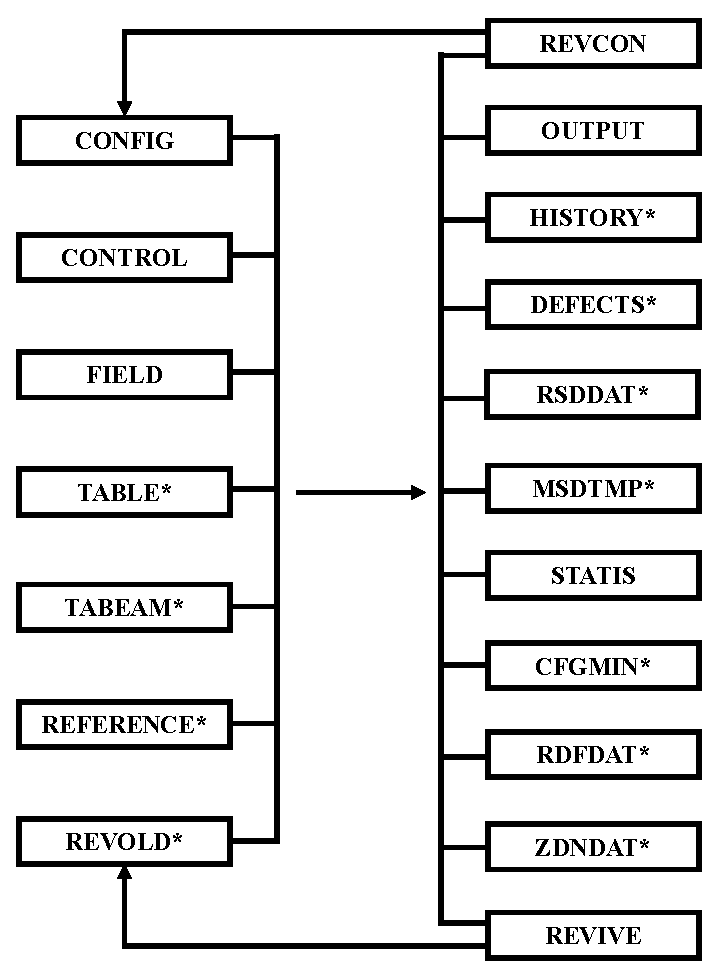
\includegraphics[height=15.0cm]{dlpoly_files.eps}}
\caption[\D input (left) and output (right) files]
{\D input (left) and output (right) files.  {\bf Note}:
files marked with an asterisk are non-mandatory.}
%\vskip 1ex
\end{center}
\end{figure}

\D may require many input files.  However, only CONTROL, CONFIG and
FIELD are mandatory.  The MPOLES and TAB* are complimentary to FIELD
and are only required when opted within.  HISTORY is required when
an old trajectory is opted for re-play in CONTROL. REFERENCE is
optionally required when defect detection is switched on in CONTROL.
REVOLD is required only when the job represents a continuation of a
previous job.  In the following sections we describe the form and
content of these files.

It is worth noting that historically DL\_POLY used hard-coded names
for different I/O files as shown in Figure~\ref{input-files}.
\uline{{\bf This is no longer the case!}}  Upon instructions in
the CONTROL many I/O file name can be overridden with specific,
user-defined filenames (see \hyperref[io]{I/O Control Options}).
Even the CONTROL file can be named differently but in this case the
alternative name {\bf must be passed as a command line argument}
to the \D executable (usually named {\bf DLPOLY.Z}).  Thus the
\D engine can be efficiently embedded and utilised within external
frameworks for user-definable work-flows.

\subsection{The CONTROL File}
\label{control-file}

The CONTROL file is read by the subroutine {\sc read\_control} and
defines the control variables for running a \D job.  (It is also
read by the subroutine {\sc scan\_control} in the {\sc
set\_bounds} routine.)  It makes extensive use of {\bf directives}
and {\bf keywords}.  Directives are character strings that appear
as the first entry on a data record (or line) and which invoke a
particular operation or provide numerical parameters.  Also
associated with each directive may be one or more keywords, which
may qualify a particular directive by, for example, adding extra
options.  Directives can appear in any order in the CONTROL file,
except for the {\bf finish} directive which marks the end of the
file.  Some of the directives are mandatory (for example the {\bf
timestep} directive that defines the timestep), others are
optional.

This way of constructing the file is very convenient, but it has
inherent dangers.  It is, for example, quite easy to specify
contradictory directives, or invoke algorithms\index{algorithm}
that do not work together.  By large \D tries to sort out these
difficulties and print helpful error messages, but it does not
claim to be fully foolproof.  Another common mistake is to specify
more than once a directive that has no contradictory, disabling,
altering or antagonistic directives - then the one specified
last will be used as a control directive (for example
{\bf densvar, equil, steps, press, mxshak, shake, ...}).
Fortunately, in most cases the CONTROL file will be small and
easy to check visually.  It is important to think carefully about
a simulation beforehand and ensure that \D is being asked to do
something that is physically reasonable.  It should also be
remembered that the present capabilities the package may not
allow the simulation required and it may be necessary for you
yourself to add new features.

An example CONTROL file appears below.  The directives and
keywords appearing are described in the following section.  The
example lists all possible and not mutually excluding directives
in a particular order.  Although this order is not mandatory, it
is highly recommended.

\begin{lstlisting}
TITLE RECORD: DL_POLY_4 SAFE ORDER OF CONTROL DIRECTIVES

# I/O REDIRECT
io output  my-dl_poly-run
io config  CONFIG-CDS-generated
io field   FILED-dl_field.out
io history new-trajectory
io revive  REVIVE-2ps-run
io revold  REVIVE-1ps-run
io revcon  REVCON-100k-output

# I/O READ: METHOD, READER COUNT, BATCH & BUFFER SIZES
io read  mpiio        2 2000000 20000

# I/O WRITE: METHOD, TYPE, WRITER COUNT, BATCH & BUFFER SIZES
io write mpiio sorted 8 2000000 20000

# SYSTEM REPLICATION & IMPACT OPTION
nfold              10 10 10
impact 1 2000 7.5 1.0 2.0 3.0

# DENSITY VARIATION ARRAY BOOST
densvar                  10 %

# INDEX AND VERIFICATION BYPASS AND NO TOPOLOGY REPORTING
no index
no strict
no topology

# INTERACTIONS BYPASS
no electostatics
no vdw

# APPLY MIXING TO ALLOWED & AVAILABLE VDW CROSS INTERACTIONS
# Lorentz-Berthelot || Fender-Halsey || Hogervorst (good hope) || Halgren HHG || Tang-Toennies
vdw mixing Lorentz

# DIRECT CALCULATION OF VDW/METAL INTERACTIONS INSTEAD OF
# EVALUATION BY SPLINING OVER TABULATED VALUES IN MEMORY
vdw direct
metal direct

# FORCE-SHIFT VDW INTERACTIONS SO THAT ENERGY AND FORCE
# CONTRIBUTIONS FALL SMOOTHLY TO ZERO WHEN APPROACHING R_CUT
vdw shift

# RANDOM NUMBER GENERATOR SEEDING
seed 100 200 300

# SLAB SIMULATION PARALLEL CONTROL
slab

# RESTART OPTIONS
restart noscale
dump                 1000     steps

# SYSTEM TARGET TEMPERATURE AND PRESSURE
temperature           300.0   Kelvin
pressure                0.001 k-atmospheres

# SYSTEM CUTOFFS AND ELECTROSTATICS
rcut                   10.0  Angstroms
rpad                    0.35 Angstroms
rvdw                    8.0  Angstroms
subcelling threshold   50.0  particles
exclude
epsilon                 1.0
ewald precision         1.0e-5
ewald evaluate          4

# RELAXED SHELL MODEL TOLERANCE
rlxtol                  1.0

# CONSTRANTS ITERATION LENGTH and TOLERANCE
mxshak                250 cycles
shake                   1.0e-5

# INTEGRATION FLAVOUR, ENSEMBLE AND PSEUDO THERMOSTAT
integration velocity verlet
ensemble nst berendsen 0.5 1.5
pseudo langevin   2.0 150.0

# INTEGRATION TIMESTEP
variable timestep       0.001 pico-seconds
mindis                  0.03  Angstroms
maxdis                  0.10  Angstroms
mxstep                  0.005 pico-seconds

# SUMULATION & EQUILIBRATION LENGTH
steps               10000 steps
equilibration        1000 steps

# EQUILIBRATION DIRECTIVES
zero fire
cap                   500 kT/Angstrom
scale                   5 steps
regauss                 3 steps
minimise force      20  1.0    0.00001
optimise energy         0.001  0.00005

# STATISTICS
collect
stack                  50 deep
stats                  10 steps

# OUTPUT
print                  20 steps

# HISTORY
replay
trajectory        20 30 0

# DEFECTS TRAJECTORY - DEFECTS
defects           40 15 0.75

# DISPLACEMENTS TRAJECTORY - RSDDAT
displacements     70 10 0.25

# MSDTMP
msdtmp           1000 100

# INTRAMOLECULAR PDF ANALYSIS BY TYPE IF PRESENT
analyse  bonds       sample every 100  nbins 250  rmax 5.0
analyse  angles      sample every 100  nbins 360  # [ 0 : pi]
analyse  dihedrals   sample every 100  nbins 720  # [-pi: pi]
analyse  inversions  sample every 100  nbins 360  # [ 0 : pi]

# INTRAMOLECULAR PDF ANALYSIS FOR ALL TYPES PRESENT
analyse  all         sample every 100  nbins 1000  rmax 5.0

# PRINT ANY DEFINED INTER-(RDF->VDW) & INTRA-(bonded) MOLECULAR PDF ANALYSIS
print analysis

# RDF & Z-DENSITY
binsize                 0.05 Angstroms
rdf                     7    steps
print rdf
zden                    7    steps
print zden

# EXECUTION TIME
job time             1000 seconds
close time             10 seconds

# FINISH
finish
\end{lstlisting}

\subsubsection{The CONTROL File Format}

The file is free-formatted and not case-sensitive.  Every line is
treated as a command sentence (record).  Commented records
(beginning with a \#) and blank lines are not processed and may be
added to aid legibility (see example above).  Records must be
limited in length to 200 characters.  Records are read in words
({\bf directives} and additional {\bf keywords} and {\bf
numbers}), as a word must not exceed 40 characters in length.
Words are recognised as such by separation by one or more space
characters.  Additional annotation is not recommended but may be
added onto a directive line after the last control word in it.

\begin{itemize}
\item The first record in the CONTROL file is a header (up to 100
characters long) to aid identification of the file.
\item The last record is a {\bf finish} directive, which marks
the end of the input data.
\end{itemize}

Between the header and the {\bf finish} directive, a wide choice
of control directives may be inserted.  These are described below.

\subsubsection{The CONTROL File Directives}
\label{control_options}

\noindent {\bf Note} that in some cases additional keywords, shown in
brackets ``(...)'', may also be supplied in the directives, or
directives may be used in a long form.  However, it is strongly
recommended that the user uses only the {\bf bold} part of these
directives.

The \uline{{\bf MAIN LIST}} of directives available is as follows:

\begin{tabbing}
X\=XXXXXXXXXXXXXXXXXXXX\=XXXXXXXXXXXXXXXXXXXXXXXXXXXXXXXXXXXX\=\kill
\> \uuline{{\bf directive:}}                    \> \phantom{xxxxxxxxxxxxxxxxx} \uuline{{\bf meaning:}} \\
\>                                              \> \\
\> {\bf ana}lyse {\bf all} (sampling) (every) $f$ {\bf nbins} $n$ {\bf rmax} $r$
                                                \> \phantom{xxxxxxxxxxxxxxxxx} calculate and collect all intramolecular PDFs \\
\>                                              \> \phantom{xxxxxxxxxxxxxxxxx} every $f$ timesteps (default $f~=~1$), using a grid \\
\>                                              \> \phantom{xxxxxxxxxxxxxxxxx} with $n$ bins and bonds cutoff of $r$ \AA~(default r~=~2~\AA). \\
\>                                              \> \\
\> {\bf ana}lyse {\bf bon}ds (sampling) (every) $f$ {\bf nbins} $n$ {\bf rmax} $r$
                                                \> \phantom{xxxxxxxxxxxxxxxxx} calculate and collect bonds PDFs \\
\>                                              \> \phantom{xxxxxxxxxxxxxxxxx} every $f$ timesteps (default $f~=~1$), using a grid \\
\>                                              \> \phantom{xxxxxxxxxxxxxxxxx} with $n$ bins in the range $(0:r]$ (default r~=~2~\AA). \\
\>                                              \> \\
\> {\bf ana}lyse {\bf ang}les (sampling) (every) $f$ {\bf nbins} $n$
                                                \> \phantom{xxxxxxxxxxxxxxxxx} calculate and collect angles PDFs \\
\>                                              \> \phantom{xxxxxxxxxxxxxxxxx} every $f$ timesteps (default $f~=~1$), using a grid \\
\>                                              \> \phantom{xxxxxxxxxxxxxxxxx} with $n$ bins in the range $(0:180]$ (degrees). \\
\>                                              \> \\
\> {\bf ana}lyse {\bf dih}edrals (sampling) (every) $f$ {\bf nbins} $n$
                                                \> \phantom{xxxxxxxxxxxxxxxxx} calculate and collect dihedrals PDFs \\
\>                                              \> \phantom{xxxxxxxxxxxxxxxxx} every $f$ timesteps (default $f~=~1$), using a grid \\
\>                                              \> \phantom{xxxxxxxxxxxxxxxxx} with $n$ bins in the range $(-180:180]$ (degrees). \\
\>                                              \> \\
\> {\bf ana}lyse {\bf inv}ersions (sampling) (every) $f$ {\bf nbins} $n$
                                                \> \phantom{xxxxxxxxxxxxxxxxx} calculate and collect inversions PDFs \\
\>                                              \> \phantom{xxxxxxxxxxxxxxxxx} every $f$ timesteps (default $f~=~1$), using a grid \\
\>                                              \> \phantom{xxxxxxxxxxxxxxxxx} with $n$ bins in the range $(0:180]$ (degrees). \\
\>                                              \> \\
\> {\bf binsize} $f$                            \> set the bin size for radial and z-density distribution functions to \\
\>                                              \> $f$ \AA~ (if $10^{-5}$~\AA~$\le~f~\le~r_{\rm cut}/4$ or undefined, $f$ defaults to $0.05$ \AA) \\
\>                                              \> \\
\> {\bf cap} (forces) $f$                       \> cap forces during equilibration period, $f$ is maximum \\
\>                                              \> cap in units of k$_{B}$T/\AA~~(default $f~=~1000$ k$_{B}$T/\AA) \\
\>                                              \> \\
\> {\bf close time} $f$                         \> set job closure time to $f$ seconds \\
\>                                              \> \\
\> {\bf collect}                                \> include equilibration data in overall statistics \\
\>                                              \> \\
\> {\bf coul}omb                                \> calculate electrostatic forces using direct Coulomb sum\index{direct Coulomb sum}\index{potential!electrostatics} \\
\>                                              \> \\
\> {\bf cut}off $f$ ($\equiv$ {\bf rcut} $f$)   \> set required long-ranged interactions\index{potential!electrostatics} cutoff, $r_{\rm cut}$, to $f$ \AA~ \\
\>                                              \> \\
\> {\bf defe}cts $i~j~f$                        \> write defects trajectory file, DEFECTS, with controls: \\
\>                                              \> $i~=$ start timestep for dumping defects configurations \\
\>                                              \> \phantom{xxx} (default $i~=~0$) \\
\>                                              \> $j~=$ timestep interval between configurations (default $j~=~1$) \\
\>                                              \> $f~=$ site-interstitial cutoff (default $f~=~{\rm Min}\left[0.75,r_{\rm cut}/3\right]$~\AA, \\
\>                                              \> ${\rm Min}\left[0.3,r_{\rm cut}/3\right]$~\AA~$\le~f~\le~{\rm Min}\left[3.5,r_{\rm cut}/2\right]$~\AA) \\
\>                                              \> \\
\> {\bf delr} $f$  ($\equiv$ {\bf rpad} $4f$)   \> \C Verlet shell strip cutoff option is iterpreted \\
\>                                              \> by \D as the {\bf pad}ding ($\equiv$ {\bf rpad}) $f/4$ option, so that \\
\>                                              \> $r_{\rm pad}$ gets set to ${\rm Max}(r_{\rm pad},f_{\rm delr}/4)$ \\
\>                                              \> \\
\> {\bf densvar} $f$                            \> allow for local variation of $\approx f$ \% in the system density \\
\>                                              \> of (i) particles and (ii) any present bonded-like entities (very \\
\>                                              \> useful for extremely non-equilibrium simulations, default $f~=~0$) \\
\> {\bf distan}ce                               \> calculate electrostatic forces using Coulomb sum with \\
\>                                              \> distance dependent dielectric\index{distance dependant dielectric} \\
\>                                              \> \\
\> {\bf disp}lacements $i~j~f$                  \> write displacements trajectory file, RSDDAT, with controls: \\
\>                                              \> $i~=$ start timestep for dumping displacements configurations \\
\>                                              \> \phantom{xxx} (default $i~=~0$) \\
\>                                              \> $j~=$ timestep interval between configurations (default $j~=~1$) \\
\>                                              \> $f~=$ displacement qualifying cutoff (default $f~=~0.15~\AA$) \\
\>                                              \> \\
\> {\bf dump} $n$                               \> set restart data dump interval to $n$ steps (default $n~=~1000$) \\
\>                                              \> \\
\> {\bf ensemble nve}                           \> select NVE ensemble\index{ensemble!NVE} (default ensemble) \\
\>                                              \> \\
\> {\bf ensemble nvt evans}                     \> select NVE$_{kin}$ ensemble\index{ensemble!Evans NVT}, type Evans with \\
\>                                              \> Gaussian constraints thermostat\index{thermostat} \\
\>                                              \> \\
\> {\bf ensemble nvt lang}evin $f$              \> select NVT ensemble\index{ensemble!Langevin NVT}, type Langevin with thermostat\index{thermostat} \\
\>                                              \> relaxation speed (friction) constant $f$ in ps$^{-1}$ \\
\>                                              \> \\
\> {\bf ensemble nvt ander}sen $f_{1}~f_{2}$    \> select NVT ensemble\index{ensemble!Langevin NVT}, type Andersen with $f_{1},~f_{2}$ as the \\
\>                                              \> thermostat\index{thermostat} relaxation time in ps and softness ( $0 \le f_{2} \le 1$) \\
\>                                              \> \\
\> {\bf ensemble nvt ber}endesen $f$            \> select NVT ensemble\index{ensemble!Berendsen NVT}, type Berendsen with thermostat\index{thermostat} \\
\>                                              \> relaxation constant $f$ in ps \\
\>                                              \> \\
\> {\bf ensemble nvt hoover} $f$                \> select NVT ensemble\index{ensemble!Nos\'{e}-Hoover NVT}, type Nose-Hoover with thermostat\index{thermostat} \\
\>                                              \> relaxation constant $f$ in ps \\
\>                                              \> \\
\> {\bf ensemble nvt gst} $f_{1}~f_{2}$         \> select NVT ensemble\index{ensemble!Gentle Stochastic NVT}, type Gentle Stochastic with thermostat\index{thermostat} \\
\>                                              \> relaxation constant $f_{1}$ in ps and Langevin friction $f_{1}$ in ps$^{-1}$ \\
\>                                              \> \\
\> {\bf ensemble nvt ttm} $f_{1}~f_{2}~f_{3}$         \> select NVT ensemble\index{ensemble!Inhomogeneous Langevin NVT}, type inhomogeneous Langevin designed \\
\>                                              \> for use as part of the \index{Two-Temperature Model} two-temperature model (TTM), \\ 
\>                                              \> with thermostat\index{thermostat} relaxation constant $f_{1}$ in ps$^{-1}$, \\
\>                                              \> enhancement of relaxation constant $f_{2}$ in ps$^{-1}$ and \\
\>                                              \> cut-off particle velocity for friction enhancement $f_{3}$ in \AA~ps$^{-1}$ \\
\>                                              \> (defaults: $f_{1} = 0.5$, $f_{2} = 0$, $f_{3} = 50$) \\
\>                                              \> \\
\> {\bf ensemble nvt inhomo}geneous $f_{1}~f_{2}~f_{3}$         \> \phantom{xxxxxxxx} select NVT ensemble\index{ensemble!Inhomogeneous Langevin NVT}, type inhomogeneous Langevin: \\
\>                                              \> \phantom{xxxxxxxx}identical to {\bf ensemble nvt ttm} (see above for constants) \\
\>                                              \> \\
\> {\bf ensemble nvt dpd}\textrm{\textit{\textbf{type}}}~~$\gamma$
                                                \> select NVT ensemble\index{ensemble!DPD}, with a DPD thermostat\index{thermostat} of type
                                                \textrm{\textit{\textbf{s1}}} or \textrm{\textit{\textbf{s2}}} \\
\>                                              \> for Shardlow's splitting of first or second order respectively, \\
\>                                              \> with an {\em optional} system global drag coefficient $\gamma$ in Dalton$/$ps \\
\>                                              \> \\
\> {\bf ensemble npt lang}evin $f_{1}~f_{2}$    \> select NPT ensemble\index{ensemble!Langevin NPT}, type Langevin, with $f_{1},~f_{2}$ as the \\
\>                                              \> thermostat\index{thermostat} and barostat\index{barostat} relaxation speed (friction) constants in ps$^{-1}$ \\
\>                                              \> \\
\> {\bf ensemble npt ber}endsen $f_{1}~f_{2}$   \> select NPT ensemble\index{ensemble!Berendsen NPT}, type Berendsen with $f_{1},~f_{2}$ as the \\
\>                                              \> thermostat\index{thermostat} and barostat\index{barostat} relaxation times in ps \\
\>                                              \> \\
\> {\bf ensemble npt hoover} $f_{1}~f_{2}$      \> select NPT ensemble\index{ensemble!Nos\'{e}-Hoover NPT}, type Nose-Hoover, with $f_{1},~f_{2}$ as the \\
\>                                              \> thermostat\index{thermostat} and barostat\index{barostat} relaxation times in ps \\
\>                                              \> \\
\> {\bf ensemble npt mtk} $f_{1}~f_{2}$         \> select NPT ensemble\index{ensemble!Martyna-Tuckerman-Klein NPT}, type Martyna-Tuckerman-Klein with \\
\>                                              \> $f_{1},~f_{2}$ as the thermostat\index{thermostat} and barostat\index{barostat} relaxation times in ps \\
\>                                              \> \\
\> {\bf ensemble nst lang}evin $f_{1}~f_{2}$    \> select N$\mat{\sigma}$T ensemble\index{ensemble!Langevin N$\sigma$T}, type Langevin with $f_{1},~f_{2}$ as the \\
\>                                              \> thermostat\index{thermostat} and barostat\index{barostat} relaxation speed (friction) constants in ps$^{-1}$ \\
\>                                              \> \\
\> {\bf ensemble nst ber}endsen $f_{1}~f_{2}$   \> select N$\mat{\sigma}$T ensemble\index{ensemble!Berendsen N$\sigma$T}, type Berendsen with $f_{1},~f_{2}$ as \\
\>                                              \> the thermostat\index{thermostat} and barostat\index{barostat} relaxation times in ps \\
\>                                              \> \\
\> {\bf ensemble nst hoover} $f_{1}~f_{2}$      \> select N$\mat{\sigma}$T ensemble\index{ensemble!Nos\'{e}-Hoover N$\sigma$T}, type Nose-Hoover with $f_{1},~f_{2}$ as \\
\>                                              \> the thermostat\index{thermostat} and barostat\index{barostat} relaxation times in ps \\
\>                                              \> \\
\> {\bf ensemble nst mtk} $f_{1}~f_{2}$         \> select N$\sigma$T ensemble\index{ensemble!Martyna-Tuckerman-Klein N$\sigma$T}, type Martyna-Tuckerman-Klein with \\
\>                                              \> $f_{1},~f_{2}$ as the thermostat\index{thermostat} and barostat\index{barostat} relaxation times in ps \\
\>                                              \> \\
\> {\bf ensemble nst} $Q~f_{1} f_{2}$ {\bf area} \> select NP$_{n}$AT ensemble, type $Q$ (i.e. {\em lang}, {\em ber}, \\
\>                                              \> {\em hoover} or {\em mtk}), with $f_{1},~f_{2}$ as the thermostat\index{thermostat} \\
\>                                              \> and barostat\index{barostat} relaxation times in ps \\
\>                                              \> \\
\> {\bf ensemble nst} $Q~f_{1} f_{2}$ {\bf tens}ion $\gamma$ \> select NP$_{n}\gamma$T ensemble, type $Q$ (i.e. {\em lang}, {\em ber}, \\
\>                                              \> {\em hoover} or {\em mtk}), with $f_{1},~f_{2}$ as the thermostat\index{thermostat} \\
\>                                              \> and barostat\index{barostat} relaxation times in ps and set required \\
\>                                              \> simulation (target/external) surface tension to $\gamma$ dyn/cm \\
\>                                              \> \\
\> {\bf ensemble nst} $Q~f_{1} f_{2}$ {\bf tens} $\gamma$ {\bf semi}
                                                \> \phantom{xxx} select the same NP$_{n}\gamma$T ensemble as above but with \\
\>                                              \> \phantom{xxx} the "semi-anisotropic constraint" so that the\\
\>                                              \> \phantom{xxx} MD cell changes isotropically in the $(x,y)$ plane \\
\>                                              \> \\
\> {\bf ensemble nst} $Q~f_{1} f_{2}$ {\bf orth}orhombic
                                                \> \phantom{xxx} select the NPT anisotropic ensemble for the orthorhombic\\
\>                                              \> \phantom{xxx} MD cell ("orthorhombic constraint" - equivalent to the \\
\>                                              \> \phantom{xxx} NP$_{n}\gamma$T ensemble when $\gamma=0$: NP$_{n}\gamma=0$T ) \\
\>                                              \> \\
\> {\bf ensemble nst} $Q~f_{1} f_{2}$ {\bf orth semi}
                                                \> \phantom{xxx} select the same NP$_{n}\gamma=0$T ensemble as above but with the \\
\>                                              \> \phantom{xxx} "semi-anisotropic constraint" so that the MD cell changes \\
\>                                              \> \phantom{xxx} isotropically in the $(x,y)$ plane ("semi-orthorhombic \\
\>                                              \> \phantom{xxx} constraint" - equivalent to the NP$_{n}\gamma=0$T semi ensemble) \\
\>                                              \> \\
\> {\bf eps}ilon (constant) $f$                 \> set relative dielectric constant to $f$ (default $f~=~1.0$) \\
\>                                              \> \\
\> {\bf equil}ibration (steps) $n$              \> equilibrate system for the first $n$ timesteps (default $n~=~0$) \\
\>                                              \> \\
\> {\bf ewald evalu}ate (every) $n$             \> evaluate the k-space contributions to the Ewald sum\index{Ewald!SPME}\index{potential!electrostatics} \\
\>                                              \> once every $n$ timesteps ($1~\le~n~\le~10$, activated when $n~\ge~2$, \\
\>                                              \> $n~<~1$ or undefined defaults to $n~=~1$, $n~>~10$ defaults to $n~=~4$) \\
\>                                              \> \\
\> {\bf ewald precision} $f$                    \> calculate electrostatic forces using Ewald sum\index{Ewald!SPME}\index{potential!electrostatics} with \\
\>                                              \> automatic parameter optimisation for precission $f$ \\
\>                                              \> ($10^{-20}~\le~f~\le~0.5$, default $f~=~10^{-20}$) \\
\>                                              \> \\
\> {\bf ewald} (sum) $\alpha~k_{1}~k_{2}~k_{3}$ \> calculate electrostatic forces using Ewald sum\index{Ewald!SPME}\index{potential!electrostatics} with \\
\>                                              \> $\alpha~=~$ Ewald convergence parameter in \AA$^{-1}$ \\
\>                                              \> $k1~=$ is the maximum k-vector index in x-direction \\
\>                                              \> $k2~=$ is the maximum k-vector index in y-direction \\
\>                                              \> $k3~=$ is the maximum k-vector index in z-direction \\
\>                                              \> \\
\> {\bf exclu}de                                \> switch on extended coulombic exclusion affecting intra-molecular \\
\>                                              \> interactions such as: chemical bonds and bond angles; as well as \\
\>                                              \> bond constraints between ions that have shells and cores \\
\>                                              \> \\
\> {\bf finish}                                 \> close the CONTROL file (last data record) \\
\>                                              \> \\
\> {\bf impact} $i~j~~~E~~x~y~z$                \> initiate impact on the particle with index $i$ ($i \ge 1$) at timestep \\
\>                                              \> $j$ ($i \ge 0$) with energy $E$ ($E \ge 0$) in kilo-eV and direction \\
\>                                              \> vector $x~y~z$ from the Cartesian origin (centre) of the MD box \\
\>                                              \> (defaults: $i = 1, j = 0, E = 0, x = 1, y = 1, z = 1$) \\
\>                                              \> \\
\> {\bf integrat}or {\em string}                \> set the type of Verlet integrator, where {\em string} can only be \\
\>                                              \> {\em leapfrog} or {\em velocity}, as the later is the default \\
\>                                              \> \\
\> {\bf job time} $f$                           \> set job time to $f$ seconds \\
\>                                              \> \\
\> {\bf maxdis} $f$                             \> set maximum distance allowed in variable timestep (control) \\
\>                                              \> to $f$ \AA~(default $f~=~0.10$ \AA) \\
\>                                              \> \\
\> {\bf metal direct}                           \> enforce the direct calculation of metal interactions defined \\
\>                                              \> by explicit potential forms, i.e. it will not work for metal \\
\>                                              \> alloy systems using the EAM, EEAM, 2BEAM or 2BEEAM (TABEAM) \\
\>                                              \> \\
\> {\bf metal sqrtrho}                          \> swich the TABEAM default of reading embedding functions, \\
\>                                              \> $F(\rho)$, as interpolated over densities, $\rho$, to as \\
\>                                              \> interpolated over $\sqrt{\rho}$, i.e. $F~=~F(\sqrt{\rho})$\\
\>                                              \> \\
\> {\bf mindis} $f$                             \> set minimum distance allowed in variable timestep (control) \\
\>                                              \> to $f$ \AA~(default $f~=~0.03$ \AA) \\
\>                                              \> \\
\> {\bf minim}ise {\em string} $n$ $f$ $s$      \> minimise the instantaneous system configuration every \\
\>                                              \> $n$ steps during equilibration (with respect to the last \\
\>                                              \> equilibration step) using conjugate gradient method (CGM) \\
\>                                              \> with respect to the criterion, {\em string}, tolerance, $f$, and \\
\>                                              \> and optional CGM stepping, $s$, where this criterion can only be: \\
\>                                              \> {\em force} ($1~\le~f~\le~1000$, default $f~=~50$) or \\
\>                                              \> {\em energy} ($0~<~f~\le~0.01$, default $f~=~0.005$) or \\
\>                                              \> {\em distance} (maximum absolute displacement in \AA, \\
\>                                              \> $10^{-6}~\le~f~\le~0.1$, default $f~=~0.005$); \\
\>                                              \> the optional stepping, $s$, default is $\delta t_{instanteneous}^{2}$; the lowest {\em string} \\
\>                                              \> CGM minimised configuration during equilibration is saved \\
\>                                              \> in a file, CFGMIN which has the same format as CONFIG, \\
\>                                              \> {\bf N.B.} thermostat and barostat memory are not erased \\
\>                                              \> \\
\> {\bf msdtmp} $i~j$                           \> write MSDTMP file, containing particles' individual $\sqrt{MSD}$ \\
\>                                              \> (in \AA) and T$_{mean}$ (in Kelvin), with controls: \\
\>                                              \> $i~=$ start timestep for dumping configurations (default $i~=~0$) \\
\>                                              \> $j~=$ timestep interval between configurations (default $j~=~1$) \\
\>                                              \> \\
\> {\bf mult}iple (timestep) $n$                \> act exactly the same as {\bf ewald evalu}ate (every) $n$ option above \\
\>                                              \> \\
\> {\bf mxquat} $n$                             \> set FIQA iterations limit to $n$ (default $n~=~100$) \\
\>                                              \> \\
\> {\bf mxshak} $n$                             \> set shake/rattle iterations limit to $n$ (default $n~=~250$) \\
\>                                              \> \\
\>                                              \> \\
\> {\bf mxstep} $f$                             \> set maximum timestep value in variable timestep (control) to $f$ \\
\>                                              \> ps (no default $f~=~0.0$ ps but if not opted sets to Huge(1.0)) \\
\>                                              \> \\
\> {\bf nfold} $i~j~k$                          \> option to create matching CONFIG\_i\_j\_k and FIELD\_i\_j\_k \\
\>                                              \> for a volumetrically expanded version of the current system \\
\>                                              \> (CONFIG and FIELD) by replicating CONFIG's contents \\
\>                                              \> ($i$, $j$, $k$) times along the MD cell lattice vectors \\
\>                                              \> while preserving FIELD's topology template intact \\
\>                                              \> \\
\> {\bf no elec}                                \> ignore electrostatics in simulation \\
\>                                              \> \\
\> {\bf no ind}ex                               \> ignore particles' indices as read from the CONFIG file \\
\>                                              \> and set particles' indexing by order of reading, \\
\>                                              \> this option assumes that the FIELD topology description \\
\>                                              \> matches the crystallographic sites from the CONFIG file by \\
\>                                              \> their order of reading rather than by their actual indexing \\
\>                                              \> \\
\> {\bf no str}ict                              \> {\bf (i)} abort strict checks such as; on existence of well defined \\
\>                                              \> system cutoff, on contiguity of particles' indices when \\
\>                                              \> connecting CONFIG (crystallographic listing) to FIELD \\
\>                                              \> (topology), on IO when {\bf io} {\em mpiio/direct sorted} is selected, etc., \\
\>                                              \> {\bf (ii)} abort display of warnings, non-leading to error messages \\
\>                                              \> and of iteration cycles in minimisation/relaxation routines, \\
\>                                              \> {\bf (iii)} assume safe defaults for the general simulation cutoff \\
\>                                              \> and its padding, temperature, pressure and job times \\
\>                                              \> \\
\> {\bf no top}ology                            \> skip detailed topology reporting during read of FIELD in OUTPUT \\
\>                                              \> (no FIELD replication), useful for large bio-chemcal simulations \\
\>                                              \> \\
\> {\bf no vafav}eraging                        \> ignore time-averaging of velocity autocorrelation functions \\
\>                                              \> (VAFs), report all calculated VAF profiles for individual species \\
\>                                              \> to VAFDAT files and final profile (for all species) in OUTPUT \\
\>                                              \> \\
\> {\bf no vdw}                                 \> ignore short range (non-bonded)\index{potential!non-bonded} interactions in simulation \\
\>                                              \> \\
\> {\bf no vom}                                 \> ignore Centre of Mass momentum removal during the simulation \\
\>                                              \> \\
\> {\bf optim}ise {\em string} $f$ $s$          \> minimise the system configuration at start during equilibration \\
\>                                              \> using conjugate gradient method (CGM) with respect to the \\
\>                                              \> criterion, {\em string}, tolerance, $f$ and optional CGM \\
\>                                              \> stepping, $s$, where this criterion can only be: \\
\>                                              \> {\em force} ($1~\le~f~\le~1000$, default $f~=~50$) or \\
\>                                              \> {\em energy} ($0~<~f~\le~0.01$, default $f~=~0.005$) or \\
\>                                              \> {\em distance} (maximum absolute displacement in \AA, \\
\>                                              \> $10^{-6}~\le~f~\le~0.1$, default $f~=~0.005$); \\
\>                                              \> the optional stepping, $s$, default is $(\Delta t_{instanteneous})^{2}$; \\
\>                                              \> the CGM minimised configuration is saved \\
\>                                              \> in a file, CFGMIN which has the same format as CONFIG \\
\>                                              \> \\
\> {\bf pad}ding $f$  ($\equiv$ {\bf rpad} $f$) \> set optional padding to the major cutoff, \\
\>                                              \> $r_{\rm cut}$, to $f$ \AA~ ($f \ge {\rm Min}[0.05,0.5\%.r_{\rm cut}]$, default $f~=~0$) \\
\>                                              \> \\
\> {\bf plumed} {\em string} (on$|$off)         \> global on/off switch for a PLUMED calculation  {\em on} is specified \\
\>                                              \> (default {\em on}), if {\em off} is specified all other plumed directives are ignored \\
\>                                              \> \\
\> {\bf plumed input} $<$$filename$$>$          \> starts a PLUMED calculation, if not switched off, sets PLUMED \\
\>                                              \> input to be read from $<$$filename$$>$ (if unspecified the default is \\
\>                                              \> $<$$filename$$>$~=~PLUMED) \\
\>                                              \> \\
\> {\bf plumed log} $<$$filename$$>$            \> starts a PLUMED calculation, if not switched off, and sets \\
\>                                              \> PLUMED logging to be recorded in $<$$filename$$>$ (default \\
\>                                              \> $<$$filename$$>$~=~OUTPUT.PLUMED) \\
\>                                              \> \\
\> {\bf plumed precision} $int$-$val$           \> starts a PLUMED calculation, if not switched off, and sets \\
\>                                              \> PLUMED calculation precision to $int$-$val$ (default $int$-$val$~=~$wp$ - \\
\>                                              \> the \D working precision) \\
\>                                              \> \\
\> {\bf plumed restart} {\em string} (yes$|$no) \> starts a PLUMED calculation, if not switched off, and hints \\
\>                                              \> PLUMED about restarting (default {\em on}), if {\em off} is specified \\
\>                                              \> PLUMED restart accumulators will reinitialised \\
\>                                              \> \\
\> {\bf polar}isation {\em scheme/type} {\bf thole} $f$ \> set possible polarisation scheme to $type$ with \\
\>                                              \> optional global atomic (Thole) dumping factor \\
\>                                              \> (default $f=1.3$ if none are specified in MPOLES), \\
\>                                              \> only $type=CHARMM$ for Druder core-shell polarisation \\
\>                                              \> is currently available!!! \\
\>                                              \> \\
\> {\bf pres}sure $f$                           \> set required system pressure to $f$ katms \\
\>                                              \> (target pressure for constant pressure\index{units!pressure} ensembles) \\
\>                                              \> \\
\> {\bf print} (every) $n$                      \> print system data every $n$ timesteps \\
\>                                              \> \\
\> {\bf print ana}lysis                         \> print any opted for analysis inter- \& and intra-molecular PDFs \\
\>                                              \> in OUTPUT as well as their corresponding files *DAT, *PMF, *TAB \\
\>                                              \> \\
\> {\bf print rdf}                              \> print radial distribution functions \\
\>                                              \> \\
\> {\bf print vaf}                              \> print velocity autocorrelation functions \\
\>                                              \> \\
\> {\bf print zden}                             \> print Z-density profile \\
\>                                              \> \\
\> {\bf pseudo} {\em string} $f_{1}~f_{2}$      \> attach a pseudo thermal bath with a thermostat of type \\
\>                                              \> {\em string}, where string can only be {\em langevin}, {\em gauss} or {\em direct} \\
\>                                              \> (if none is specified then {\em langevin$\rightarrow$direct} are applied \\
\>                                              \> successively), $f_{1}$ is the thickness of the thermostat \\
\>                                              \> layers, attached on the inside of the MD cell boundaries, \\
\>                                              \> in units of \AA~~(default $f{1}~=~2$ \AA), $f_{2}$ is the \\
\>                                              \> thermostat temperature in Kelvin ($f{2}~\ge~1$), which \\
\>                                              \> when unspecified defaults to the system target temperature \\
\>                                              \> \\
\> {\bf quater}nion (tolerance) $f$             \> set quaternion tolerance to f (default $10^{-8}$) \\
\>                                              \> \\
\> {\bf rdf} (sampling) (every) $f$             \> calculate and collect radial distribution functions \\
\>                                              \> every $f$ timesteps (default $f~=~1$) \\
\>                                              \> \\
\> {\bf reaction} (field)                       \> calculate electrostatic forces using reaction field\index{reaction field} electrostatics\index{potential!electrostatics} \\
\>                                              \> \\
\> {\bf reaction} (field) {\bf damp} $\alpha$   \> calculate electrostatic forces using reaction field\index{reaction field} electrostatics\index{potential!electrostatics} \\
\>                                              \> with Fennell \cite{fennell-06a} damping (Ewald-like convergence) \\
\>                                              \> parameter $\alpha$ in \AA$^{-1}$ \\
\>                                              \> \\
\> {\bf reaction} (field) {\bf precision} $f$   \> calculate electrostatic forces using reaction field\index{reaction field} electrostatics\index{potential!electrostatics} \\
\>                                              \> with Fennell \cite{fennell-06a} damping (Ewald-like convergence) \\
\>                                              \> derived by automatic parameter optimisation for precision $f$ \\
\>                                              \> as for Ewald summation ($10^{-20}~\le~f~\le~0.5$, default $f~=~10^{-20}$) \\
\>                                              \> \\
\> {\bf regaus}s (every) $n$                    \> resample the instantaneous system momenta distribution \\
\>                                              \> every $n$ steps (default $n~=~1$) during equilibration \\
\>                                              \> (with respect to the last equilibration step), {\bf N.B.} \\
\>                                              \> any thermostat and barostat memory is also erased \\
\>                                              \> \\
\> {\bf replay} (history)                       \> abort simulation and replay HISTORY to recalculate structural \\
\>                                              \> properties such as RDFs, z-density profiles, defects and \\
\>                                              \> displacements trajectories (execution halts if no property is specified) \\
\>                                              \> \\
\> {\bf replay} (history) {\bf force}           \> abort simulation and replay the HISTORF file (a HISTORY copy) \\
\>                                              \> with full force evaluation driven by FIELD (different from \\
\>                                              \> the one used for the HISTORF generation) \\
\>                                              \> \\
\> {\bf restart}                                \> restart job from end point of previous run \\
\>                                              \> (i.e. continue current simulation, REVOLD required) \\
\>                                              \> \\
\> {\bf restart noscale}                        \> restart job from previous run without scaling \\
\>                                              \> system temperature (i.e. begin a new simulation from \\
\>                                              \> older run without temperature reset, REVOLD is not used) \\
\>                                              \> \\
\> {\bf restart scale}                          \> restart job from previous run with scaling \\
\>                                              \> system temperature (i.e. begin a new simulation from \\
\>                                              \> older run with temperature reset, REVOLD is not used) \\
\>                                              \> \\
\> {\bf rcut} $f$  ($\equiv$ {\bf cut}off $f$)  \> act exactly the same as the {\bf cut}off $f$ option above \\
\>                                              \> \\
\> {\bf rlxtol} $f$ $s$                         \> set the CGM tolerance (on total force gradient), $f$, for the \\
\>                                              \> relaxed shell model (default $f~=~1$ in D~\AA~~ps$^{-2}$) and \\
\>                                              \> optional CGM stepping, $s$, (default $Max(k_{core-shell})/2$) \\
\>                                              \> \\
\> {\bf rpad} $f$  ($\equiv$ {\bf pad}ding $f$) \> act exactly the same as {\bf pad}ding $f$ option above \\
\>                                              \> \\
\> {\bf rvdw} (cutoff) $f$                      \> set required short-ranged interactions cutoff to $f$ \AA \\
\>                                              \> \\
\> {\bf scale} (temperature) (every) $n$        \> rescale system temperature every $n$ steps (default $n~=~1$) \\
\>                                              \> during equilibration (with respect to the last equilibration \\
\>                                              \> step - atomic velocities are scaled collectively), {\bf N.B.} \\
\>                                              \> any thermostat and barostat memory is also erased \\
\>                                              \> \\
\> {\bf seed} $n_{1}~n_{2}~n_{3}$               \> seed control to the random number generator used in the \\
\>                                              \> generation of gaussian distributions and stochastic processes \\
\>                                              \> \\
\> {\bf shake} (tolerance) $f$                  \> set shake/rattle tolerance to $f$ (default $f~=~10^{-6}$) \\
\>                                              \> \\
\> {\bf shift}                                  \> calculate electrostatic forces using force-shifted Coulomb sum\index{force-shifted Coulomb sum} \\
\>                                              \> \\
\> {\bf shift damp} $\alpha$                    \> calculate electrostatic forces using force-shifted Coulomb sum\index{force-shifted Coulomb sum} \\
\>                                              \> with Fennell \cite{fennell-06a} damping (Ewald-like convergence) \\
\>                                              \> parameter $\alpha$ in \AA$^{-1}$ \\
\>                                              \> \\
\> {\bf shift precision} $f$                    \> calculate electrostatic forces using force-shifted Coulomb sum\index{force-shifted Coulomb sum} \\
\>                                              \> with Fennell \cite{fennell-06a} damping (Ewald-like convergence) \\
\>                                              \> derived by automatic parameter optimisation for precision $f$ \\
\>                                              \> as for Ewald summation ($10^{-20}~\le~f~\le~0.5$, default $f~=~10^{-20}$) \\
\>                                              \> \\
\> {\bf slab}                                   \> limits the number of processors in z-direction to 2 \\
\>                                              \> for slab simulations \\
\>                                              \> \\
\> {\bf spme evalu}ate (every) $n$              \> act exactly the same as {\bf ewald evalu}ate (every) $n$ \\
\>                                              \> \\
\> {\bf spme precision} $f$                     \> act exactly the same as {\bf ewald precision} $f$ \\
\>                                              \> \\
\> {\bf spme} (sum) $\alpha~k_{1}~k_{2}~k_{3}$  \> calculate electrostatic forces using Ewald sum\index{Ewald!SPME}\index{potential!electrostatics} with \\
\>                                              \> $\alpha~=~$ Ewald convergence parameter in \AA$^{-1}$ \\
\>                                              \> $k1~=$ is twice the maximum k-vector index in x-direction \\
\>                                              \> $k2~=$ is twice the maximum k-vector index in y-direction \\
\>                                              \> $k3~=$ is twice the maximum k-vector index in z-direction \\
\>                                              \> \\
\> {\bf stack} (size) $n$                       \> set rolling average stack to {\em n} timesteps \\
\>                                              \> \\
\> {\bf stats} (every) $n$                      \> accumulate statistics data every $n$ timesteps \\
\>                                              \> \\
\> {\bf steps} $n$                              \> run simulation for $n$ timesteps (default $n~=~0$, \\
\>                                              \> corresponding to a "dry" run) \\
\>                                              \> \\
\> {\bf subcell}ing (threshold) (density) $f$   \> set the subcelling threshold density of particles per link cell below \\
\>                                              \> which decreasing link-cell size stops $f$ ($f~\ge~1.0$, default $f~=~50.0)$) \\
\>                                              \> \\
\> {\bf temp}erature $f$                        \> set required simulation temperature to $f$ Kelvin \\
\>                                              \> (target temperature for constant temperature\index{units!temperature} ensembles) \\
\>                                              \> \\
\> {\bf traj}ectory $i~j~k$                     \> write HISTORY file with controls: \\
\>                                              \> $i~=$ start timestep for dumping configurations (default $i~=~0$) \\
\>                                              \> $j~=$ timestep interval between configurations (default $j~=~1$) \\
\>                                              \> $k~=$ data level (default $k~=~0$, see Table~\ref{keytrj}) \\
\>                                              \> \\
\> {\bf ttm amin} $n$                 \> sets minimum number of atoms required in each ionic temperature \\
\>                                              \> cell (CIT) to ensure cell is active (default $n~=~1$) \\
\>                                              \> \\
\> {\bf ttm atomdens} $f$          \> sets atomic density, used to convert specific heat capacities to \\
\>                                              \> volumetric heat capacities, to $f$ (default $f$ set by system \\ 
\>                                              \> configuration) \\
\>                                              \> \\
\> {\bf ttm bcs} $Q$                  \> sets electronic temperature boundary conditions for \index{Two-Temperature Model}two-temperature\\
\>                                              \> model (TTM) to type $Q$, where $Q$ can be: \\
\>                                              \> {\em periodic}: periodic boundaries in all directions \\
\>                                              \> {\em dirich}: Dirichlet boundaries in all directions with simulation \\
\>                                              \> temperature as constant value \\
\>                                              \> {\em neumann}: Neumann (zero-flux) boundaries in all directions\\
\>                                              \> {\em robin} $f$: Robin boundaries in all directions, leaking temperature \\
\>                                              \> fraction $f$ (default $f~=~0.96$) \\
\>                                              \> {\em xydirich}: Dirichlet boundaries in x- and y- directions, \\
\>                                              \> Neumann (zero-flux) boundary in z-direction \\
\>                                              \> {\em xyrobin} $f$: Robin boundaries in x- and y-directions (default $f~=~0.96$),  \\
\>                                              \> Neumann (zero) boundary in z-direction \\
\>                                              \> \\
\> {\bf ttm ceconst} $f$             \> sets constant electronic specific heat capacity to $f$ $k_B$/atom \\
\>                                              \> (default $f~=~1$) \\
\>                                              \> \\
\> {\bf ttm celin} $f_{1}~f_{2}$  \> sets electronic specific heat capacity to linear function of temperature \\
\>                                              \> with maximum value of $f_{1}$ $k_B$/atom at and beyond Fermi temperature \\
\>                                              \> $f_{2}$ K \\
\>                                              \> \\
\> {\bf ttm cetab}                       \> sets electronic volumetric heat capacity (equal to specific heat capacity \\ 
\>                                              \> divided by density) based on tabulated values given in additional file \\
\>                                              \> (Ce.dat) \\
\>                                              \> \\
\> {\bf ttm cetanh} $f_{1}~f_{2}$  \> sets electronic specific heat capacity to hyperbolic tangent form, \\
\>                                              \> $C_{e} (T_{e}) = f_{1} \tanh \left(10^{-4} f_{2} T_{e} \right)$, with constants $f_{1}$ $k_B$/atom and $f_{2}$ K$^{-1}$ \\
\>                                              \> \\
\> {\bf ttm deconst} $f$             \> sets constant thermal diffusivity of non-metal system to $f$ m$^2$/s \\
\>                                              \> \\
\> {\bf ttm dedx} $f$                  \> sets electron stopping power of projectile entering electronic system \\
\>                                              \> to $f$ eV/nm (default $f~=~0$): this energy is deposited into electronic \\
\>                                              \> temperature cells (CETs) after equilibration \\
\>                                              \> \\
\> {\bf ttm delta}                        \> specifies temporal energy deposition to electronic system occurs in  \\
\>                                              \> a single thermal diffusion timestep, i.e. as a Dirac delta-like time \\
\>                                              \> pulse \\
\>                                              \> \\
\> {\bf ttm derecip} $f_{1}~f_{2}$ \> sets thermal diffusivity of non-metal system to reciprocal function of \\
\>                                              \> temperature with value at system temperature of $f$ m$^2$/s, holding \\
\>                                              \> constant beyond Fermi temperature $f_{2}$ K \\
\>                                              \> \\
\> {\bf ttm detab}                       \> sets thermal diffusivity of non-metal system based on tabulated \\ 
\>                                              \> values given in additional file (De.dat) \\
\>                                              \> \\
\> {\bf ttm diff} $f$                     \> identical to {\bf ttm deconst} \\
\>                                              \> \\
\> {\bf ttm dyndens}                  \> dynamically recalculate atom density by only including active \\
\>                                              \> ionic temperature cells (CITs), used to convert specific heat \\
\>                                              \> capacities to volumetric heat capacities after energy deposition \\
\>                                              \> \\
\> {\bf ttm gauss} $f_{1}~f_{2}$  \> specifies temporal energy deposition to electronic system as \\
\>                                              \> Gaussian function of time with standard deviation $f_{1}$ ps, lasting \\
\>                                              \> for $2 f_{2}$ standard deviations (defaults: $f_{1}~=~0.001$, $f_{2} = 5$) \\
\>                                              \> \\
\> {\bf ttm keconst} $f$             \> sets constant electronic thermal conductivity of metal system to \\
\>                                              \> $f$ W~m$^{-1}$~K$^{-1}$ \\
\>                                              \> \\
\> {\bf ttm kedrude} $f$             \> sets electronic thermal conductivity of metal system as Drude model \\
\>                                              \> ($K_{e} (T_{e}) = f \frac{T_{e}}{T_{0}}$), with value at system temperature ($T_{0}$) of \\
\>                                              \> $f$ W~ m$^{-1}$~K$^{-1}$ \\
\>                                              \> \\
\> {\bf ttm keinf}                        \> sets infinitely high electronic thermal conductivity \\
\>                                              \> \\
\> {\bf ttm ketab}                       \> sets thermal conductivity based on tabulated values given in \\
\>                                              \> additional file (Ke.dat), using either local ionic temperature from CIT \\
\>                                              \> or system temperature in CETs outside of atomic system \\
\>                                              \> \\
\> {\bf ttm laser} $f_{1}~f_{2}$   \> specifies initial energy deposition into electronic system occurs \\
\>                                              \> due to laser (homogeneously in space) with absorbed fluence \\
\>                                              \> $f_{1}$ mJ cm$^{-2}$ and penetration depth $f_{2}$ nm \\
\>                                              \> \\
\> {\bf ttm laser} $f_{1}~f_{2}~{\bf zdep} $   \> specifies initial energy deposition into electronic system occurs \\
\>                                              \> due to laser, homogeneously in x- and y-directions, exponential decay in \\ 
\>                                              \> z-direction, with maximum absorbed fluence $f_{1}$ mJ cm$^{-2}$ and \\
\>                                              \> penetration depth $f_{2}$ nm \\
\>                                              \> \\
\> {\bf ttm metal}                       \> specifies parameters for metallic system are required for \\
\>                                              \> \index{Two-Temperature Model}two-temperature model, i.e. thermal conductivity \\
\>                                              \> \\
\> {\bf ttm ncit} $n$                   \> set number of coarse-grained ionic temperature (CIT) cells for \\
\>                                              \> \index{Two-Temperature Model}two-temperature model (TTM) in z-direction (default $n~=~10$): \\
\>                                              \>  numbers in x- and y-directions set according to system size \\
\>                                              \> \\
\> {\bf ttm ncet} $n_{1}~n_{2}~n_{3}$   \> set numbers of coarse-grained electronic temperature (CET) cells for \\
\>                                              \> two-temperature model (TTM): $n_{1}$ for x-direction, $n_{2}$ for y-direction,\\
\>                                              \> $n_{3}$ for z-direction (defaults $n_{1,2,3}~=~20)$ \\
\>                                              \> \\
\> {\bf ttm nexp} $f_{1}~f_{2}$  \> specifies temporal energy deposition to electronic system as \\
\>                                              \> decaying exponential function of time with exponential decay \\
\>                                              \> constant $f_{1}$ ps, lasting for $f_{2}$ time constants (until $f_{1} f_{2}$ ps) \\
\>                                              \> (defaults: $f_{1}~=~0.001$, $f_{2} = 5$) \\
\>                                              \> \\
\> {\bf ttm nonmetal}                 \> specifies parameters for non-metallic system are required for \\
\>                                              \> \index{Two-Temperature Model}two-temperature model), i.e. thermal diffusivity \\
\>                                              \> \\
\> {\bf ttm nothvel}                    \> apply inhomogeneous Langevin thermostat to total particle velocities, \\
\>                                              \> overriding default of using thermal velocities (excluding localised flow) \\
\>                                              \> \\
\> {\bf ttm offset} $f$                 \> offsets initial coupling of electronic and ionic systems via inhomogeneous \\
\>                                              \> Langevin thermostat until after $f$ ps (default $f~=~0$) \\
\>                                              \> \\
\> {\bf ttm oneway}                   \> switches on one-way electron-phonon coupling: only switched on \\
\>                                              \> when electronic tempereature is greater than ionic temperature \\
\>                                              \> \\
\> {\bf ttm pulse} $f$                 \> specifies temporal energy deposition to electronic system as  \\
\>                                              \> square pulse of duration $f$ ps (if $f = 0$, treated as Dirac \\
\>                                              \> delta pulse) \\
\>                                              \> \\
\> {\bf ttm redist}ribute              \> redistribute electronic energy in newly-deactivated temperature \\
\>                                              \> cells to nearest active neighbours \\
\>                                              \> \\
\> {\bf ttm sflat}                         \> specifies initial spatial deposition of energy into electronic system \\
\>                                              \> as flat (homogeneous) profile \\
\>                                              \> \\
\> {\bf ttm sgauss} $f_{1}~f_{2}$ \> specifies initial spatial deposition of energy into electronic system \\
\>                                              \> as Gaussian profile at centre of ionic temperature cells with \\
\>                                              \> standard deviation $f_{1}$ nm, cutting off at $f_{2}$ standard \\
\>                                              \> deviations (defaults: $f_{1} = 1$, $f_{2} = 5$) \\
\>                                              \> \\
\> {\bf ttm sigma} $f_{1}~f_{2}$ \> identical to {\bf ttm sgauss} \\
\>                                              \> \\
\> {\bf ttm stats} $n$                 \> accumulate statistics for two-temperature model every $n$ timesteps \\
\>                                              \> in PEAK\_E and PEAK\_I files \\
\>                                              \> \\
\> {\bf ttm thvelz}                      \> apply inhomogeneous Langevin thermostat to particle thermal velocities \\
\>                                              \> in z-direction only (using total velocities in x- and y-directions) \\
\>                                              \> \\
\> {\bf ttm traj} $n$                   \> accumulate profiles of electronic and ionic temperatures every \\
\>                                              \> $n$ timesteps in LATS\_E and LATS\_I files \\
\>                                              \> \\
\> {\bf ttm varg homo}geneous   \> specifies electron-phonon coupling in thermal diffusion source \\
\>                                              \> term and inhomogeneous Langevin thermostat is set dynamically \\
\>                                              \> using mean electronic temperature (homogeneously) from a tabulated \\
\>                                              \> function of electronic temperature in additional file (g.dat) \\
\>                                              \> \\
\> {\bf ttm varg hetero}geneous    \> specifies electron-phonon coupling in thermal diffusion source \\
\>                                              \> term and inhomogeneous Langevin thermostat is set dynamically \\
\>                                              \> using local electronic temperature (heterogeneously) from a tabulated \\
\>                                              \> function of electronic temperature in additional file (g.dat) \\
\>                                              \> \\

\> {\bf vaf} (sampling) (every) $i$ (bin) (size) $n$ \> \phantom{xxxx} calculate and collect velocity autocorrelation function profiles \\
\>                                                   \> \phantom{xxxx} every $i$ timesteps (default $i~=~50$) with a bin size set to $n$ \\
\>                                                   \> \phantom{xxxx} timesteps (default $n~=~2i$, if $i~/ge~100$, or $n~=~100$ otherwise) \\
\>                                              \> \\
\> {\bf timestep} $f$                           \> set timestep to $f$ ps \\
\>                                              \> \\
\> {\bf variable timestep} $f$                  \> variable timestep, start with timestep of $f$ ps \\
\>                                              \> \\
\> {\bf vdw direct}                             \> enforces the direct calculation of van der Waals interactions \\
\>                                              \> defined by explicit potential forms, i.e. it will not work for \\
\>                                              \> systems using tabulated potentials (TABLE) \\
\>                                              \> \\
\> {\bf vdw mix}  {\em rule}                    \> apply the mixing {\em rule} to all specified analytical, \\
\>                                              \> single-species van der Waals potential interactions \\
\>                                              \> to generate cross-species interactions when: \\
\>                                              \> \phantom{x} (i)~~~the latter has not already been specified; \\
\>                                              \> \phantom{x} (ii)~~single species potentials are available \\
\>                                              \> \phantom{x} ~~~~~~(specified) and of the same type; and \\
\>                                              \> \phantom{x} (iii)~their type is allowed to mix, i.e. of \\
\>                                              \> \phantom{x} ~~~~~~12-6 or LJ or DPD or 14-7 or WCA type. \\
\>                                              \> The available mixing {\bf \em rule}s are as follows: \\
\>                                              \> \phantom{x} {\em lore}ntz for the Lorentz-Berthelot type of mixing \\
\>                                              \> \phantom{x} {\em fend}er for the Fender-Halsey type of mixing \\
\>                                              \> \phantom{x} {\em hoge}rvorst for the Hogervorst (good hope) type of mixing \\
\>                                              \> \phantom{x} {\em halg}ren for the Halgren HHG type of mixing \\
\>                                              \> \phantom{x} {\em tang} for the Tang-Toennies type of mixing \\
\>                                              \> \phantom{x} {\em func}tional for the Functional type of mixing \\
\>                                              \> The mixing formulae can be found in Section~\ref{vdw} \\
\>                                              \> \\
\> {\bf vdw shift}                              \> apply a force-shifting procedure to all van der Waals \\
\>                                              \> potentials (except for the shifted-force n-m and dpd ones) \\
\>                                              \> so that the VDW interactions' energy and force contributions \\
\>                                              \> fall to zero smoothly for distances approaching $r_{\rm cut}$, by solving \\
\>                                              \> $\left(\partial U_{new}(r) / \partial r \right)|_{r = r_{\rm cut}} = 0$ and $U_{new}(r)|_{r=r_{\rm cut}}= 0$ for $a$ and $b$ in \\
\>                                              \> $U_{new}(r) = U(r) + a \cdot r + b$ and the using $U_{new}$ instead $U(r)$ \\
\>                                              \> \\
\> {\bf zden} (sampling) (every) $f$            \> calculate and collect the Z-density profile \\
\>                                              \> every $f$ timesteps (default $f~=~1$) \\
\>                                              \> \\
\> {\bf zero} (fire) (every $n$)                \> perform a dynamic "zero temperature" optimisation MD run \\
\>                                              \> during equilibration; if $fire$ is specified then the system \\
\>                                              \> target temperature is assumed, if not then it is reset to \\
\>                                              \> $10$ Kelvin; if $n$ is specified then every $n$ steps \\
\>                                              \> (default $n~=~1$, with respect to the last equilibration step) \\
\>                                              \> {\bf N.B.} thermostat and barostat memory are not erased
\end{tabbing}

\begin{table}[htbp]
\begin{centering}
\caption{\label{keytrj} Internal Trajectory/Defects File Key}
\vskip 1ex
\begin{tabular}{|r|l|}
\hline
{\tt keytrj} & \multicolumn{1}{c|}{meaning} \\
\hline
0 & coordinates only in file \\
1 & coordinates and velocities in file \\
2 & coordinates, velocities and forces in file \\
\hline
\end{tabular}
\vskip 1ex
\end{centering}
\end{table}

\D also offers a \uline{{\bf SPECIAL OPTIONS LIST}} of directives as follows:

\begin{tabbing}
X\=XXXXXXXXXXXXXXXXXXXX\=XXXXXXXXXXXXXXXXXXXXXXXXXXXXXXXXXXXX\=\kill
\> \uuline{{\bf directive:}}                    \> \phantom{xxxxxxxxxxxxxxxxx} \uuline{{\bf meaning:}} \\
\>                                              \> \\
\> {\bf l\_dis}                                 \> check and report on the minimum separation distance \\
\>                                              \> \\
\> {\bf l\_fast}                                \> abandon global safety checks, which gives more speed \\
\>                                              \> to simulations run at too few link cells per domain \\
\>                                              \> regimes by abandoning global safety checks, however, \\
\>                                              \> in case of parallel failures no controlled manner \\
\>                                              \> termination will happen (OS's feedback dependence!!!) \\
\>                                              \> \\
\> {\bf l\_his}                                 \> generate a one frame HISTORY from CONFIG \\
\>                                              \> and terminate straight after \\
\>                                              \> \\
\> {\bf l\_org} $x~~y~~z~~n$                    \> after reading input recast CONFIG's contents in CFGORG by \\
\>                                              \> translating all coordinates along a vector ($x,y,z$), default \\
\>                                              \> (0,0,0), with a configuration level $n$ (default $n=0$) \& terminate \\
\>                                              \> \\
\> {\bf l\_rin}                                 \> read REVOLD in ASCII (default is binary) \\
\>                                              \> \\
\> {\bf l\_rout}                                \> write REVIVE in ASCII (default is binary) \\
\>                                              \> \\
\> {\bf l\_scl} \phantom{xxx} $n$               \> after reading input cast CONFIG's contents into CFGSCL with \\
\> \phantom{xxxxxxxx} $a_{1}~~a_{2}~~a_{3}$     \> a configuration level $n$ (default $n=0$), rescaling all coordinates \\
\> \phantom{xxxxxxxx} $b_{1}~~b_{2}~~b_{3}$     \> within a new lattice defined by the vectors ($\vek{a},\vek{b},\vek{c}$), \\
\> \phantom{xxxxxxxx} $c_{1}~~c_{2}~~c_{3}$     \> each specified on a new line, \& then terminate the run \\
\>                                              \> \\
\> {\bf l\_scr}                                 \> redirect OUTPUT file's contents to the OS's \\
\>                                              \> default output channel (screen, interactive) \\
\>                                              \> \\
\> {\bf l\_tor}                                 \> abandon the production of REVIVE and REVCON \\
\>                                              \> between all Verlet neighbour list pairs at re/start
\end{tabbing}

\subsubsection{I/O Control Options}
\label{io}

\noindent{\bf Note} that historically DL\_POLY used serial I/O read
and write as well as hard-coded names for different I/O files (see
Figure~\ref{input-files}).  However, {\bf (i)} since version 4.01
\D has defaulted to using parallel read and write via MPI-I/O
(but also supporting a variety of alternative options) and
{\bf (ii)} since version 4.09 the program has also introduced the
functionality for user defined I/O filenames, both available via
the CONTROL {\bf io} directives below.  Even the CONTROL file may
be named differently but in this case the alternative name must be
passed as a command line argument to the \D executable (usually named
{\bf DLPOLY.Z}).  It is worth noting that the latter options have
paved the way for user defined work-flows exploitation of the \D engine.

The \uline{{\bf I/O LIST}} of directives available is as follows:

\begin{tabbing}
X\=XXXXXXXXXXXXXXXXXXXX\=XXXXXXXXXXXXXXXXXXXXXXXXXXXXXXXXXXXX\=\kill
\> \uuline{{\bf directive:}}                    \> \phantom{xxxxxxxxxxxxxxxxx} \uuline{{\bf meaning:}} \\
\>                                              \> \\
\> {\bf io read} {\em method}  $j$ $k$ $l$ $e$  \> set the general I/O read interface to: \\
\>                                              \> {\bf \em method} :: {\em mpiio} for MPI-I/O, {\em direct} for parallel direct access \\
\>                                              \> \phantom{x} FORTRAN I/O or {\em master} for traditional master I/O or {\em netcdf} \\
\>                                              \> \phantom{x} for netCDF I/O provided \D is compiled in a \\
\>                                              \> \phantom{x} netCDF-enabled mode (default {\em mpiio}) \\
\>                                              \> \phantom{xxx} {\bf \em j, reader count} :: $1~\le~j~\le~{\tt job~size}$ \\
\>                                              \> \phantom{xxxx} (default $j~=~2^{Int\left[Log\left\{Min({\tt job~size},2\sqrt{\tt job~size})\right\}/Log(2)\right]}$) \\
\>                                              \> \phantom{xxxx} is the designated number of processes to \\
\>                                              \> \phantom{xxxx} carry out I/O read operations simultaneously \\
\>                                              \> {\bf NOTE that {\em k} is not applicable for the {\em master} method} \\
\>                                              \> \phantom{xxx} {\bf \em k, batch size} :: $1~\le~k~\le~10,000,000$ (default $2,000,000$) \\
\>                                              \> \phantom{xxxx} is the maximum number of particle entities in a batch, i.e. \\
\>                                              \> \phantom{xxxx} multiples of ({\em species},{\em index},$\vek{r}$,$\vek{v}$,$\vek{f}$,{\em etc.}), transmitted between \\
\>                                              \> \phantom{xxxx} I/O groups (= I/O readers) for domain distribution purposes \\
\>                                              \> {\bf \em l, buffer size} :: $100~\le~l~\le~100,000$ (default $20,000$) \\
\>                                              \> \phantom{x} is the maximum number of ASCII line records read in a batch \\
\>                                              \> {\bf NOTE that {\em e} is not applicable for the {\em master} method} \\
\>                                              \> \phantom{xxx} {\bf \em e, parallel error check} :: $Y$es (default $N$) \\
\>                                              \> \\
\> {\bf io writ}e {\em method} $rp$ {\em type} $j$ $k$ $l$ $e$ \> set the general I/O write interface to: \\
\>                                              \> {\bf \em method} :: {\em mpiio} for MPI-I/O, {\em direct} for parallel direct access \\
\>                                              \> \phantom{x} FORTRAN I/O or {\em master} for traditional master I/O or {\em netcdf} \\
\>                                              \> \phantom{x} for netCDF I/O provided \D is compiled in a \\
\>                                              \> \phantom{x} netCDF-enabled mode (default {\em mpiio}) \\
\>                                              \> \phantom{x} {\bf WARRNING: {\em direct} is not a platfotm portable} \\
\>                                              \> \phantom{x} {\bf solution (as it fails on LUSTRE but works on GPFS)} \\
\>                                              \> {\bf NOTE that {\em rp} is only applicable for the {\em netcdf} method} \\
\>                                              \> {\bf \em rp, real precision} :: {\em 32bit} or {\em amber} for 32-bit (float), \\
\>                                              \> \phantom{x} otherwise 64-bit (double) is defaulted if unspecified \\
\>                                              \> {\bf \em type} :: {\em sorted} or {\em unsort}ed (DD scrambled) by global index output \\
\>                                              \> \phantom{x} (default {\em sorted}) \\
\>                                              \> \phantom{xxx} {\bf \em j, writer count} :: $1~\le~j~\le~{\tt job~size}$ \\
\>                                              \> \phantom{xxxx} (default $j~=~2^{Int\left[Log\left\{Min({\tt job~size},8\sqrt{\tt job~size})\right\}/Log(2)\right]}$) \\
\>                                              \> \phantom{xxxx} is the designated number of processes to \\
\>                                              \> \phantom{xxxx} carry out I/O write operations simultaneously \\
\>                                              \> {\bf NOTE that {\em k} is not applicable for the {\em master} method} \\
\>                                              \> \phantom{xxx} {\bf \em k, batch size} :: $1~\le~k~\le~10,000,000$ (default $2,000,000$) \\
\>                                              \> \phantom{xxxx} is the maximum number of particle entities in a batch, i.e. \\
\>                                              \> \phantom{xxxx} multiples of ({\em species},{\em index},$\vek{r}$,$\vek{v}$,$\vek{f}$,{\em etc.}), transmitted between \\
\>                                              \> \phantom{xxxx} I/O groups (= I/O writers) for global sorting purposes \\
\>                                              \> {\bf \em l, buffer size} :: $100~\le~l~\le~100,000$ (default $20,000$) \\
\>                                              \> \phantom{x} is the maximum number of ASCII line records written in a batch \\
\>                                              \> {\bf NOTE that {\em e} is not applicable for the {\em master} method} \\
\>                                              \> \phantom{xxx} {\bf \em e, parallel error check} :: $Y$es (default $N$) \\
\>                                              \> \\
\> {\bf io output}  {\it filename}              \> use {\it filename} instead of OUTPUT \\
\>                                              \> \\
\> {\bf io config}  {\it filename}              \> use {\it filename} instead of CONFIG \\
\>                                              \> \\
\> {\bf io field}   {\it filename}              \> use {\it filename} instead of FIELD \\
\>                                              \> \\
\> {\bf io outstat} {\it filename}              \> use {\it filename} instead of STATIS \\
\>                                              \> \\
\> {\bf io history} {\it filename}              \> use {\it filename} instead of HISTORY \\
\>                                              \> \\
\> {\bf io historf} {\it filename}              \> use {\it filename} instead of HISTORF \\
\>                                              \> \\
\> {\bf io revive}  {\it filename}              \> use {\it filename} instead of REVIVE \\
\>                                              \> \\
\> {\bf io revold}  {\it filename}              \> use {\it filename} instead of REVOLD \\
\>                                              \> \\
\> {\bf io revcon}  {\it filename}              \> use {\it filename} instead of REVCON
\end{tabbing}

\subsubsection{Further Comments on the CONTROL File}

\begin{enumerate}
\item A number of the directives (or their {\bf mutually
exclusive} alternatives) are {\bf mandatory}:
\begin{enumerate}
\item {\bf rcut} ($\equiv$ {\bf cut}): specifying the short range forces cutoff.
{\bf It is compulsory in all circumstances as all \D algorithms are
directly or indirectly dependent on it.}
\item {\bf temp} or {\bf zero}: both may specify the system target temperature.
Though not mutually exclusive aim to specify {\bf temp} and {\bf zero} after
in CONTROL.  {\bf Use only one instance of these in CONTROL!}
If a "dry run" is performed (see below) these can be omitted.
\item {\bf timestep} or {\bf variable timestep}: specifying the
simulation timestep.  {\bf Use only one instance of these in
CONTROL!} If a "dry run" is performed (see below) and a timestep
length is not supplied a default one of $0.001$ ps is provided.
\item {\bf ewald/spme sum/precision} \index{Ewald!summation}
or {\bf coul} or {\bf shift} or {\bf distan} or {\bf reaction}
or {\bf no elec}: specifying the required coulombic forces
option.  Apart from {\bf no elec} the rest of the directives are
mutually exclusive from one another.  {\bf If none is specified
then none is applied!}
\end{enumerate}

\item Some directives are optional.  If not specified \D may give
default values if necessary.  (Some but not all defaults are specified
above in the list of directives.)  However fail-safe \D is, not always will
it assume a default value for certain parameters.  To enable \D to
be even more liberal in the fail-safe features, users are recommended
to use {\bf no strict} option.

\item The {\bf steps} and {\bf equilibration} directives have a
default of zero.  If not used or used with their default values a
"dry run" is performed.  This includes force generation and system
dump (REVCON and REVIVE) and, depending on the rest of the options,
may include; velocity generation, force capping, application of the
CGM minimiser, application of the pseudo thermostat, and dumps of
HISTORY, DEFECTS, RDFDAT, ZDNDAT and MSDTMP.  {\bf Note} that, since
no actual dynamics is to be performed, the {\bf temperature} and
{\bf pressure} directives do not play any role and are therefore
not necessary.

\item If the CGM minimiser, {\bf minim}ise, is specified with zero
frequency, it is only applied at timestep zero if
${\bf equilibration}~\ge~{\bf steps}$ (i.e. optimise structure at
start only!).  This is equvalent to using the {\bf optim}ise
directive.  In this way it can be used as a configuration
optimiser at the beginning of the equilibration period or when
a "dry run" ({\bf steps}~$= 0$) is performed (i.e. equilibrate
without any actual dynamics!).  {\bf Note} that the default CGM search
algorithm stepping uses a step that is proportional to the square of
the instantaneous value of the {\bf timestep} and thus its usage in
may lead to algorithm's instability and failure in the cases when
optimisation is applied before any dynamics occurs in a model
system in an unphysical state (i.e. much away from equilibrium)
and/or with an ill/badly defined forcefield for the state.  Hence,
special care (specifying the optional CGM stepping for example)
should be taken when the option is used, especially as {\bf optimise}
or/and in a "dry run" mode with a timestep value too large for the model system state.

\item The {\bf variable timestep} (or also {\bf timestep variable})
option requires the user to specify an initial guess for a
reasonable timestep for the system (in picoseconds).  The simulation
is unlikely to retain this as the operational timestep however, as
the latter may change in response to the dynamics of the system.  The
option is used in conjunction with the default values of {\bf maxdis}
($0.10$~\AA) and {\bf mindis} ($0.03$~\AA), which can also be
optionally altered if used as directives (note the rule that
{\bf maxdis}~$>~2.5$~{\bf mindis} applies).  Also, an additional
{\bf mxstep} (in ps) control can be applied.  These serve as
control values in the variable timestep algorithm, which calculates
the greatest distance a particle has travelled in any timestep
during the simulation.  If the maximum distance is exceeded, the
timestep variable is halved and the step repeated.  If the greatest
move is less than the minimum allowed, the timestep variable is
doubled and the step repeated provided it does not exceed the
user specified {\bf mxstep}.  If it does then it scales to
{\bf mxstep} and the step is repeated.  In this way the integration
timestep self-adjusts in response to the dynamics of the system.
{\bf Note} that this option is abandoned when used in conjunction with
DPD thermostats ({\bf ensemble nvt dpd}\textrm{\textit{\textbf{type}}}~~$\gamma$),
since it cannot be applied efficiently and furthermore it is not
well defined in a DPD sense either.

\item The {\bf job time} and {\bf close time} directives are
required to ensure a controlled close down procedure when a job
runs out of time.  The time specified by the {\bf job time}
directive indicates the total time allowed for the job.  (This
must obviously be set equal to the time specified to the operating
system when the job is submitted.)  The {\bf close time} directive
represents the time \D will require to write and close all the
data files at the end of processing.  This means the {\em
effective} processing time limit is equal to the job time minus
the close time.  Thus when \D reaches the effective job time limit
it begins the close down procedure with enough time in hand to
ensure the files are correctly written.  In this way you may be
sure the restart files etc. are complete when the job terminates.
{\bf Note} that setting the close time too small will mean the job
will crash before the files have been finished.  If it is set too
large \D will begin closing down too early.  How large the close
time needs to be to ensure safe close down is system dependent and
a matter of experience.  It generally increases with increasing
simulation system size.

\item The starting options for a simulation are governed by the
keyword {\bf restart}.  If this is {\bf not} specified in the
control file, the simulation will start as new.  When specified, it
will continue a previous simulation ({\bf restart}) provided all
needed restart files are in place and not corrupted.  If they are
not in place or are found corrupted, it will start a new simulation
without initial temperature scaling of the previous configuration
({\bf restart noscale}).  Internally these options are handled by
the integer variable {\tt keyres}, which is explained in Table~\ref{keyres}.

\begin{table}[htbp]
\begin{centering}
\caption{\label{keyres} Internal Restart Key}
\vskip 1ex
\begin{tabular}{|r|l|}
\hline
{\tt keyres} & \multicolumn{1}{c|}{meaning} \\
\hline
0 & start new simulation from CONFIG file \\
  & and assign velocities from Gaussian distribution \\
1 & continue current simulation \\
2 & start new simulation from CONFIG file \\
  & and rescale velocities to desired temperature \\
3 & start new simulation from CONFIG file \\
  & and {\bf do not} rescale velocities \\
\hline
\end{tabular}
\vskip 1ex
\end{centering}
\end{table}

\item The various {\bf ensemble} options (i.e.
{\bf nve}\index{ensemble!NVE},
{\bf nvt evans}\index{ensemble!Evans NVT},
{\bf nvt ander}sen\index{ensemble!Andersen NVT},
{\bf nvt lang}evin\index{ensemble!Langevin NVT},
{\bf nvt ber}endsen\index{ensemble!Berendsen NVT},
{\bf nvt hoover}\index{ensemble!Nos\'{e}-Hoover NVT},
{\bf nvt ttm} or {\bf nvt inhomo}geneous\index{ensemble!Inhomogeneous Langevin NVT},
{\bf npt lang}evin\index{ensemble!Langevin NPT},
{\bf npt ber}endsen\index{ensemble!Berendsen NPT},
{\bf npt hoover}\index{ensemble!Nos\'{e}-Hoover NPT},
{\bf npt mtk}\index{ensemble!Martyna-Tuckerman-Klein NPT},
{\bf nst lang}evin\index{ensemble!Langevin N$\sigma$T},
{\bf nst ber}endsen\index{ensemble!Berendsen N$\sigma$T},
{\bf nst hoover}\index{ensemble!Nos\'{e}-Hoover N$\sigma$T},
{\bf nst mtk}\index{ensemble!Martyna-Tuckerman-Klein  N$\sigma$T})
are mutually exclusive, though none is mandatory (the default is
the NVE ensemble\index{ensemble!NVE}).  These options are handled
internally by the integer variable {\tt keyens}.  The meaning of
this variable is explained in Table~\ref{keyens}.  The {\bf nst}
keyword is also used in the N$\sigma$T ensembles extension to
NP$_{n}$AT and NP$_{n}\gamma$T ones.  {\bf Note} that
these semi-isotropic ensembles are only correct for infinite
interfaces placed perpendicularly to the z axis!  This means
that the interface is homogenious (unbroken) and continuous
in the (x,y) plane of the MD cell, which assumes that that two
of the cell vectors have a cross product only in the z
direction.  (For example, if the MD box is defined by
its lattice vectors $(\vek{a},\vek{b},\vek{c})$ then
$\vek{a} \times \vek{b} = \pm (0,0,1)$.)
It is the users' responsibility to ensure this holds for
their model system.

\begin{table}[htbp]
\begin{centering}
\caption{\label{keyens} Internal Ensemble Key}
\vskip 1ex
\begin{tabular}{|r|l|}
\hline
{\tt keyens} & \multicolumn{1}{c|}{meaning} \\
\hline
 0 & Microcanonical ensemble\index{ensemble!microcanonical|see{ensemble,NVE}} (NVE) \index{ensemble!NVE} \\
 1 & Evans NVT\index{ensemble!Evans NVT} ensemble (NVE$_{kin}$) \\
10 & Langevin NVT\index{ensemble!Langevin NVT} ensemble \\
11 & Berendsen NVT ensemble\index{ensemble!Berendsen NVT} \\
12 & Nos\'{e}-Hoover NVT ensemble\index{ensemble!Nos\'{e}-Hoover NVT} \\
15 & inhomogenous Langevin NVT\index{ensemble!Inhomogeneous Langevin NVT} ensemble \\
20 & Langevin NPT\index{ensemble!Langevin NPT} ensemble \\
21 & Berendsen NPT ensemble\index{ensemble!Berendsen NPT} \\
22 & Nos\'{e}-Hoover NPT ensemble\index{ensemble!Nos\'{e}-Hoover NPT} \\
23 & Martyna-Tuckerman-Klein NPT ensemble \index{ensemble!Martyna-Tuckerman-Klein NPT} \\
30 & Langevin N$\mat{\sigma}$T\index{ensemble!Langevin N$\sigma$T} ensemble \\
31 & Berendsen N$\mat{\sigma}$T ensemble\index{ensemble!Berendsen N$\sigma$T} \\
32 & Nos\'{e}-Hoover N$\mat{\sigma}$T ensemble\index{ensemble!Nos\'{e}-Hoover N$\sigma$T} \\
33 & Martyna-Tuckerman-Klein N\mat{\sigma}T ensemble \index{ensemble!Martyna-Tuckerman-Klein N$\sigma$T} \\
\hline
\end{tabular}
\vskip 1ex
\end{centering}
\end{table}

\item The {\bf zero} directive, enables a "zero temperature"
optimisation.  If no optional "fire" keyword is added then the
target temperature of the simulation is reset to $10$ Kelvin.
In either case a crude energy minimiser is used to help the
system relax before each integration of the equations of motion.
The function of the minimiser can be summarised as
\begin{equation}
\vek{v}_{i} \leftarrow \left\{ \begin{array} {l@{\quad:\quad}l}
0 & \vek{v}_{i} \cdot \vek{f}_{i} < 0 \\
\vek{f}_{i} \; \frac{\vek{v}_{i}~\cdot~\vek{f}_{i}}
{\vek{f}_{i}~\cdot~\vek{f}_{i}} & \vek{v}_{i} \cdot
\vek{f}_{i} \ge 0
\end{array} \right.
\end{equation}
for systems with free particles only, where $\vek{v}_{i}$ and
$\vek{f}_{i}$ are the force and velocity of particle $i$.  The
algorithm is extended in the case of RBs by including
\begin{eqnarray}
\vek{V}_{j} \leftarrow \left\{ \begin{array} {l@{\quad:\quad}l}
0 & \vek{V}_{j} \cdot \vek{F}_{j} < 0 \\
\vek{F}_{j} \; \frac{\vek{V}_{j}~\cdot~\vek{F}_{j}}
{\vek{F}_{j}~\cdot~\vek{F}_{j}} & \vek{V}_{j} \cdot
\vek{F}_{j} \ge 0
\end{array} \right. \\ \nonumber
\vek{\omega}_{j} \leftarrow \left\{ \begin{array} {l@{\quad:\quad}l}
0 & \vek{\omega}_{j} \cdot \vek{\tau}_{j} < 0 \\
\vek{\tau}_{j} \; \frac{\vek{\omega}_{j}~\cdot~\vek{\tau}_{j}}
{\vek{\tau}_{j}~\cdot~\vek{\tau}_{j}} & \vek{\omega}_{j} \cdot
\vek{\tau}_{j} \ge 0
\end{array} \right.~~,
\end{eqnarray}
where $\vek{V}_{j}$ and $\vek{F}_{j}$ are the velocity and
force of the RB's centre of mass, and $\vek{\omega}_{j}$ and
$\vek{\tau}_{j}$ are the angular velocity and torque of RB $j$.
Measures are taken to conserve the MD cell momentum and the
thermostat's instantaneous kinetic energy.

This must not be thought of as a true energy minimization
method.  {\bf Note} that this optimisation is only applied
when the simulation runs in equilibration mode.

The algorithm is developed in the \D routine {\sc zero\_k\_optimise}.

\item The {\bf impact} $i$ $j$ $E$ $x$ $y$ $z$ directive will
not be activated if the particle index is beyond the one of
the last particle.  The option will fail in a controlled manner
at application time if the particle is found to be in a frozen
state or the shell of an ion or part of a rigid body.  During
application the center of mass momentum is re-zeroed to prevent
any drifts.  The user must take care to have the impact
initiated after any possible equilibration.  Otherwise, the
system will be thermostatted and the impact energy dissipated
during the equilibration.

\item The {\bf pseudo} option is intended to be used in highly
non-equilibrium simulations when users are primarily interested in
the structural changes in the core of the simulated system as the
the MD cell boundaries of the system are coupled to a thermal bath.

The thermal bath can be used with two types of temperature scaling
algorithms - {\bf(i)} Langevin (stochastic thermostat), {\bf(ii)} Gauss
and {\bf(iii)} Direct (direct thermostat).  If no type is specified then
the Langevin temperature control algorithm is applied first followed the
Direct one.  The user is also required to specify the width of the
pseudo thermostat, $f_{1}$ (in \AA), which must be larger than 2~\AA~
and less than or equal to a quarter of minimum width of the MD cell.
The thermostat is an $f_{1}$ \AA~ thick buffer layer attached on the
inside at the MD cell boundaries.

The temperature of the bath is specified by the user, $T~=~f_{2}$
(in Kelvin), which must be larger than 1 Kelvin.  If none is supplied
by the user, $T$ defaults to the system target temperature.

\begin{itemize}
\item {\bf pseudo langevin}

The stochasticity of the Langevin thermostat emulates an infinite
environment around the MD cell, providing a means for ``natural''
heat exchange between the MD system and the heath bath thus aiding
possible heat build up in the system.  In this way the instantaneous
temperature of the system is driven naturally towards the bath
temperature.  Every particle within the thermostat buffer layer is
coupled to a viscous background and a stochastic heat bath, such
that
\begin{eqnarray}
{d \vek{r}_{i}(t) \over d t} &=& \vek{v}_{i}(t) \nonumber \\
{d \vek{v}_{i}(t) \over d t} &=& {{\vek{f}_{i}(t)+\vek{R}_{i}(t)}
\over m_{i}} - \chi (t) \; \vek{v}_{i}(t)~~,
\end{eqnarray}
where $\chi (t)$ is the friction parameter from the dynamics in the
the MD cell and $R(t)$ is stochastic force with zero mean that
satisfies the fluctuation-dissipation theorem:
\begin{equation}
\left< R^{\alpha}_{i}(t)~R^{\beta}_{j}(t^\prime) \right> =
2~\chi(t)~m_{i}~k_{B}T~\delta_{ij}~\delta_{\alpha
\beta}~\delta(t-t^\prime)~~,
\end{equation}
where superscripts denote Cartesian indices, subscripts particle
indices, $k_{B}$ is the Boltzmann constant, $T$ the bath
temperature and $m_{i}$ the particle's mass.  The algorithm is
implemented in routine {\sc pseudo} and has two stages:
\begin{itemize}
\item Generate random forces on all particles within
the thermostat.  Here, care must be exercised to prevent
introduction of non-zero net force when the random forces are added
to the system force field.
\item Rescale the kinetic energy of the thermostat bath so that
particles within have Gaussian distributed kinetic energy with
respect to the target temperature and determine the (Gaussian
constraint) friction within the thermostat:
\begin{equation}
\chi(t) = Max \left( 0, \frac
{\sum_{i} [\vec{f}_{i}(t) + \vec{R}_{i}(t)] \cdot \vec{v}_{i}(t)}
{\sum_{i} m_{i}~\vec{v}_{i}^{2}(t)} \right)~~.
\end{equation}
Care must be exercised to prevent introduction of non-zero net
momentum.  (Users are reminded to use for target temperature the
temperature at which the original system was equilibrated in order
to avoid simulation instabilities.)
\end{itemize}
The effect of this algorithm is to relax the buffer region of the
system on a local scale and to effectively dissipate the incoming
excess kinetic energy from the rest of the system, thus emulating an
infinite-like environment surrounding the MD cell.  The thermostat
width matters as the more violent the events on the inside of the MD
cell, the bigger width may be needed in order to ensure safe
dissipation of the excess kinetic energy.

\item {\bf pseudo Gauss}

\begin{itemize}
\item Rescale the kinetic energy of the thermostat bath so that
particles within have Gaussian distributed kinetic energy with
respect to the target temperature.
\end{itemize}

\item {\bf pseudo direct}

The Direct thermostat is the simplest possible model allowing for
heat exchange between the MD system and the heath bath.  All (mass,
non-frozen) particles within the bath have their kinetic energy
scaled to $1.5~k_{B}T~$ at the end of each time step during the
simulation.  Care is exercised to prevent introduction of non-zero
net momentum when scaling velocities. (Users are reminded to use for
target temperature the temperature at which the original system was
equilibrated in order to avoid simulation instabilities.) Due to the
``unphysical'' nature of this temperature control the thermostat
width does not matter to the same extent as in the case of the
Langevin thermostat.
\end{itemize}

{\bf Note} that embedding a thermostat in the MD cell walls is bound to
produce {\bf wrong ensemble averages}, and instantaneous pressure
and stress build-ups at the thermostat boundary.  Therefore,
ensembles lose their meaning as such and so does the conserved
quantity for true ensembles.  {\em If the {\bf pseudo} thermostat
option is specified without any type of temperature control in
CONTROL then both types will be applied in the order
Langevin$\rightarrow$Direct at each time step during the
simulation}.

The algorithms are developed in the \D routines {\sc pseudo\_vv} and
{\sc pseudo\_lfv} respectively.

\item The {\bf defe}cts option will trigger reading of REFERENCE
(see Section~\ref{reference-file}), which defines a reference MD
cell with particles' positions defining the crystalline lattice
sites.  If REFERENCE is not found the simulation will either \\
{\bf ( i)} halt if the simulation has been restarted, i.e. is a
continuation of an old one - the {\bf restart} option is used in
CONTROL and the REVOLD (see Section~\ref{revold-file}) file has
been provided. \\
or \\
{\bf (ii)} recover using CONFIG (see Section~\ref{config-file})
if it is a new simulation run, i.e {\bf restart} option is not
used in CONTROL or REVOLD has not been provided.

The actual defect detection is based on comparison of the simulated
MD cell to the reference MD cell based on a user defined
site-interstitial cutoff, $R_{def}$,
\begin{equation}
{\rm Min}\left[0.3,r_{\rm cut}/3\right]~\AA~\le~R_{def}~\le~{\rm Min}\left[1.2,r_{\rm cut}/2\right]~\AA \nonumber
\end{equation}
with a default value of ${\rm Min}\left[0.75,r_{\rm cut}/3\right]$~\AA.
(If the supplied value exceeds the limits the simulation execution
will halt).  If a particle, $p$, is located in the vicinity of a
site, $s$, defined by a sphere with its centre at this site and a
radius, $R_{def}$, then the particle is a {\em first hand} claimee
of $s$, and the site is not vacant.  Otherwise, the site is
presumed vacant and the particle is presumed a general interstitial.
If a site, $s$, is claimed and another particle, $p\prime$, is
located within the sphere around it, then $p\prime$ becomes an
interstitial associated with $s$.  After all particles and all sites
are considered, it is clear which sites are vacancies.  Finally,
for every claimed site, distances between the site and its
{\em first hand} claimee and interstitials are compared and the
particle with the shortest one becomes the {\em real} claimee.  If a
{\em first hand} claimee of $s$ is not the {\em real} claimee it
becomes an interstitial associated with $s$.  At this stage it is
clear which particles are interstitials.  The sum of interstitials
and vacancies gives the total number of defects in the simulated MD
cell.

Frozen particles and particles detected to be shells of
polarisable ions are not considered in the defect detection.

{\bf Note} that the algorithm cannot be applied safely if $R_{def}$ is
larger than half the shortest interatomic distance within the
reference MD cell since a particle may; (i) claim more than one
site, (ii) be an interstitial associated with more than one site, or
both (i) and (ii).  On the other hand, low values of $R_{def}$ are
likely to lead to slight overestimation of defects.

If the simulation and reference MD cell have the same number of
atoms then the total number of interstitials is always equal to the
total number of defects.

\item The {\bf disp}lacements option will trigger dump of atom
displacements based on a qualifying cutoff in a trajectory like
manner.  Displacements of atoms from their original position at
the end of equilibration (the start of statistics), $t~=0~$, is
carried out at each timestep.

\item The tolerance and stepping for relaxed shell model {\bf rlxtol},
is a last resort option to aid shell relaxation of systems with very
energetic and/or rough potential surface.  Users are advised to use
it with caution, should there really need be, as the use of high values
for the tolerance (default of 1) may result in physically incorrect
dynamics and small stepping (default $Max(k_{core-shell})/2$) to
expensive force evaluations.

\item The difference between the directives {\bf ewald} and {\bf spme}
is only in the {\bf ewald/spme sum} directive, in which the
{\bf ewald sum} specifies the indices of the maximum k-vector, whereas
the {\bf spme sum} the dimensions of the 3D charge array
(which are exactly twice the maximum k-vector indices).  {\bf Note}
that in either case, \D will carry out the
SPME\index{Ewald!SPME}\index{potential!electrostatics} coulombic evaluation.

\item The force selection directives
{\bf ewald/spme sum/precision}\index{Ewald!summation},
{\bf reaction}, {\bf coul}, {\bf shift}, {\bf dist}, {\bf no elec}
are handled internally by the integer variable {\tt keyfce}.
See Table~\ref{keyfce} for an explanation of this variable.
{\bf Note} that all these options with the exception of the last,
{\bf no elec}, are mutually exclusive.

\begin{table}[htbp]
\begin{centering}
\caption{\label{keyfce} Electrostatics Key}
\vskip 1ex
\begin{tabular}{|r|l|}
\hline
{\tt keyfce} & \multicolumn{1}{c|}{meaning} \\
\hline
\multicolumn{2}{|c|} {Electrostatics are evaluated as follows:}\\
\hline
0  & Ignore electrostatic\index{potential!electrostatics} interactions \\
2  & SPM Ewald summation\index{Ewald!SPME}\index{potential!electrostatics}\\
4  & Coulomb sum with distance dependent dielectric\index{distance dependant dielectric} \\
6  & Standard truncated Coulomb sum\index{direct Coulomb sum} \\
8  & Force-shifted Coulomb sum\index{force-shifted Coulomb sum} \\
10 & Reaction field electrostatics\index{reaction field} \\
\hline
\end{tabular}
\vskip 1ex
\end{centering}
\end{table}

\item {\bf ewald evaluate} or {\bf multiple} are not mutually
exclusive and it is the first instance of these in CONTROL that
is read and applied in the following simulation.

\item The choice of reaction field electrostatics
(directive {\bf reaction}) relies on the specification of the
relative dielectric constant external to the cavity.  This is
specified by the {\bf eps} directive.

\item The directive {\bf ewald/spme evaluate} is only triggered
when {\bf ewald/spme sum/precision} is present.  It sets an infrequent
evaluation of the k-space contributions to the Ewald summation.
Although this option decreases the simulation cost it also inherently
decreases the accuracy of the dynamics.  {\bf Note} that the usage of
this feature may lead to inacuarte or even wrong and unphysical
dynamics as the less frequent the evaluation, the greater the inacuarcy.

\item \D uses two different potential cutoffs.  These are as
follows:
\begin{enumerate}
\item  $r_{\rm cut}$ - the universal cutoff set by {\bf cutoff}.
It applies to the real space part of the electrostatics calculations
and to the van der Waals\index{potential!van der Waals} potentials if
no other cutoff is applied.
\item $r_{\rm vdw}$ - the user-specified cutoff for the van
der Waals potentials set by {\bf rvdw}.  If not specified its value
defaults to $r_{\rm cut}$.
\end{enumerate}

\item Constraint algorithms in \D, SHAKE/RATTLE (see Section~\ref{shake-rattle}),
use default iteration precision of 10$^{-6}$ and limit of iteration
cycles of 250.  Users may experience that during optimisation of a
new built system containing constraints simulation may fail
prematurely since a constraint algorithm failed to converge.
In such cases directives {\bf mxshak} (to increase) and {\bf shake}
(to decrease) may be used to decrease the strain in the system
and stablise the simulation numerics until equilibration is achieved.

\item \D's DD strategy assumes that the local (per domain/node or
link cell) density of various system entities (i.e. atoms, bonds,
angles, etc.) does not vary much during a simulation and some
limits for these are assumed empirically.  This may not the case in
extremely non-equilibrium simulations, where the assumed limits
are prone to be exceeded or in some specific systems where these
do not hold from the start.  A way to tackle such circumstances and
avoid simulations crash (by controlled termination) is to use the
{\bf densvar} $f$ option.  In the {\sc set\_bounds} subroutine \D
makes assumptions at the beginning of the simulation and corrects
the lengths of bonded-like interaction lists arrays ({\tt mxshl,
mxcons, mxrgd, mxteth, mxbond, mxangl, mxdihd, mxinv}) as well as the
lengths of link-cell ({\tt mxlist}) and domain ({\tt mxatms, mxatdm})
lists arrays when the option is activated with $f > 0$.  Greater
values of $f$ will correspond to allocation bigger global arrays
and larger memory consumption by \D during the simulation.
{\bf Note} that this option may demand more memory than available
on the computer architecture.  In such cases \D will terminate
with an array allocation failure message.

\item As a default, \D does not store statistical data during the
equilibration period.  If the directive {\bf collect} is used,
equilibration data will be incorporated into the overall statistics.

\item The {\bf vaf} directive switches on velocity autocorrelation
function (VAF) calculations for individual atomic species in \D
after equilibration or immediately at start if the directive {\bf collect}
is used.  It controls how often VAF profiles are started what the size
of each profile (in timesteps).  Overlapping profiles are possible and
require more memory to store them (and initial velocities) while they
are being calculated.  By default \D will report time-averaged VAF profiles.
This can be overridden using the {\bf no~vafav}eraging directive, which
will instead report individual `instantaneous' VAF profiles.

\item {\bf io {\em action} [{\em options}]} controls how I/O is performed
by \D.  The options can help the performance of I/O
operations within \D for potentially large files during the run.
The form of the command depends on the value of {\bf action},
which may take the value either {\bf read} or {\bf write}.
In general, this command should only be used for tuning the
I/O subsystem in \D for large runs.  For small to average
sized systems the built-in defaults usually suffice.

\begin{enumerate}
\item {\bf io read {\em method} [{\em options}]}

With action set to {\bf read} the {\bf io} command controls how
the reading of large files is performed.  {\em method} controls
how the disk is accessed.  Possible values are {\em mpiio},
in which case MPI-I/O is used, {\em direct}, which uses
parallel FORTRAN direct access files, and {\em master} which
performs all I/O through a master processor, or {\em netcdf}
for netCDF I/O provided \D is compiled in a netCDF-enabled mode.
{\em mpiio} is the recommended method, and for large systems
{\em master} should be avoided.  Available options depend
on which method is to be used, and all are optional in each
case.  Where numerical values are to be supplied specifying
0 or a negative numbers indicates that \D will resort to
the default value.  The possible options are:

\begin{itemize}
\item {\bf io read mpiio$|$direct$|$netcdf [$j$ [$k$ [$l$ [$e$]]]]}

$j$ specifies the number of processors that shall access
the disk.  $k$ specifies the maximum number of particles
that the reading processors shall deal with at any one time.
Large values give good performance, but may results in an
unacceptable memory overhead.  $l$ specifies the maximum
number of particles that the reading processors shall
read from the disk in one I/O transaction.  Large values
give good performance, but may results in an unacceptable
memory overhead.  $e$ accepts $Y$es only to switch global
error checking performed by the I/O subsystem, the default
is $N$o.

\item {\bf io read master [$l$]}

$l$ specifies the maximum number of particles that the
reading process shall read from the disk in one I/O
transaction.  Large values give good performance, but may
results in an unacceptable memory overhead.
\end{itemize}

\item {\bf io writ}e {\bf{\em method} [{\em rp}] {\em type} [{\em options}]}

With action set to {\bf writ}e the {\bf io} command
controls how the writing of large files is performed.
{\em method} controls how the disk is accessed.  Possible
values are {\em mpiio}, in which case MPI-I/O is used,
{\em direct}, which uses parallel FORTRAN direct access
files, and {\em master} which performs all I/O through
a master processor, or {\em netcdf} for netCDF I/O
provided \D is compiled in a netCDF-enabled mode.
{\em mpiio} is the recommended method, and for
large systems {\em master} should be avoided and also
THE DIRECT OPTION IS NOT STRICTLY PORTABLE, and so may
cause problems on some machines.  {\em rp} is an
optional specification, only applicable to {\em netcdf}
method for opting the binary precision for real numbers.
It only takes {\em 32bit} or {\em amber} for 32-bit
(float) precision, otherwise 64-bit (double) precision
is defaulted.  {\em type} controls the ordering of the
particles on output.  Possible values are {\em sort}ed
and {\em unsort}ed.  {\em sort}ed ensures that the
ordering of the particles the default - sequential,
ascending.  Whereas {\em unsort}ed uses the natural internal
ordering of \D which changes during the simulation.
The recommended and default value is {\em sort}ed.  If none
is specified \D defaultes to the {\em sort}ed type of I/O.
It should be noted that the overhead of the {\em sort}ed
otion compared to the {\em unsort}ed is usually very small.
Available options depend on which method is to be used, and
all are optional in each case.  Where numerical values are
to be supplied specifying 0 or a negative numbers
indicates that \D will resort to the default value.
The possible options are:

\begin{itemize}
\item {\bf io writ}e {\bf mpiio$|$direct$|$netcdf [rp] sort$|$unsort [$j$ [$k$ [$l$ [$e$]]]]}

$j$ specifies the number of processors that shall access
the disk.  $k$ specifies the maximum number of particles
that the writing processors shall deal with at any one time.
Large values give good performance, but may results in an
unacceptable memory overhead.  $l$ specifies the maximum
number of particles that the writing processors shall
write to the disk in one I/O transaction.  Large values
give good performance, but may results in an unacceptable
memory overhead.  $e$ accepts $Y$es only to switch global
error checking performed by the I/O subsystem, the default
is $N$o.

\item {\bf io write master sort$|$unsort [$l$]}

$l$ specifies the maximum number of particles that the
writing process shall write to the disk in one I/O
transaction.  Large values give good performance, but may
results in an unacceptable memory overhead.
\end{itemize}
\end{enumerate}

\item The {\bf no vom} option will trigger a default bypass of
the {\sc getvom} routine which will return zero and thus no COM
removal will happen.  {\bf Note that this will lead to COM momentum
accumulation for many though not all ensembles!}.  Such accumulation
will propagate to the generation of flow in the MD cell and ultimately
suppress the thermal motion of the particles in the system, leading to
the so called "frozen ice cube effect"!  It is worth nothing that this
option must be turned on for the correct application of stochastic
dynamics via the langevin temperature control (NVT Langevin)!  If
the option is not applied then the dynamics will lead to peculiar
thermalisation of different atomic species to mass- and system
size-dependent temperatures.

\item The {\bf replay force} option will attempt to open a renamed
HISTORY as HISTORF and instead following any integration scheme specified
in CONTROL read the positions as integration outcomes and proceed with
the usual MD cycle.  There are a couple of restrictions that may lead to
failures of this feature's application.
\begin{itemize}
\item The CONFIG file at (re)start must be the same as the frame
in HISTORF that CONTROL (REVOLD) attempts to (re)start from.

\item If any two HISTORF consecutive frames are too far apart in
time from each other then domain information reallocation follow-up
may break when the feature is used in parallel.
\end{itemize}

\item The {\bf rpad} ($\equiv$ {\bf pad}) option will add extra distance,
$r_{\rm pad}$, if larger than $f \ge {\rm Min}[0.05,0.5\%.r_{\rm cut}]$~\AA,
to the major cutoff, $r_{\rm cut}$, to construct a larger link-cell width,
$r_{\rm lnk}=r_{\rm cut}+r_{\rm pad}$, which will trigger a construction of
a larger Verlet neighbour list (VNL) while at the same time facilitate its
conditional update, rather at every timestpe.  The VNL conditaional update
is check at the end of each tiemstep and triggered only when the most
travelled particle has moved a distance larger than $r_{\rm pad}/2$.  It is
worth noting that padding is at expense of extra memory but if used wisely
it could improve time to solution from 10\% to 100\% depending on force-field
complexity.  If it is too large or too small (that is why the
$f \ge {\rm Min}[0.05,0.5\%.r_{\rm cut}]$~\AA~limit) it will lead to
performace degradation.  It is recomended that $r_{\rm pad}$ is set up at a
value of $\approx 1 \div 5\%$ of the cutoff, $r_{\rm cut}$, as long as the
major link-cell algorithm uses a link-cell decomposition that not worse than
$4 \otimes 4 \otimes 4$ per domain.  For such setups, in practice, one
may expect average compute speedups \footnote{I.e.~I/O effects are excluded
from comparison with a default simulation and comparisons are carried over
a few hundreds of timesteps.  This is usually accounting for over $90\%$ of
the time to solution.} of the order of $10 \div 30\%$ for force-fields
involving the Ewald summation methodology and $60 \div 100\%$ for force-fields
without electrostatics evaluations involving the Ewald summation methodology.

\item The {\bf subcell} option will set the threshold density of particles
per link cell below which subcelling (decreasing link-cell size) stops.  The
default is 50 although experimenting with values between 10 and 100 may
provide sufficient information about a performance sweetspot.  The comparison
condition is carried out on the average density per sub-link cell of each
domain.  Thus subcelling takes into account only the per domain density
variation.  Obviously, the subcelling threshhold is limited to 1 particle per
cell for the sake of safety and sanity reasons.

\item The {\bf exclu}de option will make sure that for all {\em conventional}
(no distance restraints) intra-molecular interactions (bonds, angles,
digedrals, inversions) as well as for CB and RB units any intra-core-shell
interactions fall within the list of excluded interactions.  This is not
a default behaviour.  The option is also triggered by the {\bf polar}isation
option.

\item The various {\bf ttm} options all have the effect of switching on the 
\index{Two-Temperature Model}two-temperature model (TTM), which assumes 
the use of the \index{ensemble!Inhomogeneous Langevin NVT}inhomogeneous 
Langevin NVT ensemble. It is not possible to specify any other ensemble
for TTM-based systems, so the inhomogeneous Langevin NVT ensemble will
always be used in this case, with default values for the friction terms and cut-off
velocity if these are not specified. No implementation of the inhomogeneous 
Langevin ensemble currently exists for rigid bodies. To model metallic systems, 
the thermal conductivity must be specified either as infinitely large, a constant 
value, a linear function of electronic temperature (based on the Drude model) 
or as a tabulated function of temperature, while non-metallic systems require 
a constant thermal diffusivity. Any energy deposition is applied after equilibration.
An additional restart file, DUMP\_E, consisting of electronic temperatures for 
each electronic temperature cell (CET), is produced along with REVCON and 
REVIVE when TTM is switched on. 

\end{enumerate}

\noindent Users are advised to study the example CONTROL files
appearing in the {\em data} sub-directory to see how different
files are constructed.

\subsection{The CONFIG File}
\label{config-file}

The CONFIG file contains the dimensions of the unit cell, the key
for periodic boundary conditions and the atomic labels,
coordinates, velocities and forces.  This file is read by the
subroutine {\sc read\_config} (optionally by {\sc scan\_config})
in the {\sc set\_bounds} routine.  The first few records of a
typical CONFIG file are shown below:

\begin{lstlisting}
IceI structure 6x6x6 unit cells with proton disorder
         2         3               276
  26.988000000000000   0.000000000000000   0.000000000000000
 -13.494000000000000  23.372293600000000   0.000000000000000
   0.000000000000000   0.000000000000000  44.028000000000000
      OW         1
    -2.505228382        -1.484234330        -7.274585343
    0.5446573999        -1.872177437       -0.7702718106
     3515.939287         13070.74357         4432.030587
      HW         2
    -1.622622646        -1.972916834        -7.340573742
     1.507099154        -1.577400769         4.328786484
     7455.527553        -4806.880540        -1255.814536
      HW         3
    -3.258494716        -2.125627191        -7.491549620
     2.413871957        -4.336956694         2.951142896
    -7896.278327        -8318.045939        -2379.766752
      OW         4
    0.9720599243E-01    -2.503798635        -3.732081894
     1.787340483        -1.021777575        0.5473436377
     9226.455153         9445.662860         5365.202509

etc.
\end{lstlisting}

\subsubsection{The CONFIG File Format}

The file is free-formatted and case sensitive for the atom
species names.  Every line is treated as a command sentence
(record).  However, line records are limited to 72 characters
in length.  Records are read in words, as a word must not
exceed 40 characters in length.  Words are recognised as such
by separation by one or more space characters. The first record
in the CONFIG file is a header (up to 72 characters long) to
aid identification of the file.  Blank and commented lines are not allowed.

\subsubsection{Definitions of Variables in the CONFIG File}

\begin{tabbing}
X\=XXXXXXXX\=XXXXXXXX\=\kill
{\bf record 1} \\
\> {\tt header}  \> a72     \> title line \\
{\bf record 2} \\
\> {\tt levcfg}  \> integer \> CONFIG file key.  See Table~\ref{levcfg} for permitted values \\
\> {\tt imcon}   \> integer \> Periodic boundary key. See Table~\ref{imcon} for permitted values \\
\> {\tt megatm}  \> integer \> Optinal, total number of particles (crystalographic entities) \\
{\bf record 3}   \>         \> omitted if {\tt imcon} = 0 \\
\> {\tt cell(1)} \> real    \> x component of the $a$ cell vector in \AA \\
\> {\tt cell(2)} \> real    \> y component of the $a$ cell vector in \AA \\
\> {\tt cell(3)} \> real    \> z component of the $a$ cell vector in \AA \\
{\bf record 4}   \>         \> omitted if {\tt imcon} = 0 \\
\> {\tt cell(4)} \> real    \> x component of the $b$ cell vector in \AA \\
\> {\tt cell(5)} \> real    \> y component of the $b$ cell vector in \AA \\
\> {\tt cell(6)} \> real    \> z component of the $b$ cell vector in \AA \\
{\bf record 5}   \>         \> omitted if {\tt imcon} = 0 \\
\> {\tt cell(7)} \> real    \> x component of the $c$ cell vector in \AA \\
\> {\tt cell(8)} \> real    \> y component of the $c$ cell vector in \AA \\
\> {\tt cell(9)} \> real    \> z component of the $c$ cell vector in \AA
\end{tabbing}
\noindent {\bf Note} that {\bf record 2} may contain more information
apart from the mandatory as listed above.  If the file has been
produced by \D then it also contains other items intended to help
possible parallel I/O reading. Also, it is worth mentioning that the
periodic boundary conditions (PBC), as specified in Table~\ref{imcon}
and described in detail in Appendix~\ref{boundary-conditions}, refer
generally to a {\bf triclinic type of super-cell}, for which there
are {\bf no symmetry assumptions!  Records 3, 4 and 5} contain the
Cartesian components of the super-cell's lattice vectors in \AA.
\D can only tract triclinic type of super-cells as the only types
of super-cell shapes that are commensurate with the domain decomposition
(DD) parallelisation strategy of it.  However, this is not a restriction
for the replicated data (RD) parallelisation that \C adopts and thus
it can also accept truncated octahedral and rhombic dodecahedral
periodic boundaries.

Subsequent records consists of blocks of between 2 and 4 records
depending on the value of the {\tt levcfg} variable.  Each block
refers to one atom.  The atoms {\bf do not} need to be listed
sequentially in order of increasing index.  Within each block the
data are as follows:
\begin{tabbing}
X\=XXXXXXX\=XXXXXX\=XXXXXX\kill
{\bf record i} \\
\> {\tt atmnam}  \> a8      \> atom name \\
\> {\tt index}   \> integer \> atom index \\
{\bf record ii} \\
\> {\tt xxx}     \> real    \> x coordinate in \AA \\
\> {\tt yyy}     \> real    \> y coordinate in \AA \\
\> {\tt zzz}     \> real    \> z coordinate in \AA \\
{\bf record iii} \>         \> included only if {\tt levcfg} $>0$ \\
\> {\tt vxx}     \> real    \> x component of velocity in \AA/picosecond \\
\> {\tt vyy}     \> real    \> y component of velocity in \AA/picosecond \\
\> {\tt vzz}     \> real    \> x component of velocity in \AA/picosecond \\
{\bf record iv}  \>         \> included only if {\tt levcfg} $>1$ \\
\> {\tt fxx}     \> real    \> x component of force in \AA$\cdot$Dalton/picosecond$^{2}$ \\
\> {\tt fyy}     \> real    \> y component of force in \AA$\cdot$Dalton/picosecond$^{2}$ \\
\> {\tt fzz}     \> real    \> z component of force in \AA$\cdot$Dalton/picosecond$^{2}$
\end{tabbing}
\noindent {\bf Note} that on {\bf record i} only the atom name is
strictly mandatory, any other items are not read by \C but may be
added to aid alternative uses of the file, for example alike DL\_POLY
GUI\index{GUI} \cite{smith-gui}, \C assume that the atoms' indices
are in a sequentially ascending order starting form 1.  However, \D
needs the index or the {\bf no ind}ex option needs to be specified in
the CONTROL file!  It is worth mentioning that \D (as well as \C)
assumes that the origin of Cartesian system with respect to which
the particle positions are specified is the middle of MD cell.  Also,
as both the cell vectors and the particles' positions are specified
in \AA, there is a {\bf fine connection} between them!  This would
not be the case if the particles' positions were kept in reduced space
with fractional coordinates.  Last but not least, it is worth pointing
out that composite entities, such as velocities and forces, have their
units expressed as composites of the default DL\_POLY units as shown in
Section~\ref{units}.

\begin{table}[htbp]
\begin{centering}
\caption{\label{levcfg} CONFIG File Key (record 2)}
\vskip 1ex
\begin{tabular}{|r|l|}
\hline
{\tt levcfg} & \multicolumn{1}{c|}{meaning} \\
\hline
0 & coordinates included in file \\
1 & coordinates and velocities included in file \\
2 & coordinates, velocities and forces included in file \\
\hline
\end{tabular}
\vskip 1ex
\end{centering}
\end{table}

\begin{table}[htbp]
\begin{centering}
\caption{\label{imcon} Periodic Boundary Key (record 2)}
\vskip 1ex
\begin{tabular}{|r|l|}
\hline
{\tt imcon} & \multicolumn{1}{c|}{meaning} \\
\hline
0 & no periodic boundaries \\
1 & cubic boundary conditions\index{boundary conditions!cubic} \\
2 & orthorhombic boundary conditions \\
3 & parallelepiped boundary conditions \\
6 & x-y parallelogram boundary conditions with \\
  & no periodicity in the z direction \\
\hline
\end{tabular}
\vskip 1ex
\end{centering}
\end{table}

\subsubsection{Further Comments on the CONFIG File}

The CONFIG file has the same format as the output file REVCON
(Section~\ref{revcon-file}).  When restarting from a previous run
of \D (i.e. using the {\bf restart}, {\bf restart noscale} or {\bf
restart scale} directives in the CONTROL file - above), the CONFIG
file must be replaced by the REVCON file, which is renamed as the
CONFIG file.  The {\sl copy} macro in the {\em execute}
sub-directory of \D does this for you.

The CONFIG file has the same format as the optional output file
CFGMIN, which is only produced when the {\bf minimise} ({\bf optimise})
option has been used during an equilibration simulation or a "dry run".

\subsection{The FIELD File}
\label{field-file}

The FIELD file contains the force field information defining the
nature of the molecular forces.  This information explicitly
includes the (site) topology of the system which sequence {\bf must}
be matched (implicitly) in the crystallographic description of the
system in the CONFIG file.  The FIELD file is read by the subroutine
{\sc read\_field}. (It is also read by the subroutine {\sc
scan\_field} in the {\sc set\_bounds} routine.) Excerpts from a
force field file are shown below.  The example is the antibiotic
Valinomycin in a cluster of 146 water molecules:
\begin{lstlisting}
Valinomycin Molecule with 146 SPC Waters
UNITS kcal

MOLECULES    2
Valinomycin
NUMMOLS 1
ATOMS 168
    O        16.0000     -0.4160         1
    OS       16.0000     -0.4550         1
    "          "           "        "
    "          "           "        "
    HC        1.0080      0.0580         1
    C        12.0100      0.4770         1
BONDS 78
harm   31   19 674.000     1.44900
harm   33   31 620.000     1.52600
    "    "    "    "         "
    "    "    "    "         "
harm  168   19 980.000     1.33500
harm  168  162 634.000     1.52200
CONSTRAINTS 90
   20   19    1.000017
   22   21    1.000032
    "    "     "
    "    "     "
  166  164    1.000087
  167  164    0.999968
ANGLES 312
harm   43    2   44  200.00      116.40
harm   69    5   70  200.00      116.40
  "    "    "    "     "           "
  "    "    "    "     "           "
harm   18  168  162  160.00      120.40
harm   19  168  162  140.00      116.60
DIHEDRALS 371
harm    1   43    2   44  2.3000      180.00
harm   31   43    2   44  2.3000      180.00
  "    "    "    "    "     "           "
  "    "    "    "    "     "           "
cos   149   17  161   16  10.500      180.00
cos   162   19  168   18  10.500      180.00
FINISH
SPC Water
NUMMOLS 146
ATOMS  3
    OW       16.0000     -0.8200
    HW        1.0080      0.4100
    HW        1.0080      0.4100
CONSTRAINTS  3
    1    2    1.0000
    1    3    1.0000
    2    3    1.63299
FINISH
VDW   45
C       C         lj   0.12000      3.2963
C       CT        lj   0.08485      3.2518
"       "         "     "            "
"       "         "     "            "
"       "         "     "            "
OW      OS        lj   0.15100      3.0451
OS      OS        lj   0.15000      2.9400
CLOSE
\end{lstlisting}

\subsubsection{The FIELD File Format}

The file is free-formatted and not case-sensitive (except for the site names).
Every line is treated as a command sentence (record).  Commented records
(beginning with a \#) and blank lines are not processed and may be
added to aid legibility (see example above).  Records must be
limited in length to 200 characters.  Records are read in words,
as a word must not exceed 40 characters in length.  Words are
recognised as such by separation by one or more space characters.
The contents of the file are variable and are defined by the use
of {\bf directives}.  Additional information is associated with
the directives.

\subsubsection{Definitions of Variables in the FIELD File}

The file divides into three sections: general information, molecular
descriptions, and non-bonded\index{potential!non-bonded} interaction
descriptions, appearing in that order in the file.

\subsubsection*{General information}

The first viable record in the FIELD file is the title.  The
second is the {\bf units} directive.  Both of these are mandatory.
\begin{tabbing}
X\=XXXXXXXXXX\=XXXXX\=\kill
{\bf record 1} \\
\> header      \> a200 \> field file header \\
{\bf record 2}\\
\> {\bf units} \> a40  \> Unit of energy used for input and output
\end{tabbing}
\noindent The energy units on the {\bf units} directive are
described by additional keywords\index{units!energy}:
\begin{description}
\item[a.] {\bf eV}, for electron-Volts
\item[b.] {\bf kcal}/mol, for k-calories per mol
\item[c.] {\bf kJ}/mol, for k-Joules per mol
\item[d.] {\bf K}elvin/Boltzmann, for Kelvin per Boltzmann
\item[e.] {\bf internal}, for DL\_POLY internal units (10 Joules per mol).
\end{description}

\noindent If no units keyword is entered, DL\_POLY internal units
are assumed for both input and output.  The {\bf units} directive
only affects the input and output interfaces, all internal
calculations are handled using DL\_POLY units.  System input and
output energies are read in {\bf units per MD cell}.

{\bf Note} that all energy bearing potential parameters are read
in terms of the specified energy units.  If such a parameter
depends on an angle then the dependence is read in terms of
radians although the following angle in the parameter sequence
is read in terms of degrees.  As to any rule, there is an exception
- the electrostatic bond potential has no energy bearing parameter!

A third optional record can then be supplied before any molecular
description:
\begin{tabbing}
X\=XXXXXXXXXXXXXX\=XXXXXXXXX\=\kill
{\bf record 3} \\
\> {\bf mult}ipolar order $n$ \> a50, integer \> Electrostatics evaluation to order $n$ poles
\end{tabbing}
\noindent This will later trigger the parsing of the MPOLES file
(see Section~\ref{mpoles-file}) which supplies the multipolar
momenta values of the molecular sites specified in FIELD.  Sites
with specified pole orders, $m$, smaller than the one required, $n$,
will have their $m+1$ to $n$ order poles' momenta zeroed.
Similarly, if sites have momenta of poles of higher order than
the one required, $n$, these will not be processed by \D.

{\bf Note}, although algorithms in \D could in principle handle
any high pole order summation, in practice, however, \D will abort
if the order is higher than hexadecapole (order 4)!  For more
information on this functionality refer to Section~\ref{mpoles}.

\subsubsection*{Molecular details}

It is important for the user to understand that there is an
organisational correspondence between the FIELD file and the
CONFIG file described above.  It is required that the order of
specification of molecular types and their atomic constituents in
the FIELD file follows the order of indices in which they appear
in the CONFIG file.  Failure to adhere to this common sequence
will be detected by \D and result in premature termination of the
job. It is therefore essential to work from the CONFIG file when
constructing the FIELD file.  It is not as difficult as it sounds!

The entry of the molecular details begins with the mandatory
directive:

\noindent {\bf molecules {\em n}}

\noindent where {\em n} is an integer specifying the number of
different {\em types} of molecule appearing in the FIELD file.
Once this directive has been encountered, \D enters the {\em
molecular description} environment in which only molecular
description keywords and data are valid.

Immediately following the {\bf molecules} directive, are the records
defining individual molecules:

\begin{enumerate}

\item {\em name-of-molecule} \\
which can be any character string up to 200 characters in length.
({\bf Note}: this is not a directive, just a simple character string.)

\item {\bf nummols {\em n}} \\
where {\em n} is the number of times a molecule of this type
appears in the simulated system.  The molecular data then follow
in subsequent records:

\item {\bf atoms {\em n}} \\
where {\em n} indicates the number of atoms in this type of
molecule.  A number of records follow, each giving details of the
atoms in the molecule i.e. site names, masses and charges.  Each
record carries the entries:
\begin{tabbing}
X\=XXXXXXXXXXXX\=XXXXXXXXXXXX\=\kill
\> {\tt sitnam} \> a8      \> atomic site name \\
\> {\tt weight} \> real    \> atomic site mass (in Daltons) \\
\> {\tt chge}   \> real    \> atomic site charge (in protons) \\
\> {\tt nrept}  \> integer \> repeat counter \\
\> {\tt ifrz}   \> integer \> `frozen' atom (if {\tt ifrz}$~>~0$)
\end{tabbing}
The integer {\tt nrept} need not be specified if the atom/site is
not frozen (in which case a value of 1 is assumed.)  A number
greater than 1 specified here indicates that the next ({\tt nrept}-1)
entries in the CONFIG file are ascribed the atomic
characteristics given in the current record.  The sum of the
repeat numbers for all atoms in a molecule should equal the number
specified by the {\bf atoms} directive.

\item{\bf shell {\em n}} \\
where {\em n} is the number of core-shell units.  Each of the
subsequent {\em n} records contains:
\begin{tabbing}
X\=XXXXXXXXXXXX\=XXXXXXXXXXXX\=\kill
\> index 1 ($i$) \> integer \> site index of core \\
\> index 2 ($j$) \> integer \> site index of shell \\
\> $k_{2}$       \> real    \> force constant of core-shell spring \\
\> $k_{4}$       \> real    \> quartic (anharmonic) force constant of spring
\end{tabbing}
The spring potential is
\begin{equation}
U(r)=\frac{1}{2}k_{2} r_{ij}^{2}+\frac{1}{4!}k_{4} r_{ij}^{4}~~,
\end{equation}
with the force constant $k_{2}$ entered in units of {\tt engunit}$\times$\AA$^{-2}$
and $k_{4}$ in {\tt engunit}~\AA$^{-4}$, where usually $k_{2} >> k_{4}$.
The {\tt engunit} is the energy unit specified in the {\bf units} directive.

{\bf Note} that the atomic site indices referred to above are
indices arising from numbering each atom in the molecule from 1 to
the number specified in the {\bf atoms} directive for this
molecule.  This same numbering scheme should be used for all
descriptions of this molecule, including the {\bf constraints},
{\bf pmf}, {\bf rigid}, {\bf teth}, {\bf bonds}, {\bf angles},
{\bf dihedrals} and {\bf inversions} entries described below.
\D will itself construct the global indices for all atoms in the systems.

{\bf Note} that \D determines which shell model to use by scanning
shells' weights provided the FIELD file (see Section~\ref{shell-models}).
If all shells have zero weight the \D will choose the relaxed shell
model.  If no shell has zero weight then \D will choose the dynamical
one.  In case when some shells are massless and some are not \D will
terminate execution controllably and provide information about the
error and possible possible choices of action in the OUTPUT file
(see Section~\ref{output-file}).  Shell models' extensions are dealt
according to the user specifications in the FIELD files.

This directive (and associated data records) need not be specified if
the molecule contains no core-shell units.

\item {\bf constraints {\em n}} \\
where {\em n} is the number of constraint bonds in the molecule.
Each of the following {\em n} records contains:
\begin{tabbing}
X\=XXXXXXXXXXXX\=XXXXXXXXXXXX\=\kill
\> index 1    \> integer \> first atomic site index \\
\> index 2    \> integer \> second atomic site index \\
\> bondlength \> real    \> constraint bond\index{constraints!bond} length
\end{tabbing}
This directive (and associated data records) need not be specified
if the molecule contains no constraint
bonds\index{constraints!bond}.  See the note on the atomic indices
appearing under the {\bf shell} directive above.

\item {\bf pmf {\em b}} \\
where {\em b} is the potential of mean force bondlength (\AA).
There follows the definitions of two PMF units:
\begin{enumerate}
\item {\bf pmf unit {\em n1}} \\
where {\em n1} is the number of sites in the first unit.  The subsequent
{\em n1} records provide the site indices and weighting.  Each record contains:
\begin{tabbing}
X\=XXXXXXXXXXXX\=XXXXXXXXXXXX\=\kill
\> index      \> integer \> atomic site index \\
\> weight     \> real    \> site weighting
\end{tabbing}
\item {\bf pmf unit {\em n2}} \\
where {\em n2} is the number of sites in the second unit.  The subsequent
{\em n2} records provide the site indices and weighting.  Each record contains:
\begin{tabbing}
X\=XXXXXXXXXXXX\=XXXXXXXXXXXX\=\kill
\> index      \> integer \> atomic site index \\
\> weight     \> real    \> site weighting
\end{tabbing}
\end{enumerate}
This directive (and associated data records) need not be specified
if no PMF constraints are present\index{constraints!PMF}.  See the
note on the atomic indices appearing under the {\bf shell} directive.

{\bf Note} that if a site weighting is not supplied \D will assume
it is zero.  However, \D detects that all sites in a PMF unit have
zero weighting then the PMF unit sites will be assigned the masses
of the original atomic sites.

The PMF bondlength applies to the distance between the centres of the
two PMF units.  The centre, $\vec{R}_{i}$, of each unit is given by
\begin{equation}
\vek{R}_{i}~=~\frac{\sum_{j=1}^{n_{i}} w_{j}~\vec{r}_{j}}{\sum_{j=1}^{n_{j}} w_{j}}~~,
\end{equation}
where $r_{j}$ is a site position and $w_{j}$ the site weighting.

{\bf Note} that the PMF constraint is intramolecular.  To define
a constraint between two molecules, the molecules must be described as
part of the same \D ``molecule''.  \D allows only one type of PMF
constraint per system.  The value of nummols for this molecule
determines the number of PMF constraint in the system.

{\bf Note} that in \D PMF constraints are handeled in every available
ensemble.

\item{\bf rigid {\em n}}\\
where {\em n} is the number of basic rigid units in the molecule.  It is
followed by at least {\em n} records, each specifying the sites in a rigid
unit:
\begin{tabbing}
X\=XXXXXXXXXXXX\=XXXXXXXXXXXX\=\kill
\> m      \> integer \> number of sites in rigid unit \\
\> site 1 \> integer \> first site atomic index \\
\> site 2 \> integer \> second site atomic index \\
\> site 3 \> integer \> third site atomic index \\
\> .. \> .. \> {\em etc.} \\
\> site m \> integer \> m'th site atomic index
\end{tabbing}
Up to 15 sites can be specified on the first record.  Additional records
can be used if necessary.  Up to 16 sites are specified per record thereafter.

This directive (and associated data records) need not be specified if the
molecule contains no rigid units.  See the note on the atomic indices
appearing under the {\bf shell} directive above.

\item{\bf teth {\em n}} \\
where {\em n} is the number of tethered atoms in the molecule.  It
is followed {\em n} records specifying the tehered sites in the
molecule:
\begin{tabbing}
X\=XXXXXXXXXXXX\=XXXXXXXXXXXX\=\kill
\> tether key    \> a4      \> potential key, see Table~\ref{tether-table} \\
\> index 1 ($i$) \> integer \> atomic site index \\
\> variable 1    \> real    \> potential parameter, see Table~\ref{tether-table} \\
\> variable 2    \> real    \> potential parameter, see Table~\ref{tether-table}
\end{tabbing}
The meaning of these variables is given in Table
\ref{tether-table}.

This directive (and associated data records) need not be specified
if the molecule contains no flexible chemical bonds.  See the note
on the atomic indices appearing under the {\bf shell} directive
above.

\begin{table}[htbp]
\begin{centering}
\caption{\label{tether-table} Tethering Potentials}
\vskip 1ex
\begin{tabular}{|l|l|c|c|c|c|}
\hline
key & potential type & \multicolumn{3}{c|}{Variables (1-3)} & functional form \\
\hline
            &            &         &         &         & \\
{\bf harm}  & Harmonic   & $k$     &         &         &
$ U(r) = \frac{1}{2}~k~(r_{i}-r_{i}^{t=0})^{2}$ \\

            &            &         &         &         & \\
{\bf rhrm}  & Restraint  & $k$     & $r_{c}$ &         &
$U(r) = \frac{1}{2}~k~(r_{i}-r_{i}^{t=0})^{2}~~~~~~~~~~~~~~~~~~~:~|r_{i}-r_{i}^{t=0}| \le r_{c}$ \\
            &            &         &         &         &
$U(r) = \frac{1}{2}~k~r_{c}^{2}+k~r_{c}(|r_{i}-r_{i}^{t=0}|-r_{c})~:~|r_{i}-r_{i}^{t=0}|>r_{c}$ \\
            &            &         &         &         & \\
{\bf quar}  & Quartic    & $k$     & $k'$    & $k''$   &
$U(r) = \frac{k}{2}~(r_{i}-r_{i}^{t=0})^{2}+\frac{k'}{3}~(r_{i}-r_{i}^{t=0})^{3}$ \\
            &            &         &         &         &
$+\frac{k''}{4}~(r_{i}-r_{i}^{t=0})^{4}$ \\
            &            &         &         &         & \\
\hline
\end{tabular}
\vskip 1ex
\end{centering}
\end{table}

\item{\bf bonds {\em n}} \\
where {\em n} is the number of flexible chemical bonds in the
molecule.  Each of the subsequent {\em n} records contains:
\begin{tabbing}
X\=XXXXXXXXXXXX\=XXXXXXXXXXXX\=\kill
\> bond key      \> a4      \> potential key, see Table~\ref{bond-table} \\
\> index 1 ($i$) \> integer \> first atomic site index in bond \\
\> index 2 ($j$) \> integer \> second atomic site index in bond \\
\> variable 1    \> real    \> potential parameter, see Table~\ref{bond-table} \\
\> variable 2    \> real    \> potential parameter, see Table~\ref{bond-table} \\
\> variable 3    \> real    \> potential parameter, see Table~\ref{bond-table} \\
\> variable 4    \> real    \> potential parameter, see Table~\ref{bond-table}
\end{tabbing}
The meaning of these variables is given in Table~\ref{bond-table}.

This directive (and associated data records) need not be specified
if the molecule contains no flexible chemical bonds.  See the note
on the atomic indices appearing under the {\bf shell} directive
above.

\begin{table}[htbp]
\begin{centering}
\caption{\label{bond-table} Chemical Bond Potentials}
\vskip 1ex
\begin{tabular}{|l|l|c|c|c|c|c|}
\hline
key & potential type & \multicolumn{4}{c|}{Variables (1-4)} & functional form \\
\hline
            &                    &            &          &          &       & \\
{\bf tab}   & Tabulation, see     &            &          &          &       & tabulated potential \\
{\bf -tab}  & Sections~\ref{bond-potentials}~\ref{intra-tables}
                                 &            &          &          &       & in TABBND file \\
            &                    &            &          &          &       & \\
{\bf harm}  & Harmonic           & $k$        & $r_{0}$  &          &       &
$U(r) = \frac{1}{2}~k~(r_{ij}-r_{0})^{2}$ \\
{\bf -hrm}  &                    &            &          &          &       & \\
            &                    &            &          &          &       & \\
{\bf mors}  & Morse              & $E_{0}$    & $r_{0}$  & $k$      &       &
$U(r) = E_{0}~[\{1-\exp(-k~(r_{ij}-r_{0}))\}^{2}-1]$ \\
{\bf -mrs}  &                    &            &          &          &       & \\
            &                    &            &          &          &       & \\
{\bf 12-6}  & 12-6               & $A$        & $B$      &          &       &
$U(r) = \left (\frac{A}{r_{ij}^{12}}\right)-\left(\frac{B}{r_{ij}^{6}}\right)$ \\
{\bf -126}  &                    &            &          &          &       & \\
            &                    &            &          &          &       & \\
{\bf lj}    & Lennard-Jones      & $\epsilon$ & $\sigma$ &          &       &
$U(r) = 4 \epsilon \left[ \left( \frac{\sigma}{r_{ij}} \right)^{12} - \left( \frac{\sigma}{r_{ij}}\right)^{6} \right]$ \\
{\bf -lj}   &                    &            &          &          &       & \\
            &                    &            &          &          &       & \\
{\bf rhrm}  & Restraint          & $k$        & $r_{0}$  & $r_{c}$  &       &
$U(r) = \frac{1}{2}~k~(r_{ij}-r_{0})^{2}~~~~~~~~~~~~~~~~~~~:~|r_{ij}-r_{0}| \le r_{c}$ \\
{\bf -rhm}  &                    &            &          &          &       &
$U(r) = \frac{1}{2}~k~r_{c}^{2}+k~r_{c}(|r_{ij}-r_{0}|-r_{c})~:~|r_{ij}-r_{0}|>r_{c}$ \\
            &                    &            &          &          &       & \\
{\bf quar}  & Quartic            & $k$        & $r_{0}$  & $k'$     & $k''$ &
$U(r) = \frac{k}{2}~(r_{ij}-r_{0})^{2}+\frac{k'}{3}~(r_{ij}-r_{0})^{3}$ \\
{\bf -qur}  &                    &            &          &          &       &
$+\frac{k''}{4}~(r_{ij}-r_{0})^{4}$ \\
            &                    &            &          &          &       & \\
{\bf buck}  & Buckingham         & $A$        & $\rho$   & $C$      &       &
$U(r) = A~\exp\left(-\frac{r_{ij}}{\rho}\right)-\frac{C}{r_{ij}^{6}}$ \\
{\bf -bck}  &                    &            &          &          &       & \\
            &                    &            &          &          &       & \\
{\bf coul}  & Coulomb            & $k$        &          &          &       &
$U(r) = k \cdot U^{Electrostatics}(r_{ij}) \; \left(= \frac{k}{4\pi\epsilon_{0}\epsilon}\frac{q_{i}q_{j}}{r_{ij}}\right)$ \\
{\bf -cul}  &                    &            &          &          &       & \\
            &                    &            &          &          &       & \\
{\bf fene}  & Shifted$^{*}$ FENE & $k$        & $R_{o}$  & $\Delta$ &       &
$U(r) = -0.5~k~R_{o}~ln\left[1-\left(\frac{r_{ij}-\Delta}{R_{o}^{2}}\right)^{2}\right]~:~r_{ij} < R_{o} + \Delta$ \\
{\bf -fne}  & \cite{warner-72a,bird-77a,grest-86a} & &   &          &       &
$U(r) = \infty~~~~~~~~~~~~~~~~~~~~~~~~~~~~~~~~~~~~:~r_{ij} \ge R_{o} + \Delta$ \\
            &                    &            &          &          &       & \\
{\bf mmst}  & MM3 bond stretch   & $k$        & $r_{o}$  &          &       &
$U(r) = k~\delta^{2}\left[1-2.55~\delta+(7/12)~2.55^{2}~\delta^{2}\right]~;~\delta~ = r-r_{o}$ \\
{\bf -mst}  & \cite{allinger-89a} &           &          &          &       & \\
            &                    &            &          &          &       & \\
\hline
\end{tabular}
\vskip 1ex
\end{centering}
$^{*}$ Note: $\Delta$ defaults to zero if $|\Delta| > 0.5~R_{o}$ or
if it is not specified in the FIELD file.

{\bf Note:} Bond potentials\index{potential!bond} with a dash (-) as
the first character of the keyword, do not contribute to the {\em
excluded atoms list} (see Section~\ref{force-field}).  In this case
\D will also calculate the non-bonded\index{potential!non-bonded}
pair potentials between the described atoms, unless these are
deactivated by another potential specification.
\vskip 1ex
\end{table}

\item{\bf angles {\em n}} \\
where {\em n} is the number of valence
angle\index{potential!valence angle} bonds in the molecule.  Each
of the {\em n} records following contains:
\begin{tabbing}
X\=XXXXXXXXXXXX\=XXXXXXXXXXXX\=\kill
\> angle key     \> a4      \> potential key, see Table~\ref{angle-table} \\
\> index 1 ($i$) \> integer \> first atomic site index \\
\> index 2 ($j$) \> integer \> second atomic site index (central site) \\
\> index 3 ($k$) \> integer \> third atomic site index \\
\> variable 1    \> real    \> potential parameter, see Table~\ref{angle-table} \\
\> variable 2    \> real    \> potential parameter, see Table~\ref{angle-table} \\
\> variable 3    \> real    \> potential parameter, see Table~\ref{angle-table} \\
\> variable 4    \> real    \> potential parameter, see Table~\ref{angle-table}
\end{tabbing}
The meaning of these variables is given in Table
\ref{angle-table}.

This directive (and associated data records) need not be specified
if the molecule contains no angular terms.  See the note on the
atomic indices appearing under the {\bf shell} directive above.

\begin{table}[htbp]
\begin{centering}
\caption{\label{angle-table} Valence Angle Potentials}
\vskip 1ex
\begin{tabular}{|l|l|c|c|c|c|c|}
\hline
key & potential type & \multicolumn{4}{c|}{Variables (1-4)} & functional form\dag \\
\hline
           &                     &     &              &            &            & \\
{\bf tab}  & Tabulation, see      &     &              &            &            & tabulated potential \\
{\bf -tab} & Sections~\ref{angle-potentials}~\ref{intra-tables}
                                 &     &              &            &            & in TABANG file \\
           &                     &     &              &            &            & \\
{\bf harm} & Harmonic            & $k$ & $\theta_{0}$ &            &            &
$U(\theta) = {k \over 2}~(\theta - \theta_{0})^{2}$ \\
{\bf -hrm} &                     &     &              &            &            & \\
           &                     &     &              &            &            & \\
{\bf quar} & Quartic             & $k$ & $\theta_{0}$ & $k'$       & $k''$      &
$U(\theta) = {k \over 2}~(\theta - \theta_{0})^{2} + {k'\over 3}(\theta - \theta_{0})^{3} + {k''\over 4}(\theta - \theta_{0})^{4}$ \\
{\bf -qur} &                     &     &              &            &            & \\
           &                     &     &              &            &            & \\
{\bf thrm} & Truncated harmonic  & $k$ & $\theta_{0}$ & $\rho$     &            &
$U(\theta) = {k \over 2}~(\theta - \theta_{0})^{2} \exp[-(r_{ij}^{8} + r_{ik}^{8})/\rho^{8}]$ \\
{\bf -thm} &                     &     &              &            &            & \\
           &                     &     &              &            &            & \\
{\bf shrm} & Screened harmonic   & $k$ & $\theta_{0}$ & $\rho_{1}$ & $\rho_{2}$ &
$U(\theta) = {k \over 2}~(\theta - \theta_{0})^{2}\exp[-(r_{ij}/\rho_{1} + r_{ik}/\rho_{2})]$ \\
{\bf -shm} &                     &     &              &            &            & \\
           &                     &     &              &            &            & \\
{\bf bvs1} & Screened Vessal \cite{vessal-94a} & $k$ & $\theta_{0}$ & $\rho_{1}$ & $\rho_{2}$ &
$U(\theta) = {k \over 8(\theta-\pi)^{2}} \left\{ \left[ (\theta_{0} - \pi)^{2} -(\theta-\pi)^{2}\right]^{2}\right\} \times$ \\
{\bf -bv1} &                     &     &              &            &            &
$\exp[-(r_{ij}/\rho_{1} + r_{ik}/\rho_{2})]$ \\
           &                     &     &              &            &            & \\
{\bf bvs2} & Truncated Vessal \cite{smith-95a} & $k$ & $\theta_{0}$ & $a$ & $\rho$ &
$U(\theta) = k~(\theta-\theta_{0})^{2}~\big[ \theta^a (\theta+\theta_{0}-2\pi)^{2}$ \\
{\bf -bv2} &                     &     &              &            &            &
$+ {a \over 2} \pi^{a-1} (\theta_{0}-\pi)^{3}\big] \exp[-(r_{ij}^{8} + r_{ik}^{8})/\rho^{8}]$ \\
           &                     &     &              &            &            & \\
{\bf hcos} & Harmonic Cosine     & $k$ & $\theta_{0}$ &            &            &
$U(\theta) = {k \over 2}~(\cos(\theta) - \cos(\theta_{0}))^{2}$ \\
{\bf -hcs} &                     &     &              &            &            & \\
           &                     &     &              &            &            & \\
{\bf cos}  & Cosine              & $A$ & $\delta$     & $m$        &            &
$U(\theta) = A~[1+\cos(m~\theta-\delta)]$ \\
{\bf -cos} &                     &     &              &            &            & \\
           &                     &     &              &            &            & \\
{\bf mmsb} & MM3 stretch-bend \cite{allinger-89a} & $A$ & $\theta_{0}$ & $r_{ij}^{o}$ & $r_{jk}^{o}$ &
$U(\theta) = A~(\theta-\theta_{0})~(r_{ij} - r_{ij}^{o})~(r_{ik} - r_{ik}^{o})$ \\
{\bf -msb} &                     &     &              &            &            & \\
           &                     &     &              &            &            & \\
{\bf stst} & Compass \cite{sun-98a} & $A$ & $r_{ij}^{o}$ & $r_{jk}^{o}$ &        &
$U(\theta) = A~(r_{ij} - r_{ij}^{o})~(r_{ik} - r_{ik}^{o})$ \\
{\bf -sts} & stretch-stretch     &     &              &            &            & \\
           &                     &     &              &            &            & \\
{\bf stbe} & Compass \cite{sun-98a} & $A$ & $\theta_{0}$ & $r_{ij}^{o}$ &        &
$U(\theta) = A~(\theta-\theta_{0})~(r_{ij} - r_{ij}^{o})$ \\
{\bf -stb} & stretch-bend        &     &              &            &            & \\
           &                     &     &              &            &            & \\
{\bf cmps} & Compass \cite{sun-98a} & $A$ & $B$       & $C$       & $\theta_{0}$ &
$U(\theta) = A~(r_{ij} - r_{ij}^{o})~(r_{ik} - r_{ik}^{o}) + (\theta-\theta_{0}) \times$ \\
{\bf -cmp} & all terms           & $r_{ij}^{o}$ & $r_{jk}^{o}$ &   &            &
$ [B~(r_{ij} - r_{ij}^{o})+C~(r_{ik} - r_{ik}^{o})]$ \\
           &                     &     &              &            &            & \\
{\bf mmbd} & MM3 angle bend      & $k$ & $\theta_{0}$ &            &            &
$U(\theta) = k~\Delta^{2}[1 - 1.4 \cdot 10^{-2}\Delta + 5.6 \cdot 10^{-5}\Delta^{2}$ \\
{\bf -mbd} & \cite{allinger-89a} &     &              &            &            &
$- 7.0 \cdot 10^{-7}\Delta^{3}+2.2 \cdot 10^{-8}\Delta^{4})]~;~\Delta = \theta-\theta_{0}$ \\
           &                     &     &              &            &            & \\
{\bf kky}  & KKY \cite{ponder-10a} & $f_{k}$ & $\theta_{0}$ & $g_{r}$ & $r_{o}$ &
$U(\theta) = f_{k}~\sin\left[2(\theta-\theta_{0})\right] \cdot \sqrt{K_{ij} \cdot K_{ik}}~;$ \\
{\bf -kky} &                     &     &              &            &            &
$K_{ij} = 1/\exp\left[g_{r}(r_{ij}-r_{o})\right]$ \\
           &                     &     &              &            &            & \\
\hline
\end{tabular}
\vskip 1ex
\end{centering}
\dag $\theta$ is the $i$-$j$-$k$ angle.

{\bf Note:} valence angle\index{potential!valence angle}
potentials with a dash (-) as the first character of the keyword,
do not contribute to the {\em excluded atoms list} (see
Section~\ref{force-field}).  In this case \D will calculate the
non-bonded\index{potential!non-bonded} pair potentials between the
described atoms.
\vskip 1ex
\end{table}

\item{\bf dihedrals {\em n}} \\
where {\em n} is the number of dihedral interactions present in
the molecule.  Each of the following {\em n} records contains:
\begin{tabbing}
X\=XXXXXXXXXXXX\=XXXXXXXXXXXX\=\kill
\> dihedral key  \> a4      \> potential key, see Table~\ref{dihedral-table} \\
\> index 1 ($i$) \> integer \> first atomic site index \\
\> index 2 ($j$) \> integer \> second atomic site index (central site) \\
\> index 3 ($k$) \> integer \> third atomic site index \\
\> index 4 ($l$) \> integer \> fourth atomic site index \\
\> variable 1    \> real    \> first potential parameter, see Table~\ref{dihedral-table} \\
\> variable 2    \> real    \> second potential parameter, see Table~\ref{dihedral-table} \\
\> variable 3    \> real    \> third potential parameter, see Table~\ref{dihedral-table} \\
\> variable 4    \> real    \> 1-4 electrostatic interaction scale factor \\
\> variable 5    \> real    \> 1-4 van der Waals\index{potential!van der Waals} interaction scale factor \\
\> variable 6    \> real    \> fourth potential parameter, see Table~\ref{dihedral-table} \\
\> variable 7    \> real    \> fifth potential parameter, see Table~\ref{dihedral-table}
\end{tabbing}
The meaning of the variables 1-3,6-7 is given in Table
\ref{dihedral-table}.  The variables 4 and 5 specify the scaling
factor for the 1-4 electrostatic and van der Waals non-bonded
interactions respectively.

This directive (and associated data records) need not be specified
if the molecule contains no dihedral\index{potential!dihedral}
angle terms.  See the note on the atomic indices appearing under
the {\bf shell} directive above.

\begin{table}[htbp]
\begin{centering}
\caption{\label{dihedral-table} Dihedral Angle Potentials}
\vskip 1ex
\begin{tabular}{|l|l|c|c|c|c|}
\hline
key & potential type & \multicolumn{3}{c|}{Variables (1-3,6-7)} & functional form\ddag \\
\hline
           &                 &         &            &         & \\
{\bf tab}  & Tabulation, see
                             &         &            &         & tabulated potential \\
           & Sections~\ref{dihedral-potentials}~\ref{improper-dihedral-potentials}~\ref{intra-tables}
                             &         &            &         & in TABDIH file \\
           &                 &         &            &         & \\
{\bf cos}  & Cosine          & $A$     & $\delta$   & $m$     &
$U(\phi) = A~\left[ 1 + \cos(m\phi - \delta) \right]$ \\
           &                 &         &            &         & \\
{\bf harm} & Harmonic        & $k$     & $\phi_{0}$ &         &
$U(\phi) = {k \over 2}~(\phi - \phi_{0})^{2}$ \\
           &                 &         &            &         & \\
{\bf hcos} & Harmonic cosine & $k$     & $\phi_{0}$ &         &
$U(\phi) = {k \over 2}~(\cos(\phi) - \cos(\phi_{0}))^{2}$ \\
           &                 &         &            &         & \\
{\bf cos3} & Triple cosine   & $A_{1}$ & $A_{2}$    & $A_{3}$ &
$U(\phi) = {1 \over 2}~\{ A_{1}~(1+\cos(\phi))~+$ \\
           &                 &         &            &         &
$A_{2}~(1-\cos(2\phi))~+$ \\
           &                 &         &            &         &
$A_{3}~(1+\cos(3\phi)) \}$ \\
           &                 &         &            &         & \\
{\bf ryck} & Ryckaert-Bellemans \cite{ryckaert-75a} & $A$     & & &
$U(\phi) = A~\{a+b~\cos(\phi)+c~\cos^{2}(\phi)~+$ \\
           &                 &         &            &         &
$d~\cos^{3}(\phi)+e~\cos^{4}(\phi)+f~\cos^{5}(\phi) \}$ \\
           &                 &         &            &         & \\
{\bf rbf} & Fluorinated Ryckaert-                   & $A$     & & &
$U(\phi) = A~\{ a+b~\cos(\phi)+c~\cos^{2}(\phi)~+$ \\
           & Bellemans \cite{schmidt-96a}           &         & & &
$d~\cos^{3}(\phi)+e~\cos^{4}(\phi)+f~\cos^{5}(\phi))~+$ \\
           &                 &         &            &         &
$g~\exp(-h(\phi-\pi)^{2})) \}$ \\
           &                 &         &            &         & \\
{\bf opls} & OPLS torsion    & $A_{0}$ & $A_{1}$    & $A_{2}$ &
$U(\phi) = A_{0} + \frac{1}{2}~\{ A_{1}~(1+\cos(\phi-\phi_{0}))~+$ \\
           &                 & $A_{3}$ & $\phi_{0}$ &         &
$A_{2}~(1-\cos(2(\phi-\phi_{0})))~+$ \\
           &                 &         &            &         &
$A_{3}~(1+\cos(3(\phi-\phi_{0}))) \}$ \\
           &                 &         &            &         & \\
\hline
\end{tabular}
\vskip 1ex
\end{centering}
\ddag $\phi$ is the $i$-$j$-$k$-$l$ dihedral angle\index{potential!dihedral}.
\vskip 1ex
\end{table}

\item{\bf inversions {\em n}} \\
where {\em n} is the number of inversion interactions present in
the molecule.  Each of the following {\em n} records contains:
\begin{tabbing}
X\=XXXXXXXXXXXX\=XXXXXXXXXXXX\=\kill
\> inversion key \> a4      \> potential key, see Table~\ref{inversion-table} \\
\> index 1 ($i$) \> integer \> first atomic site index (central site) \\
\> index 2 ($j$) \> integer \> second atomic site index \\
\> index 3 ($k$) \> integer \> third atomic site index \\
\> index 4 ($l$) \> integer \> fourth atomic site index \\
\> variable 1    \> real    \> potential parameter, see Table~\ref{inversion-table} \\
\> variable 2    \> real    \> potential parameter, see Table~\ref{inversion-table} \\
\> variable 3    \> real    \> potential parameter, see Table~\ref{inversion-table}
\end{tabbing}
The meaning of the variables 1-2 is given in Table
\ref{inversion-table}.

This directive (and associated data records) need not be specified
if the molecule contains no inversion angle terms.  See the note
on the atomic indices appearing under the {\bf shell} directive
above.


\begin{table}[htbp]
\begin{centering}
\caption{\label{inversion-table} Inversion Angle Potentials}
\vskip 1ex
\begin{tabular}{|l|l|c|c|c|c|}
\hline
key & potential type & \multicolumn{3}{c|}{Variables (1-3)} & functional form\ddag \\
\hline
           &                 &     &            &            & \\
{\bf tab}  & Tabulation, see  &     &            &            & tabulated potential \\
           & Sections~\ref{inversion-potentials}~\ref{intra-tables}
                             &     &            &            & in TABINV file \\
           &                 &     &            &            & \\
{\bf harm} & Harmonic        & $k$ & $\phi_{0}$ &            &
$U(\phi) = {k \over 2}~(\phi - \phi_{0})^{2}$ \\
           &                 &     &            &            & \\
{\bf hcos} & Harmonic cosine & $k$ & $\phi_{0}$ &            &
$U(\phi)={k \over 2}~(\cos(\phi) - \cos(\phi_{0}))^{2}$ \\
           &                 &     &            &            & \\
{\bf plan} & Planar          & $A$ &            &            &
$U(\phi) = A~[1 - \cos(\phi)]$ \\
           &                 &     &            &            & \\
{\bf xpln} & Extended planar & $k$ & $m$        & $\phi_{0}$ &
$U(\phi) = {k \over 2}~[ 1 - \cos(m~\phi - \phi_{0}) ]$ \\
           &                 &     &            &            & \\
{\bf calc} & Calcite \ref{calcite} & $A$ & $B$  &            &
$U(u)= Au^{2}+Bu^{4}$ \\
           &                 &     &            &            & \\
\hline
\end{tabular}
\vskip 1ex
\end{centering}
\ddag $\phi$ is the $i$-$j$-$k$-$l$ inversion angle\index{potential!inversion}.
\vskip 1ex
\end{table}
{\bf Note} that the calcite potential is not dependent on an angle $\phi$,
but on a {\em displacement} $u$.  See Section~\ref{calcite} for details.

\item {\bf finish} \\
This directive is entered to signal to \D that the entry of the
details of a molecule has been completed.

The entries for a second molecule may now be entered, beginning with
the {\em name-of-molecule} record and ending with the {\bf finish}
directive.

The cycle is repeated until all the types of molecules indicated by
the {\bf molecules} directive have been entered.

\end{enumerate}

The user is recommended to look at the example FIELD files in the {\em
data} directory to see how typical FIELD files are constructed.

\subsubsection*{Non-bonded Interactions}

Non-bonded interactions are identified by atom types as opposed to
specific atomic indices.  The following different types of
non-bonded\index{potential!non-bonded} potentials are available in
\D; {\bf vdw} - van der Waals pair\index{potential!van der Waals},
{\bf metal} - metal\index{potential!metal}, {\bf tersoff} -
Tersoff\index{potential!Tersoff}, {\bf tbp} -
three-body\index{potential!three-body} and {\bf fbp} -
four-body\index{potential!four-body}.  Each of these types is
specified by a specific {\bf keyword} as described bellow.

When \D is cross-compiled with an openKIM functionality (see
Section~\ref{kim}) it is possible to specify a complete model of
inter-molecular interactions, {\bf kim}, by calling the openKIM
model name provided it available in your local KIM library.

\begin{enumerate}

\item {\bf kim {\em model\_name}} \\
where {\em model\_name} is the openKIM model identifier.

{\bf Note} that although a KIM model fully describes a model
system it is still possible to specify further, complementing
intra- and inter-molecular interactions in the FIELD!  This
is a viable option only when the model system is extended
beyond what the specific KIM model is intended to describes.

\item {\bf vdw {\em n}} \\
where {\em n} is the number of pair potentials to be entered.  It
is followed by {\em n} records, each specifying a particular pair
potential in the following manner:
\begin{tabbing}
X\=XXXXXXXXXXXX\=XXXXXXXXXXXX\=\kill
\> atmnam 1     \> a8   \> first atom type \\
\> atmnam 2     \> a8   \> second atom type \\
\> key          \> a4   \> potential key, see Table~\ref{vdw-table} \\
\> variable 1   \> real \> potential parameter, see Table~\ref{vdw-table} \\
\> variable 2   \> real \> potential parameter, see Table~\ref{vdw-table} \\
\> variable 3   \> real \> potential parameter, see Table~\ref{vdw-table} \\
\> variable 4   \> real \> potential parameter, see Table~\ref{vdw-table} \\
\> variable 5   \> real \> potential parameter, see Table~\ref{vdw-table}
\end{tabbing}
The variables pertaining to each potential are described in Table
\ref{vdw-table}.

{\bf Note} that any pair potential not specified in the FIELD
file, will be assumed to be zero.

\begin{table}[htbp]
\begin{centering}
\caption{\label{vdw-table} Pair Potentials}
\vskip 1ex
\begin{tabular}{|l|l|c|c|c|c|c|c|}
\hline
key & potential type & \multicolumn{5}{c|}{Variables (1-5)}& functional form \\
\hline
           &                           &            &          &          &         &                      & \\
{\bf tab}  & Tabulation, see            &            &          &          &         &                      & tabulated potential \\
           & Sections~\ref{vdw}~\ref{table-file} &  &          &          &         &                      & in TABLE file \\
           &                           &            &          &          &         &                      & \\
{\bf 12-6} & 12-6                      & $A$        & $B$      &          &         &                      &
$U(r) = \left( \frac{A}{r^{12}} \right) - \left( \frac{B}{r^{6}} \right)$ \\
           &                           &            &          &          &         &                      & \\
{\bf lj}   & Lennard-Jones             & $\epsilon$ & $\sigma$ &          &         &                      &
$U(r) = 4 \epsilon \left[ \left( \frac{\sigma}{r} \right)^{12} - \left( \frac{\sigma}{r}\right)^{6} \right]$ \\
           &                           &            &          &          &         &                      & \\
{\bf ljc}  & LJ cohesive \cite{barrat-99a} & $\epsilon$ & $\sigma$ & $c$  &         &                      &
$U(r) = 4 \epsilon \left[ \left( \frac{\sigma}{r} \right)^{12} - c~\left( \frac{\sigma}{r}\right)^{6} \right]$ \\
           &                           &            &          &          &         &                      & \\
{\bf nm}   & n-m \cite{mie-03a,clarke-86a} & $E_{o}$ & $n$     & $m$      & $r_{0}$ &                      &
$U(r) = \frac{E_{o}}{(n-m)} \left[ m \left( \frac{r_{o}}{r} \right)^{n}
-n \left( \frac{r_{o}}{r} \right)^{m} \right]$ \\
           &                           &            &          &          &         &                      & \\
{\bf buck} & Buckingham                & $A$        & $\rho$   & $C$      &         &                      &
$U(r) = A~\exp \left( -\frac{r}{\rho} \right) - \frac{C}{r^{6}}$ \\
           &                           &            &          &          &         &                      & \\
{\bf bhm}  & Born-Huggins              & $A$        & $B$      & $\sigma$ & $C$     & $D$                  &
$U(r)=A~\exp[B(\sigma-r)]-\frac{C}{r^{6}}-\frac{D}{r^{8}}$\\
           & -Meyer                    &            &          &          &         &                      & \\
           &                           &            &          &          &         &                      & \\
{\bf hbnd} & 12-10 H-bond              & $A$        & $B$      &          &         &                      &
$U(r) = \left( \frac{A}{r^{12}} \right) - \left( \frac{B}{r^{10}} \right)$ \\
           &                           &            &          &          &         &                      & \\
{\bf snm}  & Shifted force$^{\dagger}$ & $E_{o}$    & $n$      & $m$      & $r_{0}$ & $r_{c}$$^{\ddagger}$ &
$U(r) = \frac{\alpha E_{o}}{(n-m)}\times$ \\
           & n-m \cite{mie-03a,clarke-86a} &        &          &          &         &                      &
$\left[ m\beta^{n} \left\{ \left( \frac{r_{o}}{r} \right)^{n} -
\left( \frac{1}{\gamma} \right)^{n} \right\} - n\beta^{m} \left\{
\left( \frac{r_{o}}{r} \right)^{m} - \left( \frac{1}{\gamma}
\right)^{m}\right\} \right]$ \\
           &                           &            &          &          &         &                      &
$+ \frac{nm\alpha E_{o}}{(n-m)} \left( \frac{r-\gamma r_{o}}
{\gamma r_{o}} \right) \left\{ \left( \frac{\beta}{\gamma}
\right)^{n} - \left( \frac{\beta}{\gamma} \right)^{m} \right\}$ \\
           &                           &            &          &          &         &                      & \\
{\bf mors} & Morse                     & $E_{0}$    & $r_{0}$  & $k$      &         &                      &
$U(r) = E_{0}[\{1-\exp(-k(r-r_{0}))\}^{2}-1]$ \\
           &                           &            &          &          &         &                      & \\
{\bf mstw} & Morse modified             & $E_{0}$    & $r_{0}$  & $k$      &   $c$   &                      &
  $U(r) = E_{0}[\{1-\exp(-k(r-r_{0}))\}^{2}-1] + \frac{c}{r^{12}}$ \\
           &                           &            &          &          &         &                      & \\
{\bf ryd} & Rydberg                    & $a$        & $b$      & $\rho$   &         &                      &
  $U(r) = (a+br)\exp(-r/\rho)$  \\
           &                           &            &          &          &         &                      & \\
{\bf zbl} & ZBL                    & $Z_1$        & $Z_2$      &    &         &                      &
  $U(r_{ij}) = \frac{Z_1Z_2e^2}{4\pi\varepsilon_0r}\sum_{i=1}^{4}b_i e^{-c_ir/a}$  \\
           &                           &            &          &          &         &                      & \\
{\bf zbls} & ZBL mixed with Morse                & $Z_1$        & $Z_2$      & $r_m$   & $\xi$        &    $E_0,r_0,k$               &
  $U(r_{ij}) = f(r_{ij})U_{ZBL}(r_{ij})+(1-f(r_{ij}))U_{morse}(r_{ij}) $ \\
           &                           &            &          &          &         &                      & \\
{\bf wca}  & Shifted$^{*}$ \cite{weeks-71a} Weeks- & $\epsilon$ & $\sigma^{\ddagger}$ & $\Delta$ & &       &
$U(r) = 4 \epsilon \left[ \left( \frac{\sigma}{r-\Delta} \right)^{12} -
\left( \frac{\sigma}{r-\Delta}\right)^{6} \right] + \epsilon : r_{ij} < 2^{1 \over 6}~\sigma + \Delta$ \\
           & Chandler-Andersen         &            &          &          &         &                      &
$U(r) = 0~~~~~~~~~~~~~~~~~~~~~~~~~~~~~~~~~~: r_{ij} \ge 2^{1 \over 6}~\sigma + \Delta$ \\
           &                           &            &          &          &         &                      & \\
{\bf dpd}  & Standard DPD \cite{groot-97a} & $A$    & $r_{c}$$^{\ddagger}$ &  &     &                      &
$U(r) = \frac{A}{2}~r_{c}~\left(1-\frac{r}{r_{c}}\right)^{2}~:~r < r_{c}$ \\
           & (Groot-Warren)            &            &          &          &         &                      &
$U(r) = 0~~~~~~~~~~~~~~~~~~~:~r \ge r_{c}$ \\
           &                           &            &          &          &         &                      & \\
{\bf 14-7} & 14-7 buffered             & $\epsilon$ & $r_{o}$  &          &         &                      &
$U(r) = \epsilon\left(\frac{1.07}{{(r_{ij}/r_{o})+0.07}^{\vphantom{7}}}\right)^{7}\left(\frac{1.12}{{(r_{ij}/r_{o})^{7}+0.12}^{\vphantom{7}}}-2\right)$ \\
           & AMOEBA FF \cite{ponder-10a} &          &          &          &         &                      & \\
           &                           &            &          &          &         &                      & \\
\hline
\end{tabular}
\vskip 1ex
\end{centering}
$^{\dagger}$ Note: in this formula the terms $\alpha$,
$\beta$ and $\gamma$ are compound expressions involving the
variables $E_{o},n,m,r_{0}$ and $r_{c}$.  See Section~\ref{vdw}
for further details.

$^{\ddagger}$ Note: All local potential cutoffs, $r_{c}$, default
to the general van der Waals cutoff, {\tt rvdw}, or the general
domain decomposition cutoff, {\tt rcut}, if unspecified or set to
zero in the FIELD file!  Similarly, if the specified value of
{\tt rvdw} (and/or {\tt rcut}) in CONTROL is found shorter than any of
$r_{c}$ (including the WCA equivalent $2^{1 \over 6}~\sigma + \Delta$)
values specified in FIELD then {\tt rvdw} (and/or {\tt rcut}) will
be reset by \D to the largest of all values!

$^{*}$ Note: $\Delta$ defaults to zero if $|\Delta| > 0.5~\sigma$ or
it is not specified in the FIELD file.
\vskip 1ex
\end{table}

\item {\bf metal {\em n}} \\
where {\em n} is the number of metal potentials to be entered.  It
is followed by {\em n} records, each specifying a particular metal
potential in the following manner:
\begin{tabbing}
X\=XXXXXXXXXXXX\=XXXXXXXXXXXX\=\kill
\> atmnam 1     \> a8   \> first atom type \\
\> atmnam 2     \> a8   \> second atom type \\
\> key          \> a4   \> potential key, see Table~\ref{metal-table} \\
\> variable 1   \> real \> potential parameter, see Table~\ref{metal-table} \\
\> variable 2   \> real \> potential parameter, see Table~\ref{metal-table} \\
\> variable 3   \> real \> potential parameter, see Table~\ref{metal-table} \\
\> variable 4   \> real \> potential parameter, see Table~\ref{metal-table} \\
\> variable 5   \> real \> potential parameter, see Table~\ref{metal-table} \\
\> variable 6   \> real \> potential parameter, see Table~\ref{metal-table} \\
\> variable 7   \> real \> potential parameter, see Table~\ref{metal-table} \\
\> variable 8   \> real \> potential parameter, see Table~\ref{metal-table} \\
\> variable 9   \> real \> potential parameter, see Table~\ref{metal-table}
\end{tabbing}
The variables pertaining to each potential are described in Table
\ref{metal-table}.

\begin{table}[htbp]
\begin{centering}
\caption{\label{metal-table} Metal Potential}
\vskip 1ex
\begin{tabular}{|l|l|c|c|c|c|c|c|}
\hline
key & potential type & \multicolumn{5}{c|}{Variables (1-5,6-9)}& functional form \\
\hline
           &                 &         &         &         &     &          & \\
{\bf eam}  & EAM             &         &         &         &     &          &
tabulated potential in TABEAM \\
           &                 &         &         &         &     &          & \\
{\bf eeam} & EEAM            &         &         &         &     &          &
tabulated potential in TABEAM \\
           &                 &         &         &         &     &          & \\
{\bf 2bea} & 2BEAM           &         &         &         &     &          &
tabulated potential in TABEAM \\
           &                 &         &         &         &     &          & \\
{\bf 2bee} & 2BEEAM          &         &         &         &     &          &
tabulated potential in TABEAM \\
           &                 &         &         &         &     &          & \\
{\bf fnsc} & Finnis-Sinclair & $c_{0}$ & $c_{1}$ & $c_{2}$ & $c$ & $A$      &
$U_{i}(r) = {1 \over 2} \sum\limits_{j \ne i} (r_{ij}-c)^{2} (c_{0}+c_{1}r_{ij}+c_{2}r_{ij}^{2}) - A \sqrt{\rho_{i}}~;$ \\
           &                 &  $d$    & $\beta$ &         &     &          &
$\rho_{i} = \sum\limits_{j\ne i} \left[(r_{ij}-d)^{2} + \beta \frac{(r_{ij}-d)^{3}}{d}\right]$ \\
           &                 &         &         &         &     &          & \\
{\bf exfs} & Extended        & $c_{0}$ & $c_{1}$ & $c_{2}$ &$c_{3}$&$c_{4}$ &
$U_{i}(r) = {1 \over 2} \sum\limits_{j \ne i} (r_{ij}-c)^{2} (c_{0}+c_{1}r_{ij}+c_{2}r_{ij}^{2}+c_{3}r_{ij}^{3}+c_{4}r_{ij}^{4})$ \\
           & Finnis-Sinclair &  $c$    & $A$     & $d$     & $B$ &          &
$- A \sqrt{\rho_{i}}~~~;~~~\rho_{i} = \sum\limits_{j\ne i} \left[(r_{ij}-d)^{2} + B^{2} (r_{ij}-d)^{4}\right]$ \\
           &                 &         &         &         &     &          & \\
{\bf stch} & Sutton-Chen     & $\epsilon$ & $a$  & $n$     & $m$ & $c$      &
$U_{i}(r) = \epsilon \left[ {1 \over 2} \sum\limits_{j \ne i} \left(
\frac{a}{r_{ij}} \right)^{n} - c \sqrt{\rho_{i}} \right]~;~\rho_{i} = \sum\limits_{j\ne i} \left(\frac{a}{r_{ij}}\right)^{m}$ \\
           &                 &         &         &         &     &          & \\
{\bf gupt} & Gupta           & $A$     & $r_{0}$ & $p$     & $B$ & $q_{ij}$ &
$U_{i}(r) = \sum\limits_{j \ne i} A \exp \left(-p \frac{r_{ij}-r_{0}}{r_{0}}\right) - B \sqrt{\rho_{i}}~;$ \\
           &                 &         &         &         &     &          &
$\rho_{i} = \sum\limits_{j\ne i} \exp \left(-2 q_{ij} \frac{r_{ij}-r_{0}}{r_{0}}\right)$ \\
           &                 &         &         &         &     &          & \\
{\bf mbpc} & MBPC$^{\dagger}$ & $\epsilon$ & $a$ & $m$     & $\alpha$ & $r_{\rm o}$ &
$U_{i}(r) = -\epsilon \sqrt{\rho_{i}}~;~\rho_{i} = \sum\limits_{j\ne i} \left(\frac{a}{r_{ij}^{m}}\right) \frac{1}{2}\left[1+{\rm erf}\left(\alpha(r_{ij}-r_{\rm o})\right)\right]$ \\
           &                 &         &         &         &     &          & \\
\hline
\end{tabular}
\vskip 1ex
\end{centering}
$^{\dagger}${\bf Note} that the parameters $\alpha$ and $r_{\rm o}$ must be the same for all
defined potentials of this type.  \D will set $\alpha={\rm Max}(0,\alpha_{pq})$
and $r_{\rm o}={\rm Max}(0,r_{{\rm o}\_pq})$ for all defined interactions of
this type between species $p$ and $q$.  If after this any is left undefined,
i.e. zero, the undefined entities will be set to their defaults: $\alpha=20$
and $r_{\rm o}={\rm Min}(1.5,0.2~r_{\rm cut})$.
\vskip 1ex
\end{table}

\item {\bf rdf {\em n}} \\
where {\em n} is the number of RDF pairs to be entered.  It is
followed by {\em n} records, each specifying a particular RDF pair
in the following manner:
\begin{tabbing}
X\=XXXXXXXXXXXX\=XXXXXXXXXXXX\=\kill
\> atmnam 1     \> a8   \> first atom type \\
\> atmnam 2     \> a8   \> second atom type
\end{tabbing}

By default in \C and \D every {\bf vdw} and {\bf met}
potential specifies an RDF pair.  If the control option
{\bf rdf {\em f}} is specified in the CONTROL file then all pairs
defined in {\bf vdw} and/or {\bf met} potentials sections will
also have their RDF calculated.  The user has two choices to enable
the calculation of RDFs in systems with force fields that do not
have {\bf vdw} and/or {\bf met} potentials: (i) to define fictitious
potentials with zero contributions or (ii) to use {\bf rdf {\em n}}
option - which not only provides a neater way for specification of
RDF pairs but also better memory efficiency since \D will not
allocate (additional) potential arrays for fictitious interactions
that will not be used.  (This option is not available in \C.)

{\bf Note} that {\bf rdf} and {\bf vdw/met} are not complementary -
i.e. if the former is used in FIELD none of the pairs defined by the
latter will be considered for RDF calculations.

The selected RDFs are calculated in the {\sc rdf\_collect},
{\sc rdf\_excl\_collect}, {\sc rdf\_frzn\_collect} and {\sc rdf\_compute}
by collecting distance information from all two-body pairs as encountered
in the Verlet neighbour list created in the {\sc link\_cell\_pairs}
routine within the {\sc two\_body\_forces} routine.  In the
construction of the Verlet neighbour list, pairs of particles
(part of the exclusion list) are excluded.  The exclusion list contains
particles that are part of:
\begin{itemize}
\item core-shell units
\item bond constraints
\item chemical bonds, that are NOT distance restraints
\item valence angles, that are NOT distance restraints
\item dihedrals
\item inversions
\item frozen particles
\end{itemize}
RDF pairs containing type(s) of particles that fall in this list will
be polluted.  However, there are many ways to overcome such effects.

\item {\bf tersoff {\em n}} \\
where {\em n} is the number of specified Tersoff potentials.  There
are two types of Tersoff potential forms that cannot be mixed (used
simultaneously).  They are shorthanded as {\bf ters} and {\bf kihs}
atomkeys.
\begin{itemize}
\item {\bf ters} atomkey expects $2n$ records specifying $n$ particular
Tersoff single atom type parameter sets and $n(n+1)/2$ records specifying
cross atom type parameter sets in the following manner:
\begin{tabbing}
X\=XXXXXXXXXXXX\=XXXXXXXXXXXX\=\kill
{\bf potential 1 : record 1} \\
\> atmnam       \> a8   \> atom type \\
\> key          \> a4   \> potential key, see Table~\ref{tersoff-table} \\
\> variable 1   \> real \> potential parameter, see Table~\ref{tersoff-table} \\
\> variable 2   \> real \> potential parameter, see Table~\ref{tersoff-table} \\
\> variable 3   \> real \> potential parameter, see Table~\ref{tersoff-table} \\
\> variable 4   \> real \> potential parameter, see Table~\ref{tersoff-table} \\
\> variable 5   \> real \> cutoff range for this potential (\AA) \\
{\bf potential 1 : record 2} \\
\> variable 6   \> real \> potential parameter, see Table~\ref{tersoff-table} \\
\> variable 7   \> real \> potential parameter, see Table~\ref{tersoff-table} \\
\> variable 8   \> real \> potential parameter, see Table~\ref{tersoff-table} \\
\> variable 9   \> real \> potential parameter, see Table~\ref{tersoff-table} \\
\> variable 10  \> real \> potential parameter, see Table~\ref{tersoff-table} \\
\> variable 11  \> real \> potential parameter, see Table~\ref{tersoff-table} \\
\> ... \> ... \> ... \\
\> ... \> ... \> ... \\
{\bf potential $n$ : record $2n-1$} \\
\> ... \> ... \> ... \\
{\bf potential $n$ : record $2n$} \\
\> ... \> ... \> ... \\
{\bf cross term $1$ : record $2n+1$} \\
\> atmnam 1     \> a8   \> first atom type \\
\> atmnam 2     \> a8   \> second atom type \\
\> variable a   \> real \> potential parameter, see Table~\ref{tersoff-table} \\
\> variable b   \> real \> potential parameter, see Table~\ref{tersoff-table} \\
\> variable c   \> real \> potential parameter, see Table~\ref{tersoff-table} \\
\> ... \> ... \> ... \\
\> ... \> ... \> ... \\
{\bf cross term $n(n+1)/2$ : record $2n+n(n+1)/2$} \\
\> ... \> ... \> ...
\end{tabbing}

\item {\bf kihs} atomkey expects $3n$ records specifying $n$ particular
Tersoff single atom type parameter sets in the following manner:

\begin{tabbing}
X\=XXXXXXXXXXXX\=XXXXXXXXXXXX\=\kill
{\bf potential 1 : record 1} \\
\> atmnam       \> a8   \> atom type \\
\> key          \> a4   \> potential key, see Table~\ref{tersoff-table} \\
\> variable 1   \> real \> potential parameter, see Table~\ref{tersoff-table} \\
\> variable 2   \> real \> potential parameter, see Table~\ref{tersoff-table} \\
\> variable 3   \> real \> potential parameter, see Table~\ref{tersoff-table} \\
\> variable 4   \> real \> potential parameter, see Table~\ref{tersoff-table} \\
\> variable 5   \> real \> cutoff range for this potential (\AA) \\
{\bf potential 1 : record 2} \\
\> variable 6   \> real \> potential parameter, see Table~\ref{tersoff-table} \\
\> variable 7   \> real \> potential parameter, see Table~\ref{tersoff-table} \\
\> variable 8   \> real \> potential parameter, see Table~\ref{tersoff-table} \\
\> variable 9   \> real \> potential parameter, see Table~\ref{tersoff-table} \\
\> variable 10  \> real \> potential parameter, see Table~\ref{tersoff-table} \\
\> variable 11  \> real \> potential parameter, see Table~\ref{tersoff-table} \\
{\bf potential 1 : record 3} \\
\> variable 12  \> real \> potential parameter, see Table~\ref{tersoff-table} \\
\> variable 13  \> real \> potential parameter, see Table~\ref{tersoff-table} \\
\> variable 14  \> real \> potential parameter, see Table~\ref{tersoff-table} \\
\> variable 15  \> real \> potential parameter, see Table~\ref{tersoff-table} \\
\> variable 16  \> real \> potential parameter, see Table~\ref{tersoff-table} \\
\> ... \> ... \> ... \\
\> ... \> ... \> ... \\
{\bf potential $n$ : record $2n-1$} \\
\> ... \> ... \> ... \\
{\bf potential $n$ : record $2n$} \\
\> ... \> ... \> ...
\end{tabbing}
\end{itemize}
The variables pertaining to each potential are described in Table
\ref{tersoff-table}.

Note that the fifth variable is the range at which the particular
tersoff\index{potential!Tersoff} potential is truncated.  The
distance is in \AA.

\begin{table}[htbp]
\begin{centering}
\caption{\label{tersoff-table} Tersoff Potential}
\vskip 1ex
\begin{tabular}{|l|l|c|c|c|c|c|c|c|}
\hline
key & potential type & \multicolumn{6}{c|}{Variables (1-5,6-11,a-c/12-16)} & functional form \\
\hline
           &          &        &          &        &     &     &     & \\
{\bf ters} & Tersoff  & $A$    & $a$      & $B$    & $b$ & $R$ &     &
Potential forms \\
           & (single) & $S$    & $\beta$  & $\eta$ & $c$ & $d$ & $h$ & \\
           &          &        &          &        &     &     &     & \\
           & (cross)  & $\chi$ & $\omega$ & $\delta$ &   &     &     &
as shown in \\
           &          &        &          &        &     &     &     & \\
{\bf kihs} & KIHS     & $A$    & $a$      & $B$    & $b$ & $R$ &     & \\
           &          & $S$ & $\eta$ & $\delta$ & $c_{1}$ & $c_{2}$ & $c_{3}$ &
Section \ref{tersoff} \\
           &          & $c_{4}$    & $c_{5}$  & $h$ & $\alpha$ & $\beta$ & & \\
           &          &        &          &        &     &     &     & \\
\hline
\end{tabular}
\vskip 1ex
\end{centering}
\end{table}

\item {\bf tbp {\em n}} \\
where {\em n} is the number of three-body potentials to be
entered.  It is followed by {\em n} records, each specifying a
particular three-body potential in the following manner:
\begin{tabbing}
X\=XXXXXXXXXXXX\=XXXXXXXXXXXX\=\kill
\> atmnam 1 ($i$) \> a8   \> first atom type \\
\> atmnam 2 ($j$) \> a8   \> second (central) atom type \\
\> atmnam 3 ($k$) \> a8   \> third atom type \\
\> key            \> a4   \> potential key, see Table~\ref{tbp-table} \\
\> variable 1     \> real \> potential parameter, see Table~\ref{tbp-table} \\
\> variable 2     \> real \> potential parameter, see Table~\ref{tbp-table} \\
\> variable 3     \> real \> potential parameter, see Table~\ref{tbp-table} \\
\> variable 4     \> real \> potential parameter, see Table~\ref{tbp-table} \\
\> variable 5     \> real \> cutoff range for this potential (\AA)
\end{tabbing}
The variables pertaining to each potential are described in Table
\ref{tbp-table}.

Note that the fifth variable is the range at which the three
body\index{potential!three-body} potential is truncated.
The distance is in \AA, measured from the central atom.
Note that interactions defined with less than four potential
parameters must provide zeros for the ones up to the cutoff one.

\begin{table}[htbp]
\begin{centering}
\caption{\label{tbp-table} Three-body Potentials}
\vskip 1ex
\begin{tabular}{|l|l|c|c|c|c|c|}
\hline
key & potential type & \multicolumn{4}{c|}{Variables (1-4)} & functional form\dag \\
\hline
           &                                        &           &              &            &            & \\
{\bf harm} & Harmonic                               & $k$       & $\theta_{0}$ &     0      &      0     &
$U(\theta) = {k \over 2}~(\theta - \theta_{0})^{2}$ \\
           &                                        &           &              &            &            & \\
{\bf thrm} & Truncated harmonic                     & $k$       & $\theta_{0}$ & $\rho$     &      0     &
$U(\theta) = {k \over 2}~(\theta - \theta_{0})^{2}~\exp[-(r_{ij}^{8} + r_{ik}^{8})/\rho^{8}]$ \\
           &                                        &           &              &            &            & \\
{\bf shrm} & Screened harmonic                      & $k$       & $\theta_{0}$ & $\rho_{1}$ & $\rho_{2}$ &
$U(\theta) = {k \over 2}~(\theta - \theta_{0})^{2}\exp[-(r_{ij}/\rho_{1} + r_{ik}/\rho_{2})]$ \\
           &                                        &           &              &            &            & \\
{\bf bvs1} & Screened Vessal \cite{vessal-94a}      & $k$       & $\theta_{0}$ & $\rho_{1}$ & $\rho_{2}$ &
$U(\theta) = {k \over 8(\theta-\theta_{0})^{2}} \left\{ \left[ (\theta_{0} -\pi)^{2} -(\theta-\pi)^{2}\right]^{2}\right\} \times$ \\
           &                                        &           &              &            &            &
$\exp[-(r_{ij}/\rho_{1} + r_{ik}/\rho_{2})]$ \\
           &                                        &           &              &            &            & \\
{\bf bvs2} & Truncated Vessal \cite{smith-95a}      & $k$       & $\theta_{0}$ & $a$        & $\rho$     &
$U(\theta) = k~(\theta-\theta_{0})^{2}~\big[ \theta^a (\theta-\theta_{0})^{2} (\theta+\theta_{0}-2\pi){^{2}}$ \\
           &                                        &           &              &            &            &
$+ {a \over 2} \pi^{a-1}(\theta_{0}-\pi)^{3}\big]~\exp[-(r_{ij}^{8} + r_{ik}^{8})/\rho^{8}]$ \\
           &                                        &           &              &            &            & \\
{\bf hbnd} & H-bond \cite{mayo-90a}                 & $D_{hb}$  & $R_{hb}$     &     0      &     0      &
$U(\theta) = D_{hb}~\cos^{4}(\theta) \times$ \\
           &                                        &           &              &            &            &
$[5(R_{hb}/r_{jk})^{12} - 6(R_{hb}/r_{jk})^{10}]$ \\
           &                                        &           &              &            &            & \\
\hline
\end{tabular}
\vskip 1ex
\end{centering}
\dag $\theta$ is the $i$-$j$-$k$ angle.
\vskip 1ex
\end{table}

\item {\bf fbp {\em n}} \\
where {\em n} is the number of four-body potentials to be entered.
It is followed by {\em n} records, each specifying a particular
four-body potential in the following manner:
\begin{tabbing}
X\=XXXXXXXXXXXX\=XXXXXXXXXXXX\=\kill
\> atmnam 1 ($i$) \> a8   \> first (central) atom type \\
\> atmnam 2 ($j$) \> a8   \> second atom type \\
\> atmnam 3 ($k$) \> a8   \> third atom type \\
\> atmnam 4 ($l$) \> a8   \> fourth atom type \\
\> key            \> a4   \> potential key, see Table~\ref{fbp-table} \\
\> variable 1     \> real \> potential parameter, see Table~\ref{fbp-table} \\
\> variable 2     \> real \> potential parameter, see Table~\ref{fbp-table} \\
\> variable 3     \> real \> cutoff range for this potential (\AA)
\end{tabbing}
The variables pertaining to each potential are described in Table
\ref{fbp-table}.

Note that the third variable is the range at which the
four-body\index{potential!four-body} potential is truncated.
The distance is in \AA, measured from the central atom.
Note that interactions idefined with less than two potential
parameters must provide zeros for the ones up to the cutoff one.

\begin{table}[htbp]
\begin{centering}
\caption{\label{fbp-table} Four-body Potentials}
\vskip 1ex
\begin{tabular}{|l|l|c|c|c|}
\hline
key & potential type & \multicolumn{2}{c|}{Variables (1-2)} & functional form\ddag \\
\hline
           &                 &     &            & \\
{\bf harm} & Harmonic        & $k$ & $\phi_{0}$ &
$U(\phi) = {k \over 2}~(\phi - \phi_{0})^{2}$ \\
           &                 &     &            & \\
{\bf hcos} & Harmonic cosine & $k$ & $\phi_{0}$ &
$U(\phi) = {k \over 2}~(\cos(\phi) - \cos(\phi_{0}))^{2}$ \\
           &                 &     &            & \\
{\bf plan} & Planar          & $A$ &     0      &
$U(\phi) = A~[1 - \cos(\phi)]$ \\
           &                 &     &            & \\
\hline
\end{tabular}
\vskip 1ex
\end{centering}
\ddag $\phi$ is the $i$-$j$-$k$-$l$ four-body angle\index{potential!four-body}.
\vskip 1ex
\end{table}

\end{enumerate}

\subsubsection{External Field}

The presence of an external field is flagged by the directive: \\
\\
{\bf extern} \\
\\
\noindent The following line in the FIELD file must contain another
directive indicating what type of field is to be applied, followed
by the field parameters in the following manner:
\begin{tabbing}
X\=XXXXXXXXXXXX\=XXXXXXXXXXXX\=\kill
\> field key     \> a4      \> external field key, see Table~\ref{external-field-table} \\
\> variable 1    \> real    \> potential parameter, see Table~\ref{external-field-table} \\
\> variable 2    \> real    \> potential parameter, see Table~\ref{external-field-table} \\
\> variable 3    \> real    \> potential parameter, see Table~\ref{external-field-table} \\
\> variable 4    \> real    \> potential parameter, see Table~\ref{external-field-table} \\
\> variable 5    \> real    \> potential parameter, see Table~\ref{external-field-table} \\
\> variable 6    \> real    \> potential parameter, see Table~\ref{external-field-table}
\end{tabbing}
The variables pertaining to each field potential are described
in Table~\ref{external-field-table}.

{\bf Note:} only one type of field can be applied at a time.

\begin{table}[htbp]
\begin{centering}
\caption{\label{external-field-table} External Fields}
\vskip 1ex
\begin{tabular}{|l|l|c|c|c|c|c|c|l|}
\hline
key & potential type & \multicolumn{6}{c|}{Variables (1-6)} & functional form \\
\hline
           &                     &         &         &         &         &          &        & \\
{\bf elec} & Electric Field      & $E_{x}$ & $E_{y}$ & $E_{z}$ &         &          &        &
$\vek{F} = q \; \vek{E}$ \\
           &                     &         &         &         &         &          &        & \\
{\bf oshr} & Oscillating Shear   & $A$     & $n$     &         &         &          &        &
$\vek{F}_x = A \; \cos(2 n\pi \cdot z/L_{z})$ \\
           &                     &         &         &         &         &          &        & \\
{\bf shrx} & Continuous Shear    & $A$     & $z_{0}$ &         &         &          &        &
$\vek{v}_x = \frac{A}{2} \frac{|z|}{z}~:~|z|~>~z_{0}$ \\
           &                     &         &         &         &         &          &        & \\
{\bf grav} & Gravitational Field & $G_{x}$ & $G_{y}$ & $G_{z}$ &         &          &        &
$\vek{F} = m \; \vek{G}$ \\
           &                     &         &         &         &         &          &        & \\
{\bf magn} & Magnetic Field      & $H_{x}$ & $H_{y}$ & $H_{z}$ &         &          &        &
$\vek{F} = q \; (\vek{v} \times \vek{H})$ \\
           &                     &       &           &         &         &          &        & \\
{\bf sphr} & Containing Sphere   & $A$   & $R_{0}$   & $n$     & $R_{\rm cut}$ &    &        &
$\vek{F} = A \; (R_{0} - r)^{-n}~:~r > R_{\rm cut}$ \\
           &                     &       &           &         &         &          &        & \\
{\bf zbnd} & Repulsive Wall      & $A$   & $z_{0}$   & $f=\pm 1$ &       &          &        &
$\vek{F} = A \; (z_{0} - z) ~:~f \cdot z > f \cdot z_{0}$ \\
           &                     &       &           &         &         &          &        & \\
{\bf xpis} & X-Piston            & $i_{gid}$ & $j_{gid}$ & $P_{k {\rm atm}}$ &  &   &        &
$\vek{F}_{x} = \frac{P \cdot \vek{\textrm{Area}}(\perp\textrm{X-}dir)}
{\left[\sum_{k=i}^{j}m_{k}\right] \textrm{/} m_{k}} : \forall~k=i,..,j $ \\
           &                     &       &           &         &         &          &        & \\
{\bf zres} & Molecule in HR Zone & $i_{gid}$ & $j_{gid}$ & $A$ & $z_{mn}$ & $z_{mx}$ &       &
$
\vek{F}_{z} = \left\{ \begin{array} {l@{~:~}l}
A(z_{cm}-z_{mx}) & z_{cm} > z_{mx} \\
A(z_{mn}-z_{cm}) & z_{cm} < z_{mn}
\end{array} \right.
$ \\
           &                     &       &           &         &         &          &        & \\
{\bf zrs$-$} & HR Zone (push out) & $i_{gid}$ & $j_{gid}$ & $A$ & $z_{mn}$ & $z_{mx}$ &      &
$
\vek{F}_{z} = \left\{ \begin{array} {l@{~:~}l}
A(z-z_{mx}) & z \ge \frac{z_{mx}+z_{mn}}{2} \\
A(z_{mn}-z) & z < \frac{z_{mx}+z_{mn}}{2}
\end{array} \right.
$ \\
           &                     &       &           &         &         &          &        & \\
{\bf zrs+} & HR Zone (pull in)   & $i_{gid}$ & $j_{gid}$ & $A$ & $z_{mn}$ & $z_{mx}$ &       &
$
\vek{F}_{z} = \left\{ \begin{array} {l@{~:~}l}
A(z-z_{mx}) & z > z_{mx} \\
A(z_{mn}-z) & z < z_{mn}
\end{array} \right.
$ \\
           &                     &       &           &         &         &          &        & \\
{\bf osel} & Osc. Electric Field & $E_{x}$ & $E_{y}$ & $E_{z}$ & $\omega_{{\rm ps}^{-1}}$ & & &
$\vek{F} = q \; \vek{E} \; \sin(2 \pi \omega t)$ \\
           &                     &       &           &         &         &          &        & \\
{\bf ushr} & umbrella sampling  \cite{torrie-77a} & $i^{A}_{gid}$ & $j^{A}_{gid}$ & $i^{B}_{gid}$ & $j^{B}_{gid}$ &
                                   $k$              & $R_{0}$           &
$U_{AB} = \frac{k}{2} (R_{AB}-R_{0})^{2}$ \\
           & harm. constraint  \cite{kastner-11a} &       &           &         &         &          &        & \\
\hline
\end{tabular}
\vskip 1ex
\end{centering}
\end{table}

{\bf Note} that external force parameters are read in terms of
the specified energy units and the general DL\_POLY units so
that the two sides of the equation defining the field are balanced.
For example, the magnetic field units, $\vek{H} = (H_{1},H_{2},H_{3})$,
in the DL\_POLY FIELD scope will follow from the interaction definition
as seen in Table~\ref{external-field-table}:
\begin{eqnarray}
\vek{F} &=& q \; (\vek{v} \times \vek{H})~~~~~~{\tt therefore}, \nonumber \\
\left[H\right] &=& \frac{\left[F\right]}{\left[q\right]~\left[v\right]} = \frac{\left[m\right]~\left[a\right]}{\left[q\right]~\left[v\right]} \nonumber \\
\left[H\right] &=& \frac{\tt Dalton~\AA/ps^{2}}{\tt proton~\AA/ps} = \frac{\tt Dalton}{\tt proton~ps} \\ \label{external-field-units}
\left[H\right] &=& 1.037837512 \times 10^{4}~{\tt Tesla} \\
H(DL\_POLY) &=& H(MKS)~1.037837512 \times 10^{4}~~. \nonumber
\end{eqnarray}
Thus to apply a magnetic field of 1~Tesla along the $y$ axis,
one could specify in FIELD the following:
\begin{lstlisting}
UNITS internal
...
external
magnetic 0  1/1.037837512e04   0
...
\end{lstlisting}
when working in DL\_POLY internal units.  If we worked in {\em unit}
units then
\begin{eqnarray}
H &\propto& Energy \nonumber \\
Energy(DL\_POLY) &=& Energy(unit) ~ k_{unit \to DL\_POLY} \nonumber \\
H(DL\_POLY) &=& H(MKS)~1.037837512 \times 10^{4} \\
H(unit) &=& H(MKS)~\frac{1.037837512 \times 10^{4}}{k_{unit \to DL\_POLY}}~~, \nonumber
\end{eqnarray}
with the following conversion factors values:
\begin{eqnarray}
k_{eV \to DL\_POLY} &=& 9648.530821 \nonumber \\
k_{kcal/mol \to DL\_POLY} &=& 418.4 \nonumber \\
k_{kJ/mol \to DL\_POLY} &=& 100.0 \\
k_{K/Boltz \to DL\_POLY} &=& 0.831451115 \nonumber \\
k_{DL\_POLY \to DL\_POLY} &=& 1.0~~. \nonumber
\end{eqnarray}
Obviously, for $eV$ units
\begin{eqnarray}
H(unit) &=& H(MKS)~\frac{1.037837512 \times 10^{4}}{k_{unit \to DL\_POLY}} \nonumber \\
k_{eV \to DL\_POLY} &=& 9648.530821 \\
H(eV) &=& H(MKS)~1.07564305~~, \nonumber
\end{eqnarray}
the FIELD file should be amended to read:
\begin{lstlisting}
UNITS eV
...
external
magnetic 0  1/1.07564305   0
...
\end{lstlisting}

\subsubsection{Closing the FIELD File}

The FIELD file must be closed with the directive:\\
\\
{\bf close}
\\
\noindent which signals the end of the force field data.  Without
this directive \D will abort.

\subsection{The MPOLES File}
\label{mpoles-file}

The MPOLES file serves to define the multipolar momenta of the
sites defined in FIELD (see Section~\ref{field-file}).  It is
only read by \D when the \underline{{\bf mult}ipolar~order~{\em n}}
directive is specified at the top of FIELD.  The file is read
by the subroutine {\sc read\_mpoles}.  The MPOLES file and has
the same molecular topology syntax and rules as FIELD except that \\
{\bf (i)} it only understands the stoichiometry information; and \\
{\bf (ii)} will abort should more FIELD like detail is supplied.\\
Thus the molecular topology/stoichiometry information must
explicitly match that in FIELD.

Example from a water system with multipolar momenta beyond the
single point charges is shown below:
\begin{lstlisting}
Puddle Test Case (32000 AMOEBA Waters)

MOLECULES 1

SPC WATER
NUMMOLS   32000

ATOMS     3

O  2  1  0.837  0.39
-0.51966
 0.00000   0.00000   0.14279
 0.37928   0.00000   0.00000  -0.41809   0.00000   0.03881

H  2  2  0.496  0.39
0.25983
-0.03859   0.00000  -0.05818
-0.03673   0.00000  -0.00203  -0.10739   0.00000   0.14412

FINISH

CLOSE
\end{lstlisting}

\subsubsection{The MPOLES File Format}

The file is free-formatted and not case-sensitive (except for the site names).
Every line is treated as a command sentence (record).  Commented records
(beginning with a \#) and blank lines are not processed and may be
added to aid legibility (see example above).  Records must be
limited in length to 200 characters.  Records are read in words,
as a word must not exceed 40 characters in length.  Words are
recognised as such by separation by one or more space characters.
The contents of the file are variable and are defined by the use
of {\bf directives}.  Additional information is associated with
the directives.

\subsubsection{Definitions of Variables in the MPOLES File}

The file divides into two sections: general information, molecular
descriptions.

\subsubsection*{General information}

The first viable record in the MPOLES file is the title, which is mandatory.
\begin{tabbing}
X\=XXXXXXXXXX\=XXXXX\=\kill
{\bf record 1} \\
\> header      \> a200 \> field file header
\end{tabbing}

\subsubsection*{Molecular details}

It is important for the user to understand that there is an
organisational correspondence between the FIELD file and the
CONFIG file described above.  It is required that the order of
specification of molecular types and their atomic constituents in
the FIELD file follows the order of indices in which they appear
in the CONFIG file.  Failure to adhere to this common sequence
will be detected by \D and result in premature termination of the
job. It is therefore essential to work from the CONFIG file when
constructing the FIELD file.  It is not as difficult as it sounds!

The entry of the molecular details begins with the mandatory
directive:

\noindent {\bf molecules {\em n}}

\noindent where {\em n} is an integer specifying the number of
different {\em types} of molecule appearing in the FIELD file.
Once this directive has been encountered, \D enters the {\em
molecular description} environment in which only molecular
description keywords and data are valid.

Immediately following the {\bf molecules} directive, are the records
defining individual molecules:

\begin{enumerate}

\item {\em name-of-molecule} \\
which can be any character string up to 200 characters in length.
({\bf Note}: this is not a directive, just a simple character string.)

\item {\bf nummols {\em n}} \\
where {\em n} is the number of times a molecule of this type
appears in the simulated system.  The molecular data then follow
in subsequent records:

\item {\bf atoms {\em n}} \\
where {\em n} indicates the number of atoms in this type of
molecule.  A number of records follow, each giving details of the
atoms in the molecule i.e. site names, masses and charges.  Each
record carries the entries:
\begin{tabbing}
X\=XXXXXXXXXXXX\=XXXXXXXXXXXX\=\kill
\> {\tt sitnam}    \> a8      \> atomic site name \\
\> {\tt order}     \> integer \> multipolar order supplied \\
\> {\tt nrept}     \> integer \> repeat counter \\
\> {\tt $\alpha$}  \> real(1) \> {\em optional} atomic polarisability (in \AA$^{3}$) \\
\> {\tt $a$}       \> real(1) \> {\em optional} Thole dumping factor
\end{tabbing}
The integer {\tt nrept} may be omitted (in which case a value or 1
is assumed) {\bf only if} no further optional directives are provided!
A number greater than 1 specified here indicates that the next
({\tt nrept}-1) entries in the CONFIG file are ascribed the atomic
characteristics given in the current record.  The sum of the
repeat numbers for all atoms in a molecule should equal the number
specified by the {\bf atoms} directive.

The atomic polarisability, $\alpha$, and the Thole \cite{thole-81a}
dumping factor, $a$, are {\em optional} and are only parsed for the core
(non-Druder) particles of core-shell units.  If all polarisabilities
as well as core and shell charges and associated force constants are
well defined then $a$ may default for (Druder nuclei) core particles
if no Thole dumping is specified in both MPOLES and CONTROL.

For each pole {\tt order} specified \D will read a new line that
will specify the pole order momenta.  If a site has a specified
pole order, $m$, smaller than the one specified in FIELD, $n$,
then the $m+1$ to $n$ order poles' momenta will be zero.
Similarly, if a site has momenta of poles of higher order than
the one specified in FIELD, $n$, these will not be processed by \D.

\D will read same order momenta in their natural vector format:
\begin{tabbing}
X\=XXXXXXXXXX\=XXXXXX\=\kill
\> {\tt charge}       \> real(1)  \> scalar $q$ (in protons) \\
\> {\tt dipole}       \> real(3)  \> vector $(x,y,z)$ (in protons/\AA) \\
\> {\tt quadrupole}   \> real(6)  \> vector $(xx,xy,xz,yy,yz,zz)$ (in protons/\AA$^{2}$) \\
\> {\tt octupole}     \> real(10) \> vector $(xxx,xxy,xxz,xyy,xyz,xzz,yyy,yyz,yzz,zzz)$ (in protons/\AA$^{3}$) \\
\> {\tt hexadecapole} \> real(15) \> vector $(xxxx,xxxy,xxxz,....,yyyz,yyzz,yzzz,zzzz)$ (in protons/\AA$^{4}$)
\end{tabbing}
{\bf Note} that the charge values supplied in FIELD will be
overwritten with those supplied here!

{\bf Note}, although algorithms in \D could in principle handle
any high pole order summation, in practice, however, \D will abort
if the order is higher than hexadecapole (order 4)!

\item {\bf finish} \\
This directive is entered to signal \D that the entry of the
details of a molecule has been completed.

The entries for a second molecule may now be entered, beginning with
the {\em name-of-molecule} record and ending with the {\bf finish}
directive.

The cycle is repeated until all the types of molecules indicated by
the {\bf molecules} directive have been entered.

\end{enumerate}

\subsubsection{Closing the MPOLES File}

The MPOLES file must be closed with the directive:\\
\\
{\bf close}
\\
after which \D will resume will processing the intermolecular part of FIELD.

\subsection{The REFERENCE File}
\label{reference-file}

The REFERENCE has the same format and structure as CONFIG
(see Section~\ref{config-file}) file with the exception that
${\tt imcon}~{\bf MUST~BE} \ne 0$.  REFERENCE may contain
more or less particles than CONFIG does and may have
particles with identities that are not defined in FIELD
(see Section~\ref{field-file}).  The positions of these
particles are used to define the crystalline lattice sites
to which the particles in CONFIG compare during simulation
when the defect detection option, {\bf defe}cts, is used.
REFERENCE is read by the subroutine {\sc defects\_reference\_read}.

\subsection{The REVOLD File}
\label{revold-file}

This file contains statistics arrays from a previous job.  It is
not required if the current job is not a continuation of a
previous run (i.e. if the {\bf restart} directive is not present
in the CONTROL file - see above).  The file is unformatted and
therefore not human readable.  \D normally produces the file
REVIVE (see Section~\ref{revive-file}) at the end of a job which
contains the statistics data.  REVIVE should be copied to REVOLD
before a continuation run commences.  This may be done by the {\sl
copy} macro supplied in the {\em execute} sub-directory of \D.

\subsubsection{Format}

The REVOLD file is unformatted.  All variables appearing are
written in native working precision (see Section~\ref{ewald-precision})
real representation. Nominally, integer quantities (e.g. the
timestep number {\tt nstep}) are represented by the nearest
real number.  The contents are as follows (the dimensions of
array variables are given in brackets, in terms of parameters
from the {\sc setup\_module} file - see Section~\ref{parameters}).

\begin{tabbing}
X\=XXXXXXXX\=XXXXXXXX\=\kill
{\bf record 1}: \\
\> {\tt nstep}  \> timestep of final configuration \\
\> {\tt numacc} \> number of configurations used in averages \\
\> {\tt numrdf} \> number of configurations used in RDF averages \\
\> {\tt numzdn} \> number of configurations used in Z-density averages \\
\> {\tt time}   \> elapsed simulation time \\
\> {\tt tmst}   \> elapsed simulation before averages were switched on \\
\> {\tt chit}   \> thermostat related quantity (first) \\
\> {\tt chip}   \> barostat related quantity \\
\> {\tt cint}   \> thermostat related quantity (second) \\
{\bf record 2}: \\
\> {\tt eta}    \>  scaling factors for simulation cell matrix elements (9) \\
{\bf record 3}: \\
\> {\tt stpval} \>  instantaneous values of thermodynamic variables ({\tt mxnstk}) \\
{\bf record 4}: \\
\> {\tt sumval} \>  average values of thermodynamic variables ({\tt mxnstk}) \\
{\bf record 5}: \\
\> {\tt ssqval} \>  fluctuation (squared) of thermodynamic variables ({\tt mxnstk}) \\
{\bf record 6}: \\
\> {\tt zumval} \>  running totals of thermodynamic variables ({\tt mxnstk}) \\
{\bf record 7}: \\
\> {\tt ravval} \>  rolling averages of thermodynamic variables ({\tt mxnstk}) \\
{\bf record 8}: \\
\> {\tt stkval} \>  stacked values of thermodynamic variables ({\tt mxstak}$\times${\tt mxnstk}) \\
{\bf record 9}: \\
\> {\tt strcon} \>  constraint bond stress (9) \\
{\bf record 10}: \\
\> {\tt strpmf} \>  PMF constraint stress (9) \\
{\bf record 11}: \\
\> {\tt stress} \>  atomic stress (9) \\
{\bf record 12}: (Optional) \\
\> {\tt rdf}    \> RDF arrays ({\tt mxgrdf}$\times${\tt mxrdf}) \\
{\bf record 13}: (Optional) \\
\> {\tt usr}    \> umbrella sampling RDF array ({\tt mxgusr}) \\
{\bf record 14}: (Optional) \\
\> {\tt zdens}  \> Z-density array ({\tt mxgrdf}$\times${\tt mxatyp}) \\
{\bf record 15}: (Optional) \\
\> {\tt vaf}    \> VAF arrays (sizes dependent on sampling frequency and VAF bin size)
\end{tabbing}

\subsubsection{Further Comments}

Note that different versions of \D may have a different order of
the above parameters or include more or less such.  Therefore
different versions of \D may render any existing REVOLD file
unreadable by the code.

\subsection{The TABLE File}
\label{table-file}

The TABLE file provides an alternative way of reading in the short
range potentials - in tabular form.  This is particularly useful if
an analytical form of the potential does not exist or is too
complicated to specify in the {\sc vdw\_generate} subroutine. The
table file is read by the subroutine {\sc vdw\_table\_read} (see
Chapter~\ref{source}).

The option of using tabulated\index{potential!tabulated}
potentials is specified in the FIELD file (see above).  The
specific potentials that are to be tabulated are indicated by the
use of the {\bf tab} keyword on the record defining the short
range potential (see Table~\ref{vdw-table}).

\subsubsection{The TABLE File Format}

The file is free-formatted but blank and commented lines are not
allowed.

\subsubsection{Definitions of Variables}

\begin{tabbing}
X\=XXXXXXXX\=XXXXXXXX\=\kill
{\bf record 1} \\
\> {\tt header} \> a200    \> file header \\
{\bf record 2} \\
\> {\tt delpot} \> real    \> mesh resolution in \AA~(${\tt delpot} = \frac{\tt cutpot}{{\tt ngrid}-4}$) \\
\> {\tt cutpot} \> real    \> cutoff used to define tables in \AA \\
\> {\tt ngrid}  \> integer \> number of grid points in tables
\end{tabbing}

The subsequent records define each tabulated potential in turn,
{in the order indicated by the specification in the FIELD file}.
Each potential is defined by a header record and a set of data
records with the potential and force tables.

\begin{tabbing}
X\=XXXXXXXX\=XXXXXXXX\=\kill
{\bf header record:} \\
\> {\tt atom 1} \> a8   \> first atom type \\
\> {\tt atom 2} \> a8   \> second atom type \\
{\bf potential data records:} ({\em number of data records} $=$ {\tt Int}(({\tt ngrid}+3)/4)) \\
\> {\tt data 1} \> real \> data item 1 \\
\> {\tt data 2} \> real \> data item 2 \\
\> {\tt data 3} \> real \> data item 3 \\
\> {\tt data 4} \> real \> data item 4 \\
{\bf force data records:} ({\em number of data records} $=$ {\tt Int}(({\tt ngrid}+3)/4)) \\
\> {\tt data 1} \> real \> data item 1 \\
\> {\tt data 2} \> real \> data item 2 \\
\> {\tt data 3} \> real \> data item 3 \\
\> {\tt data 4} \> real \> data item 4
\end{tabbing}

\subsubsection{Further Comments}

It should be noted that the number of grid points in the TABLE file
should not be less than the number of grid points \D is expecting.
(This number is given by the parameter {\tt mxgvdw} calculated in
the {\sc setup\_module} file - see Section~\ref{interpolation} and
\ref{parameters}.)  \D will re-interpolate the tables if
${\tt delpot} = \frac{\tt cutpot}{{\tt ngrid}-4}~<~{\tt dlrvdw} = \frac{\tt rvdw}{{\tt mxgvdw}-4}$
(usually when ${\tt ngrid}>{\tt mxgvdw}$), but will abort if ${\tt delpot}>{\tt dlrvdw}$.

The potential and force tables are used to fill the internal
arrays {\tt vvdw} and {\tt gvdw} respectively (see Section~\ref{vdw}).
The contents of force arrays are derived from the potential via the formula:
\begin{equation}
G(r)=-r\frac{\partial}{\partial r}U(r)~~.
\end{equation}
{\bf Note}, this is {\em not} the same as the true force.

During simulation, interactions beyond distance ${\tt cutpot}$ are discarded.

\subsection{The TABEAM File}
\label{tabeam-file}

The TABEAM file contains the tabulated potential functions (no explicit
analytic form) describing the EAM\index{potential!EAM} or EEAM\index{potential!EEAM}
metal interactions in the MD system.  This file is read by the subroutine
{\sc metal\_table\_read} (see Chapter~\ref{source}).

\subsubsection{The TABEAM File Format}

The file is free-formatted but blank and commented lines are not
allowed.

\subsubsection{Definitions of Variables}

\begin{tabbing}
X\=XXXXXXXX\=XXXXXXXX\=\kill
{\bf record 1} \\
\> {\tt header} \> a200    \> file header \\
{\bf record 2} \\
\> {\tt numpot} \> integer \> number of potential functions in file
\end{tabbing}

For an $n$ component alloy, {\tt numpot} is
\begin{itemize}
\item $n(n+5)/2$ for the EAM potential $or$
\item $3n(n+1)/2$ for the EEAM potential $or$
\item $n(n+4)$ for the 2BEAM potential $or$
\item $5n(n+1)/2$ for the 2BEEAM potential.
\end{itemize}

The subsequent records for an $n$ component alloy define $n(n+1)/2$
{\em cross} pair potential functions - {\bf pair}s keyword and
\begin{itemize}
\item EAM: $n$ embedding functions (one for each atom type) - {\bf embe}dding keyword,
$n$ electron density functions (one for each atom type) - {\bf dens}ity keyword;
\item EEAM: $n$ embedding functions (one for each atom type) and
$n^{2}$ for the EEAM potential (one for each non-commuting pair of atoms types);
\item 2BEAM: $n$ $s$-band embedding functions (one for each atom type)
- {\bf semb}edding keyword,
$n(n+1)/2$ $s$-band density functions (one for each {\em cross}-pair of atoms types)
- {\bf sden}sity keyword,
$n$ $d$-band embedding functions (one for each atom type)
- {\bf demb}edding or {\bf embe}edding keyword, and
$n$ $d$-band density functions (one for each atom types)
- {\bf dden}sity or {\bf dens}ity keyword;
\item 2BEEAM: $n$ $s$-band embedding functions (one for each atom type)
- {\bf semb}edding keyword,
$n^{2}$ $s$-band density functions (one for each non-commuting pair of atoms types)
- {\bf sden}sity keyword,
$n$ $d$-band embedding functions (one for each atom type)
- {\bf demb}edding or {\bf embe}edding keyword, and
$n^{2}$ $d$-band density functions (one for each non-commuting pair of atoms types)
- {\bf dden}sity or {\bf dens}ity keyword.
\end{itemize}

The functions may appear in any random order in TABEAM as their identification
is based on their unique keyword, defined first in the function's header record.
The header record is followed by predefined number of data records {\bf as a maximum
of four data per record are read in} - allowing for incompletion of the very last record.

\begin{tabbing}
X\=XXXXXXXX\=XXXXXXXX\=\kill
{\bf header record:} \\
\> {\bf keyword} \> a4      \> type of EAM function: {\bf pair}, {\bf embe}d or {\bf dens}ity, with \\
\>               \>         \> 2B extension alternatives for the $s$-band - [{\bf semb}ed and {\bf sden}sity] \\
\>               \>         \> and $d$-band - {\bf demb}ed = {\bf embe}d and {\bf dden}sity = {\bf dens}ity \\
\> {\tt atom 1}  \> a8      \> first atom type \\
\> {\tt atom 2}  \> a8      \> second atom type - only specified for {\bf pair} potential functions and \\
\>               \>         \> for the ($i$) {\bf dens}ity functions in the EEAM potential case $or$ \\
\>               \>         \> ($ii$) {\bf sden}sity functions in the 2BEAM potential case $or$ \\
\>               \>         \> ($iii$) {\bf sden} and {\bf dden} functions in the 2BEEAM potential case \\
\> {\tt ngrid}   \> integer \> number of function data points to read in \\
\> {\tt limit 1} \> real    \> lower interpolation limit in \AA~for {\bf dens/sden/dden} and {\bf pair} \\
\>               \>         \> or in density units for {\bf embe/semb/demb} \\
\> {\tt limit 2} \> real    \> upper interpolation limit in \AA~for {\bf dens/sden/dden} and {\bf pair} \\
\>               \>         \> or in density units for {\bf embe/semb/demb} \\
{\bf function data records:} ({\em number of data records} $=$ {\tt Int}(({\tt ngrid}+3)/4)) \\
\> {\tt data 1}  \> real    \> data item 1 \\
\> {\tt data 2}  \> real    \> data item 2 \\
\> {\tt data 3}  \> real    \> data item 3 \\
\> {\tt data 4}  \> real    \> data item 4
\end{tabbing}

\subsubsection{Further Comments}

The tabled data are used to fill the internal arrays {\tt vmet},
{\tt dmet} and {\tt fmet}, and optionally {\tt dmes} and {\tt fmes}
for the 2B extensions of EAM and EEAM (see Section~\ref{metal}).
The force arrays are generated from these (by the
{\sc metal\_table\_derivatives} routine) using a five point
interpolation procedure.  During simulation, interactions beyond
distance $Min(r_{\rm cut},{\tt limit~2})$ are discarded, whereas
interactions at distances shorter than {\tt limit~1} will cause
the simulation to abort.  For the purpose of extrapolating the
embedding functions $F(\rho)$ beyond its {\tt limit~2} specified
in the tabulated array, it is assumed that
\begin{equation}
F(\rho > {\tt limit~2}) = F(\rho = {\tt limit~2})~~.
\end{equation}
The simulation will however abort if any local density is less
than the {\tt limit~1} for its corresponding embedding function.

It is worth noting that in the 2BEAM and 2BEEAM the $s$-band contribution
is usually only for the alloy component, so that local concentrations of
a single element revert to the standard EAM or EEAM!  In such case, the
densities functions must be zeroed in the \D TABEAM file.  A convenient
way to do this, for example, will be data record of the type:
\begin{lstlisting}
SDEN Atom1 Atom1 1 0 1
0
\end{lstlisting}

\subsection{The TABBND, TABANG, TABDIH \& TABINV Files}
\label{intra-tables}

\D allows the specification of tabulated data for intramolecular
interactions:
\begin{itemize}
\item TABBND - for chemical bonds potentials - distance dependent
\item TABANG - for bond angles potentials - angle dependent
\item TABDIH - for dihedrals (torsional) potentials - angle dependent
\item TABINV - for inversions potentials - angle dependent.
\end{itemize}

The files have the same formatting rules with examples shown in
Section~\ref{bonded-tables}.  Refer to Section~\ref{cg-intro} for
their derivation and usage in coarse grained model systems.

\subsubsection{Definitions of Variables}

\begin{tabbing}
X\=XXXXXXXX\=XXXXXXXX\=\kill
{\bf record 1} \\
\> {\tt header}    \> a200    \> file header \\
{\bf record 2} \\
\> {\tt \#}        \> a1      \> a hash (\#) symbol \\
\> {\tt cutpot}    \> real    \> cutoff in \AA~- {\bf only expected in TABBND} as the \\
\>                 \>         \> cutoff ranges are known for TABANG, TABDIH \& TABINV \\
\> {\tt ngrid}     \> integer \> number of grid points in table for all potentials \\
{\bf record 3} \\
\> {\tt \#}        \> a1      \> a hash (\#) symbol
\end{tabbing}

The subsequent records define each tabulated potential in turn,
{in the order indicated by the specification in the FIELD file}.
Each potential is defined by a header record and a set of data
records with the potential and force tables.

\begin{tabbing}
X\=XXXXXXXX\=XXXXXXXX\=\kill
{\bf empty record:} \\
{\bf id record:} \\
\> {\tt \#}        \> a1   \> a hash (\#) symbol \\
\> {\tt atom 1}    \> a8   \> first atom type \\
\> {\tt atom 2}    \> a8   \> second atom type \\
\> {\tt atom 3}    \> a8   \> third atom type - only required for TABANG \\
\> {\tt atom 4}    \> a8   \> forth atom type - only required for TABDIH \& TABINV \\
{\bf interaction data records 0/1--ngrid:} \\
\> {\tt abscissa}  \> real \> consecutive value over the full cutoff/range in \\
\>                 \>      \> \AA~for TABBND and degrees for TABANG, TABDIH \& TABINV \\
\> {\tt potential} \> real \> potential at the abscissa grid point in {\bf units} as specified in FIELD \\
\> {\tt force}     \> real \> complementary force (virial for TABBND) value
\end{tabbing}

\subsubsection{Further Comments}

It should be noted that the number of grid points in the table files
should not be less than the number of grid points \D is expecting.
For more information the reader is advised to examine {\sc setup\_module}
and inspect the {\tt mxg}\textrm{\textit{\textbf{int}}} variables, where
\textrm{\textit{\textbf{int}}} refers to {\tt bnd} for bonds, {\tt ang}
for angles, {\tt dih} for dihedrals and {\tt inv} for inversions.

The potential and force tables are used to fill the internal arrays
{\tt v}\textrm{\textit{\textbf{int}}} and {\tt g}\textrm{\textit{\textbf{int}}}
for the respective \textrm{\textit{\textbf{int}}}rmolecular potential
(see Chapter~\ref{force-field}).

The contents of force arrays for TABBND are derived from the potential
via the formula:
\begin{equation}
G(r)=-r\frac{\partial}{\partial r}U(r)~~.
\end{equation}
{\bf Note}, this is {\em not} the same as the true force.  During simulation,
interactions beyond distance ${\tt cutpot}$ will bring the run to a controlled
termination.

\subsection{The DUMP\_E File}
\label{dumpe-file}

The DUMP\_E file contains the values of coarse-grained electronic 
temperature (CET) cells from a previous job with the 
\index{Two-Temperature Model} two-temperature model (TTM). It is 
not required if the current job is not a continuation of a 
previous run (i.e. if the {\bf restart} directive is not present
in the CONTROL file - see above). The two-line header consists of 
the following records:
\begin{tabbing}
X\=XXXXXXXX\=XXXXXXXX\=\kill
{\bf record 1:} \\
\> {\tt eltsys(1)}    \> integer   \> number of CET cells in x-direction \\
\> {\tt eltsys(2)}    \> integer   \> number of CET cells in y-direction \\
\> {\tt eltsys(3)}    \> integer   \> number of CET cells in z-direction \\
{\bf record 2:} \\
\> {\tt nstep}         \> integer   \> timestep of current electronic temperature profile \\
\> {\tt time}           \> real        \> elapsed simulation time \\
\> {\tt depostart}   \> real        \> time when energy deposition started \\
\> {\tt depoend}    \> real        \> time when energy deposition ended or is due to end \\
\end{tabbing}
and each subsequent record is formatted as follows:
\begin{tabbing}
X\=XXXXXXXX\=XXXXXXXX\=\kill
\> {\tt x}    \> integer   \> x-coordinate of CET cell \\
\> {\tt y}    \> integer   \> y-coordinate of CET cell \\
\> {\tt z}    \> integer   \> z-coordinate of CET cell \\
\> {\tt eltemp}    \> real   \> electronic temperature at current CET cell (K) \\
\end{tabbing}
with the origin of CET cell coordinates at the centre of the grid.

The file is read by the subroutine {\sc ttm\_system\_init}. It 
will not be accepted by \D if the number of CET cells in each 
direction does not match the values given in the CONTROL file or 
insufficient electronic temperatures are supplied. No matching up 
of restart timestep or elapsed simulation time between REVOLD 
and DUMP\_E is absolutely necessary, but the user will be warned 
if they are not the same.

\subsection{The Ce.dat, Ke.dat, De.dat and g.dat Files}
\label{ttm-tabulated-files}

The \index{Two-Temperature Model}two-temperature model (TTM) 
implementation in \D allows specification of the following tabulated data:
\begin{itemize}
\item Ce.dat - for electronic volumetric heat capacity - temperature dependent
\item Ke.dat - for metallic thermal conductivity - temperature dependent
\item De.dat - for non-metallic thermal diffusivity - temperature dependent
\item g.dat - for electron-phonon coupling constants - temperature dependent
\end{itemize}

Each file is free-formatted and only consist of two columns: the first column 
gives temperature in K, while the second gives electronic volumetric heat 
capacity in J~m$^{-3}$~K$^{-1}$ (Ce.dat), thermal conductivity in 
W~m$^{-1}$~K$^{-1}$ (Ke.dat), thermal diffusivity in m$^{2}$~s$^{-1}$
(De.dat) or the electron-phonon coupling constant in W~m$^{-3}$~K$^{-1}$ 
(g.dat). These files are read by the subroutine {\sc ttm\_table\_read} if the 
{\bf ttm cetab}, {\bf ttm ketab}, {\bf ttm detab} and/or {\bf ttm gvar} 
directives are included in the CONTROL file.

\subsection{The HISTORY/HISTROF File}

The HISTORY file is usually an output file (see Section~\ref{history-file}).
However, upon specifying the {\bf replay} option a HISTORY trajectory can
be replayed and various observables recreated should there is enough
information within to recover the specific observable (e.g. velocities
supplied within HISTORY for regeneration of velocity autocorrelation
data).  Thus it can be used as input as well.

If the {\bf replay force} option is used in CONTROL it enforce a new
trajectory generation, i.e. generation of HISTORY, which necessitates the
trajectory reading routine to default to reading a differently named, HISTORF
(copy of HISTORY), basic trajectory file instead.  However, using this option
expects a full force evaluation driven by expectedly a different FIELD field
file from the one used for the HISTORF generation.  For more information do
refer to CONTROL file directives and options (see Section~\ref{control-file}).
